%=============================================================================
% EXPERIMENT 1 APPENDIX SECTION -- copy and paste this whole block.
%
% Self-contained: no custom macros, no \input, nothing to define elsewhere.
%
% Requires in your preamble:
%   \usepackage{graphicx}
%   \usepackage{booktabs}
%   \usepackage{placeins}   % for \FloatBarrier
%
% Figure paths are relative to this directory (outputs/finals/experiment-1/),
% i.e. they read "per_case/<family>/<case>/<plot>.pdf". If the main document
% moves, find-and-replace the prefix "per_case/" throughout this block.
%
% Source: frozen experiment-1 snapshot, assembled 2026-09-04 by
% experiments/finalize_experiment_1.py at git commit 224b31ba.
% Checkpoint sha256 56e997f3...09811. See README.md and MANIFEST.csv.
%=============================================================================

% --- Float placement: these panels are large. Defaults restored at the end of
% --- this block, so pasting it mid-document does not affect other sections.
\renewcommand{\topfraction}{0.92}
\renewcommand{\bottomfraction}{0.7}
\renewcommand{\textfraction}{0.06}
\renewcommand{\floatpagefraction}{0.6}

%=============================================================================
\section{Experiment 1: per-case recovery and calibration}
\label{app:experiment-1-figures}
%=============================================================================

This appendix collects the per-condition diagnostic panels for the model-class
CogFormer, which amortizes posterior inference jointly over three
sequential-sampling families --- the drift-diffusion model (DDM), the racing
diffusion model (RDM), and the circular diffusion model (CDM) --- within a
shared generalized-linear design space. For every family we report the six
validation design conditions listed in Table~\ref{tab:e1-conditions}, and for
each condition two diagnostics: \emph{coefficient recovery} (posterior mean and
95\% credible interval against ground truth) and \emph{ECDF calibration}
(rank-based simulation-based calibration, plotted as the difference from the
uniform diagonal with simultaneous 95\% bands). This gives
$3 \times 6 \times 2 = 36$ panels, organized by family in
Sections~\ref{sec:e1-ddm}--\ref{sec:e1-cdm}.

Every panel in this appendix comes from a single frozen checkpoint, so the
figures are directly comparable across families and conditions. Two further
diagnostics --- empirical coverage across nominal interval widths, and a
heatmap of NRMSE, posterior contraction and calibration error --- are produced
for each condition but not reproduced here; the numerical values behind the
latter are tabulated per condition in the accompanying \texttt{metrics.csv}
files.

All panels shown here cover the \emph{local} coefficient matrix only. Global
nuisance parameters (the contamination probability $\pi$) are estimated jointly
with the coefficients but are scored and plotted separately, and their panels
are omitted from this appendix. Within a family, the set of active cells varies
by condition: the ``fixed'' conditions hold the dispersion parameters
$s_v, s_\tau$ at their defaults, so those columns disappear, and conditions
without interaction terms drop the corresponding rows. Cell layout is therefore
comparable across the two diagnostics of a given condition, but not across
conditions. Panel axis labels read \texttt{predictor|category}; ``predictor''
there denotes what the text calls a regressor.

\begin{table}[htbp]
  \centering
  \small
  \begin{tabular}{@{}llp{7.6cm}@{}}
    \toprule
    \# & Condition & Design \\
    \midrule
    1 & Intercept-only    & Intercept row only; all intrinsic parameters free,
                            no regressors. \\
    2 & Regressed         & Intercept plus two continuous main-effect
                            regressors $u_1, u_2$; no interaction. \\
    3 & Fixed-regressed   & As \emph{regressed}, but with the dispersion
                            parameters $s_v, s_\tau$ held fixed. \\
    4 & Interaction       & Intercept, both main effects, and the
                            $u_1{:}u_2$ interaction, with hierarchical
                            shedding of parameters across blocks. \\
    5 & Fixed             & Intercept-only with $s_v, s_\tau$ held fixed. \\
    6 & Mixed-predictor   & Interaction design with $u_1$ categorical (at the
                            training-maximum number of categories) and $u_2$
                            continuous, i.e.\ a categorical~$\times$~continuous
                            interaction. \\
    \bottomrule
  \end{tabular}
  \caption{The six validation design conditions, in the order used throughout
    this appendix. Conditions 1--5 are the benchmark cases; condition~6 is the
    mixed categorical/continuous stress case.}
  \label{tab:e1-conditions}
\end{table}

\FloatBarrier
\clearpage

%-----------------------------------------------------------------------------
\subsection{Drift-diffusion model (DDM)}
\label{sec:e1-ddm}
%-----------------------------------------------------------------------------

Intrinsic parameters: drift rate $v$, threshold separation $a$, relative start
point $z$, non-decision time $\tau$, and the dispersions $s_v, s_\tau$.

\begin{figure}[htbp]
  \centering
  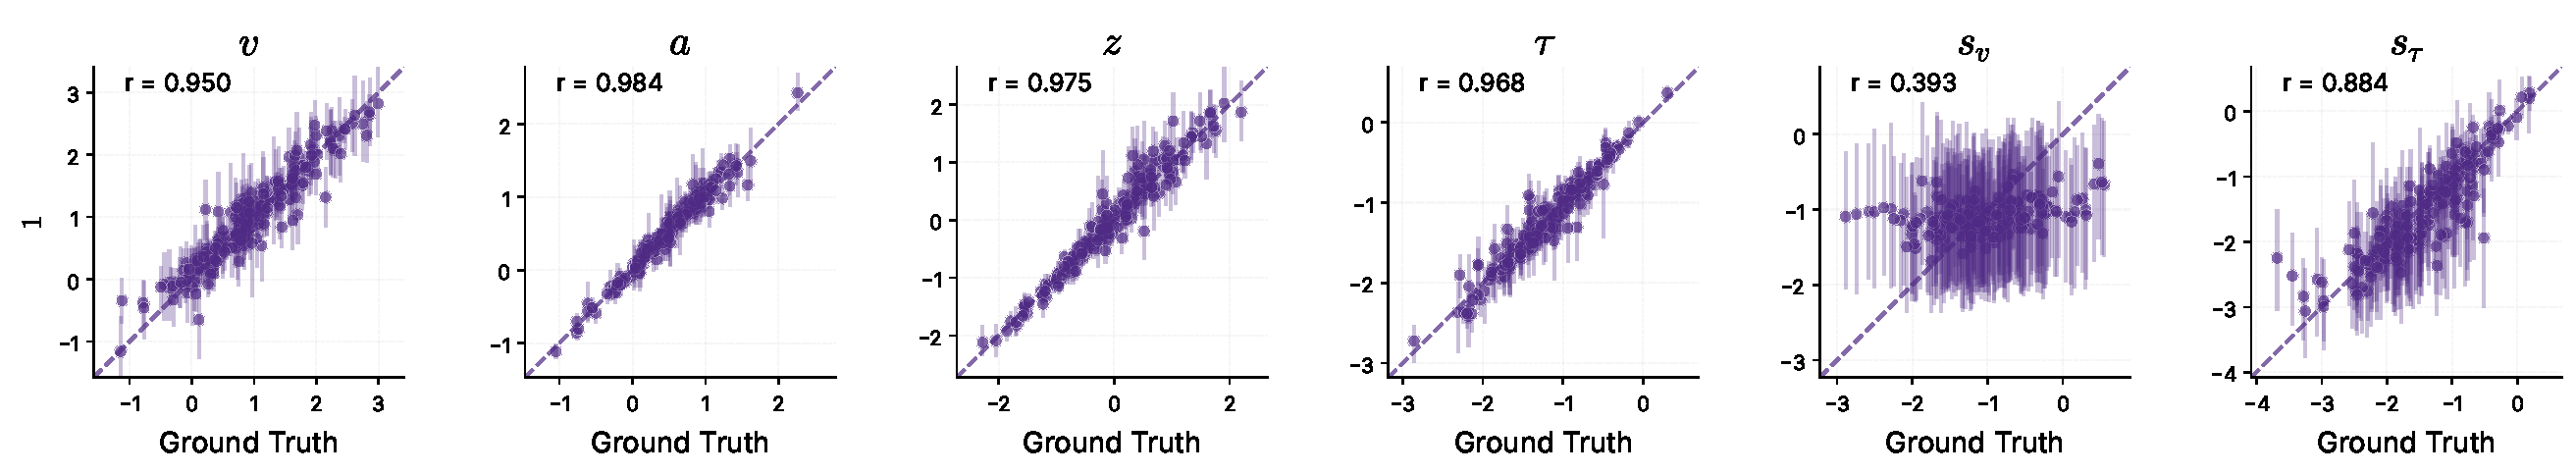
\includegraphics[width=\linewidth,height=0.84\textheight,keepaspectratio]{per_case/ddm/intercept_only/recovery.pdf}
  \caption[DDM, intercept-only: recovery]{\textbf{DDM, intercept-only design --- coefficient
    recovery.} Posterior mean (points) with 95\% credible intervals against the
    data-generating value, one panel per active cell of the coefficient matrix
    $\mathbf{B}$. Columns are intrinsic parameters, rows are design columns
    (intercept, main effects, interactions), labeled by regressor and category;
    the panel axes render this as \texttt{predictor|category}. Inactive cells are
    drawn as grey N/A tiles. Point color encodes the row kind: intercept (purple),
    main effect (blue), interaction (red).}
  \label{fig:e1-ddm-intercept_only-rec}
\end{figure}

\begin{figure}[htbp]
  \centering
  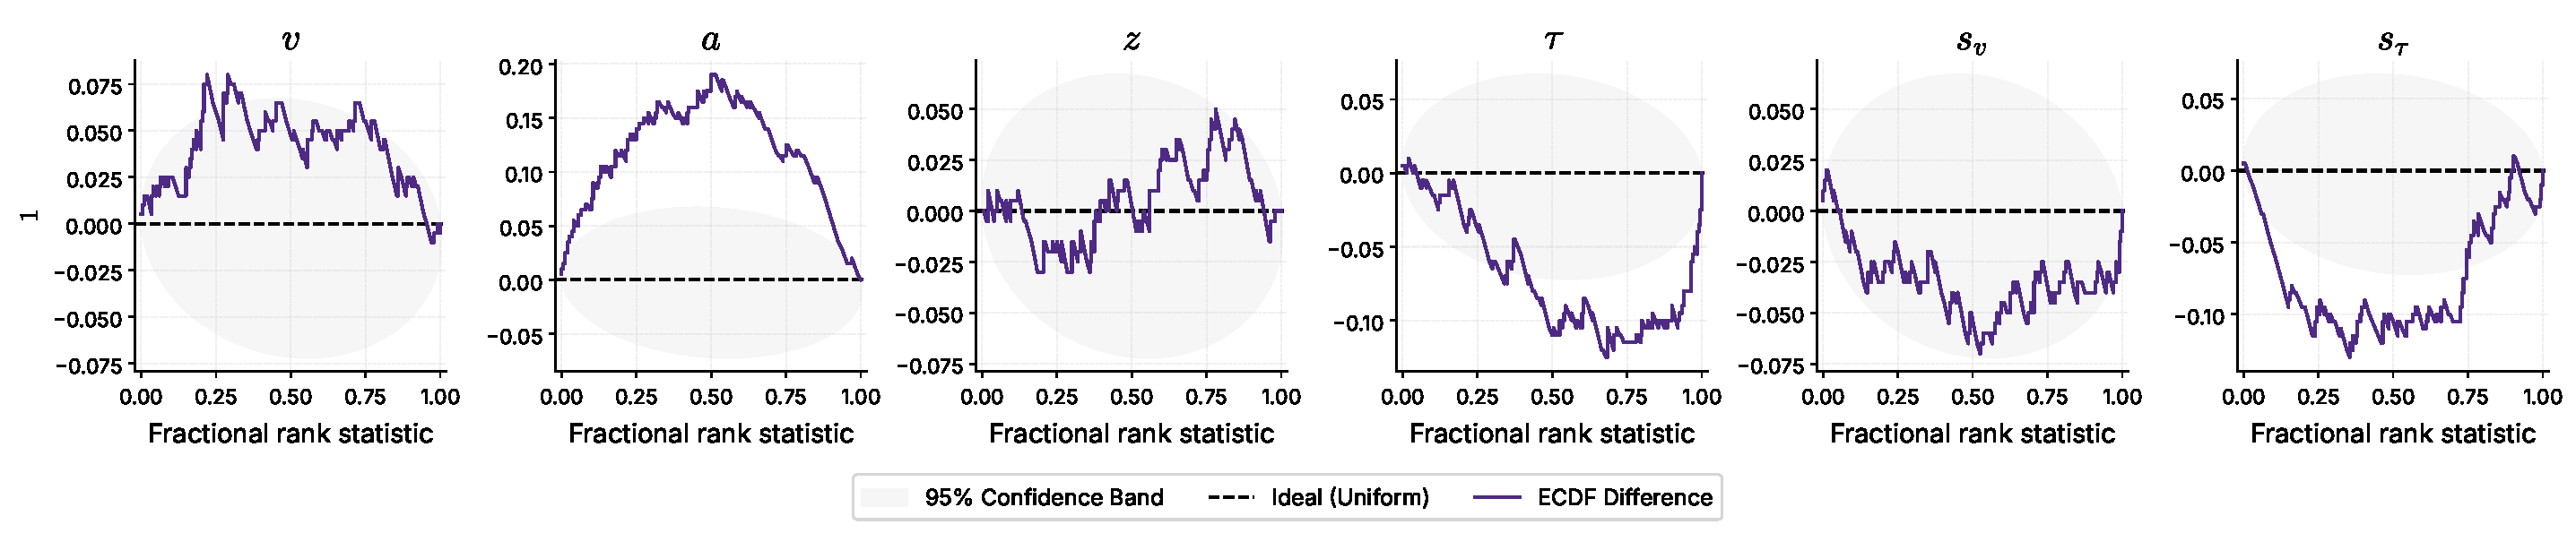
\includegraphics[width=\linewidth,height=0.84\textheight,keepaspectratio]{per_case/ddm/intercept_only/ecdf.pdf}
  \caption[DDM, intercept-only: ECDF calibration]{\textbf{DDM, intercept-only design --- ECDF
    calibration.} Rank-ECDF difference (empirical minus uniform) with simultaneous
    95\% confidence bands, on the same cell layout as the corresponding recovery
    figure (Figure~\ref{fig:e1-ddm-intercept_only-rec}). A calibrated posterior stays
    inside the band; excursions above/below indicate bias, and a systematically
    shallow/steep curve indicates over-/under-dispersion.}
  \label{fig:e1-ddm-intercept_only-ecdf}
\end{figure}

\begin{figure}[htbp]
  \centering
  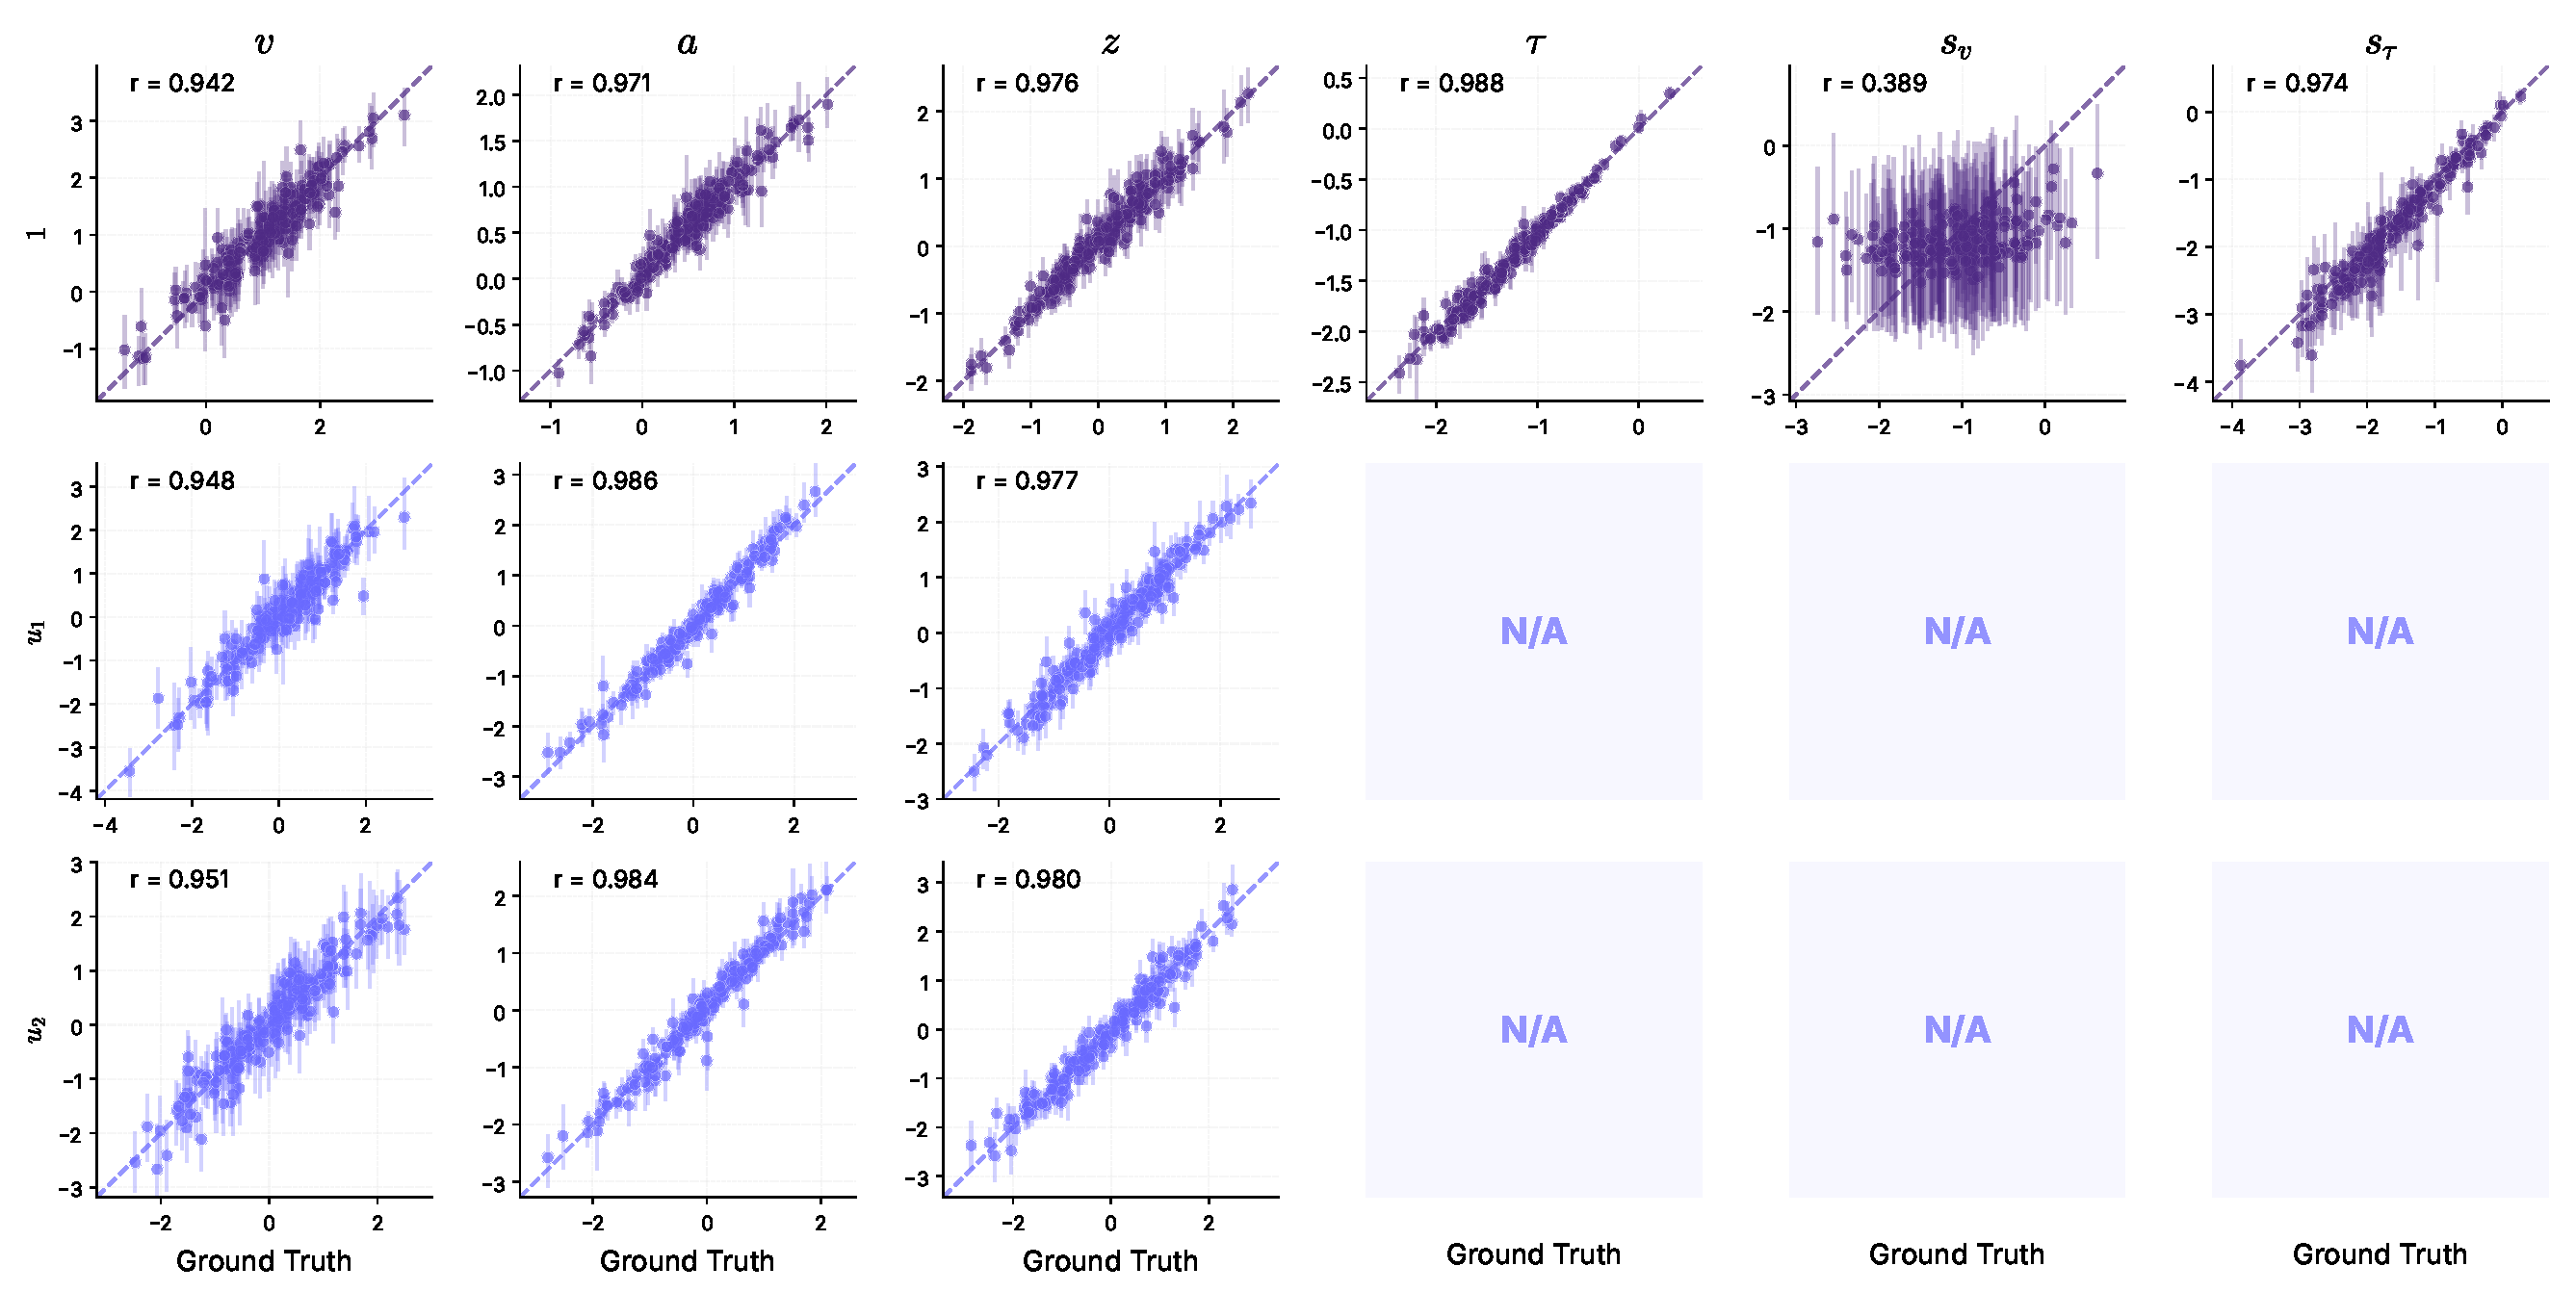
\includegraphics[width=\linewidth,height=0.84\textheight,keepaspectratio]{per_case/ddm/regressed/recovery.pdf}
  \caption[DDM, regressed: recovery]{\textbf{DDM, regressed design --- coefficient
    recovery.} Posterior mean (points) with 95\% credible intervals against the
    data-generating value, one panel per active cell of the coefficient matrix
    $\mathbf{B}$. Columns are intrinsic parameters, rows are design columns
    (intercept, main effects, interactions), labeled by regressor and category;
    the panel axes render this as \texttt{predictor|category}. Inactive cells are
    drawn as grey N/A tiles. Point color encodes the row kind: intercept (purple),
    main effect (blue), interaction (red).}
  \label{fig:e1-ddm-regressed-rec}
\end{figure}

\begin{figure}[htbp]
  \centering
  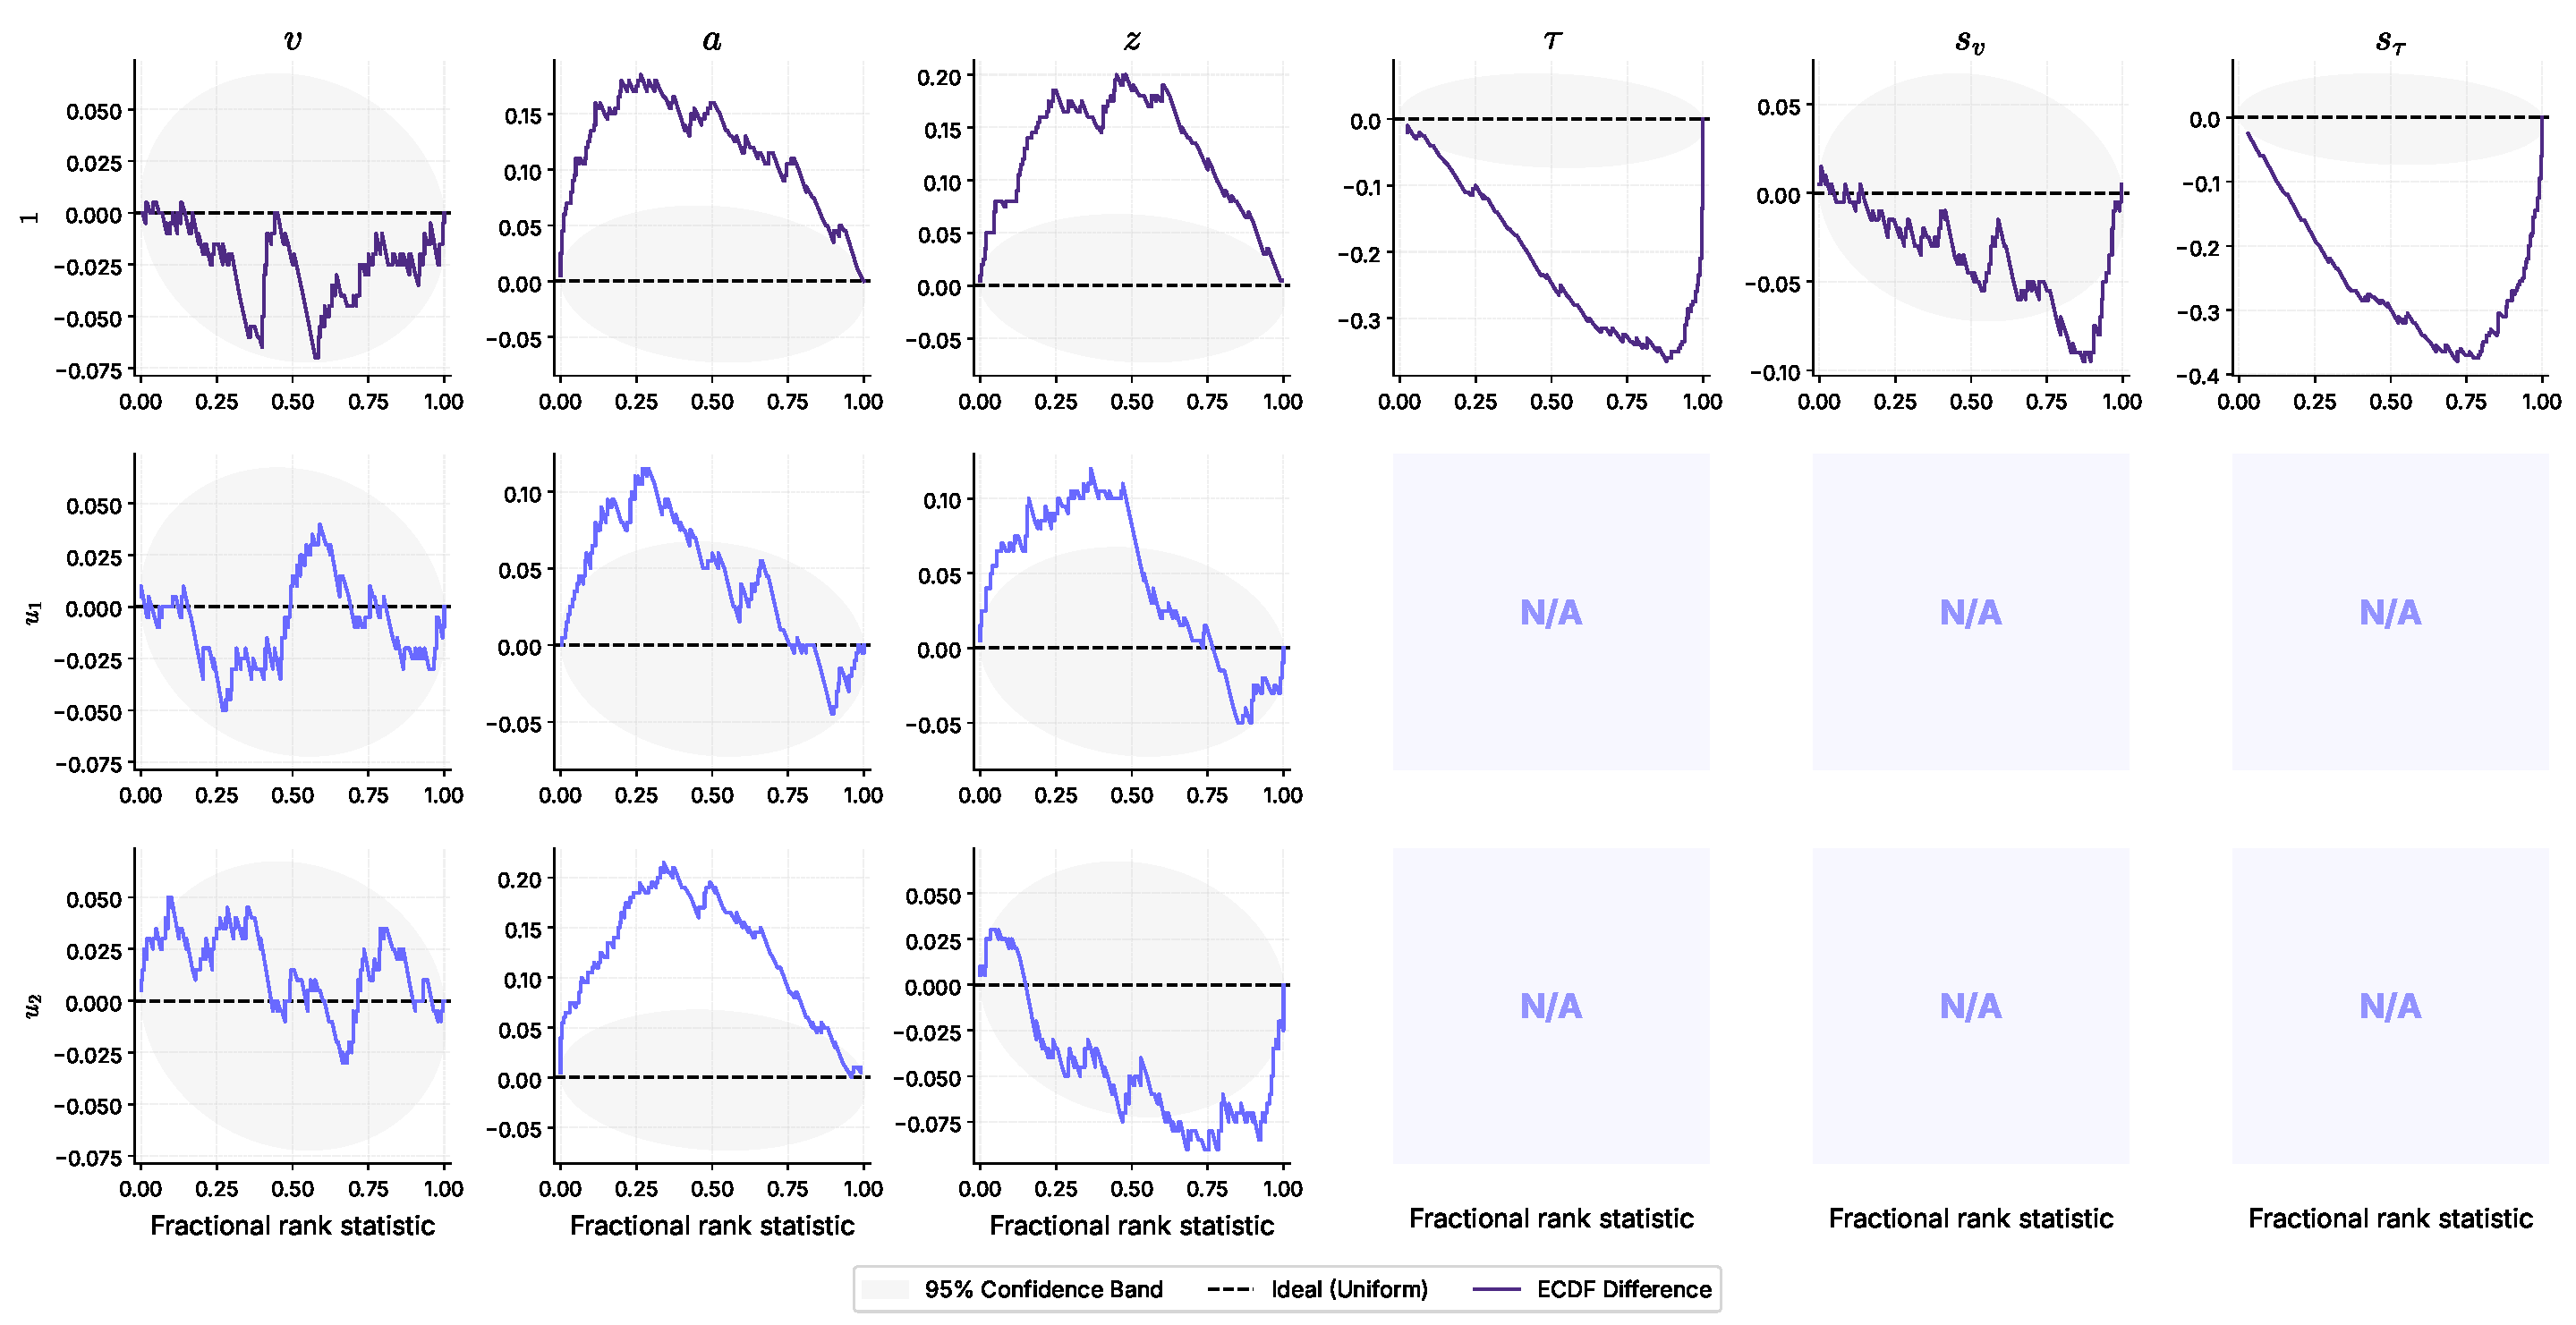
\includegraphics[width=\linewidth,height=0.84\textheight,keepaspectratio]{per_case/ddm/regressed/ecdf.pdf}
  \caption[DDM, regressed: ECDF calibration]{\textbf{DDM, regressed design --- ECDF
    calibration.} Rank-ECDF difference (empirical minus uniform) with simultaneous
    95\% confidence bands, on the same cell layout as the corresponding recovery
    figure (Figure~\ref{fig:e1-ddm-regressed-rec}). A calibrated posterior stays
    inside the band; excursions above/below indicate bias, and a systematically
    shallow/steep curve indicates over-/under-dispersion.}
  \label{fig:e1-ddm-regressed-ecdf}
\end{figure}

\begin{figure}[htbp]
  \centering
  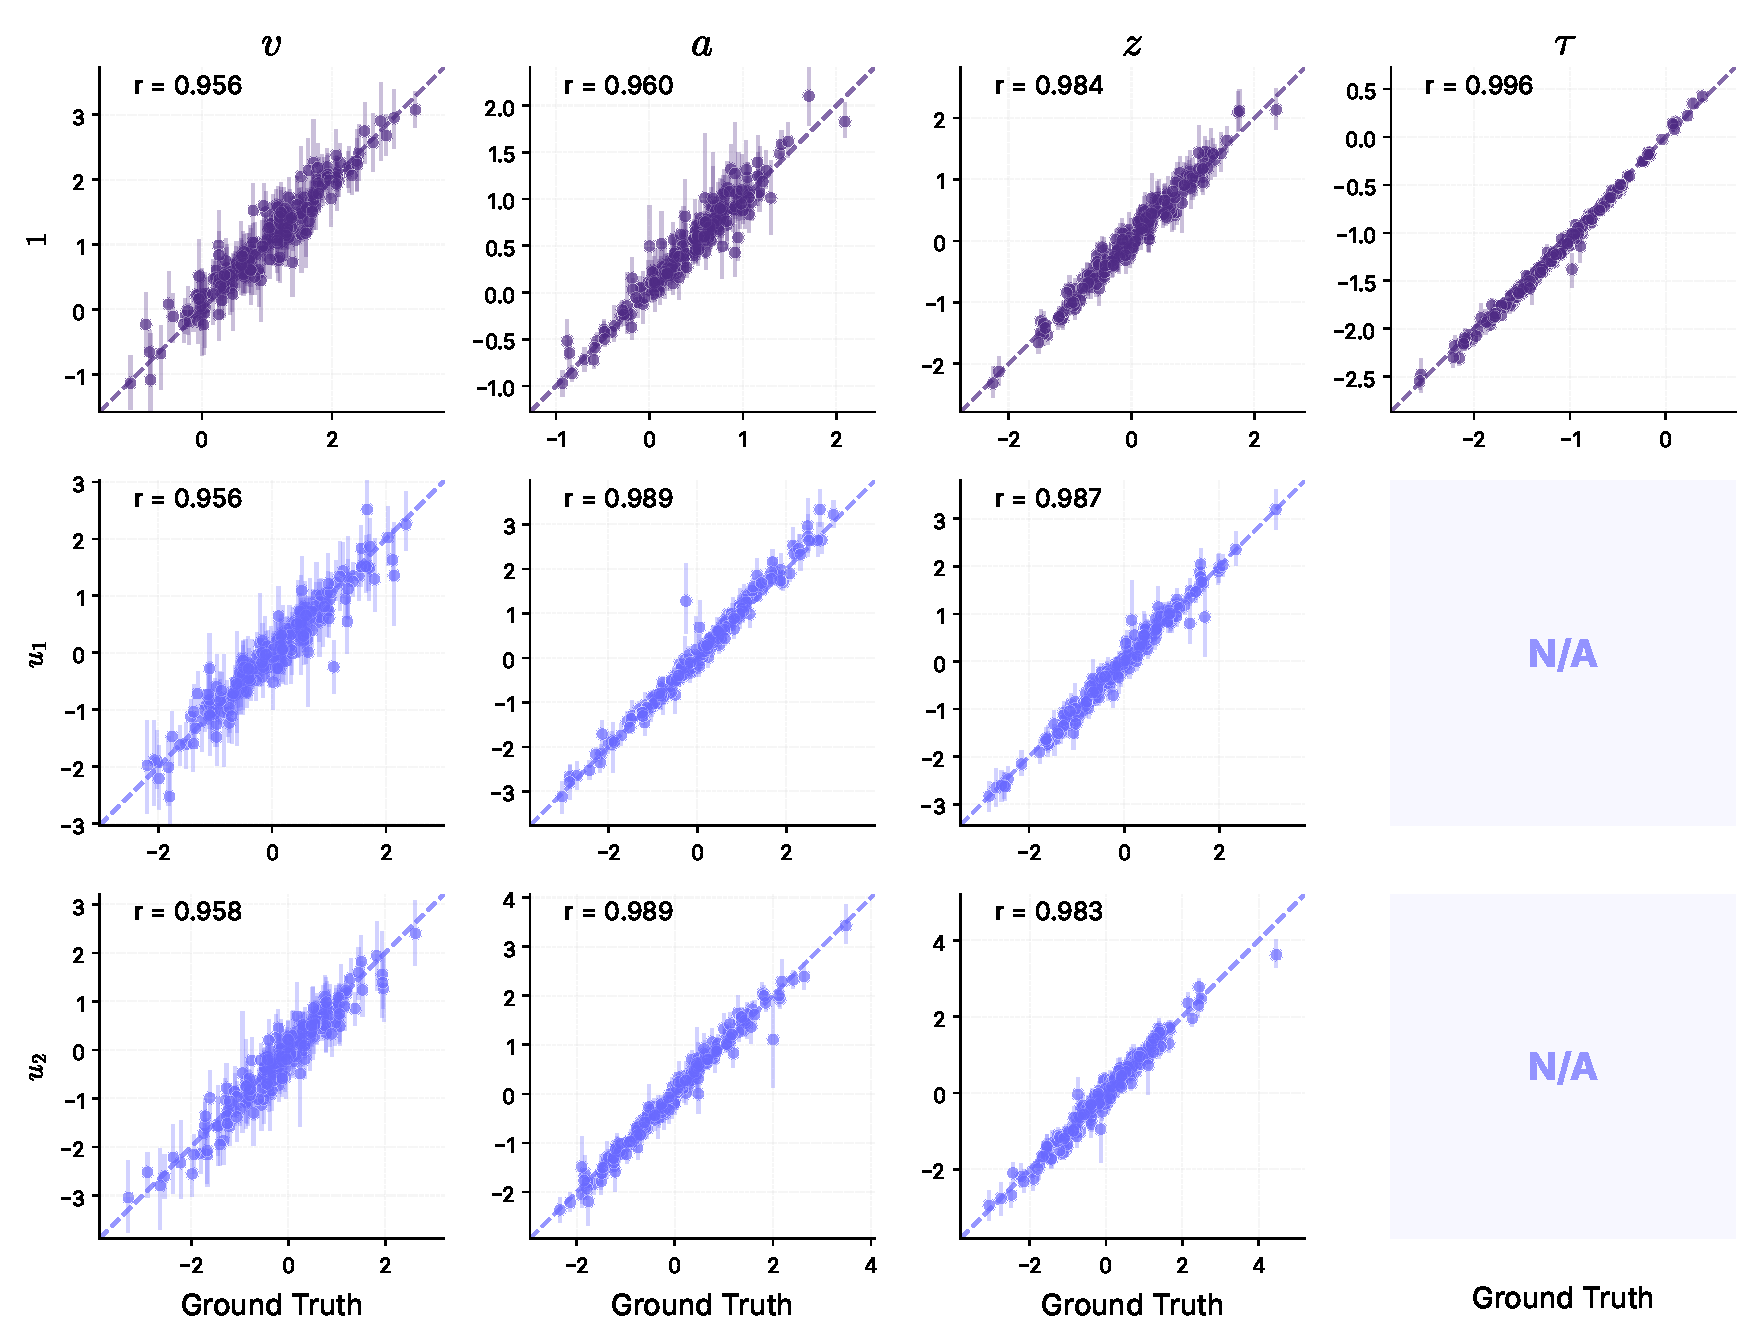
\includegraphics[width=\linewidth,height=0.84\textheight,keepaspectratio]{per_case/ddm/fixed_regressed/recovery.pdf}
  \caption[DDM, fixed-regressed: recovery]{\textbf{DDM, fixed-regressed design --- coefficient
    recovery.} Posterior mean (points) with 95\% credible intervals against the
    data-generating value, one panel per active cell of the coefficient matrix
    $\mathbf{B}$. Columns are intrinsic parameters, rows are design columns
    (intercept, main effects, interactions), labeled by regressor and category;
    the panel axes render this as \texttt{predictor|category}. Inactive cells are
    drawn as grey N/A tiles. Point color encodes the row kind: intercept (purple),
    main effect (blue), interaction (red).}
  \label{fig:e1-ddm-fixed_regressed-rec}
\end{figure}

\begin{figure}[htbp]
  \centering
  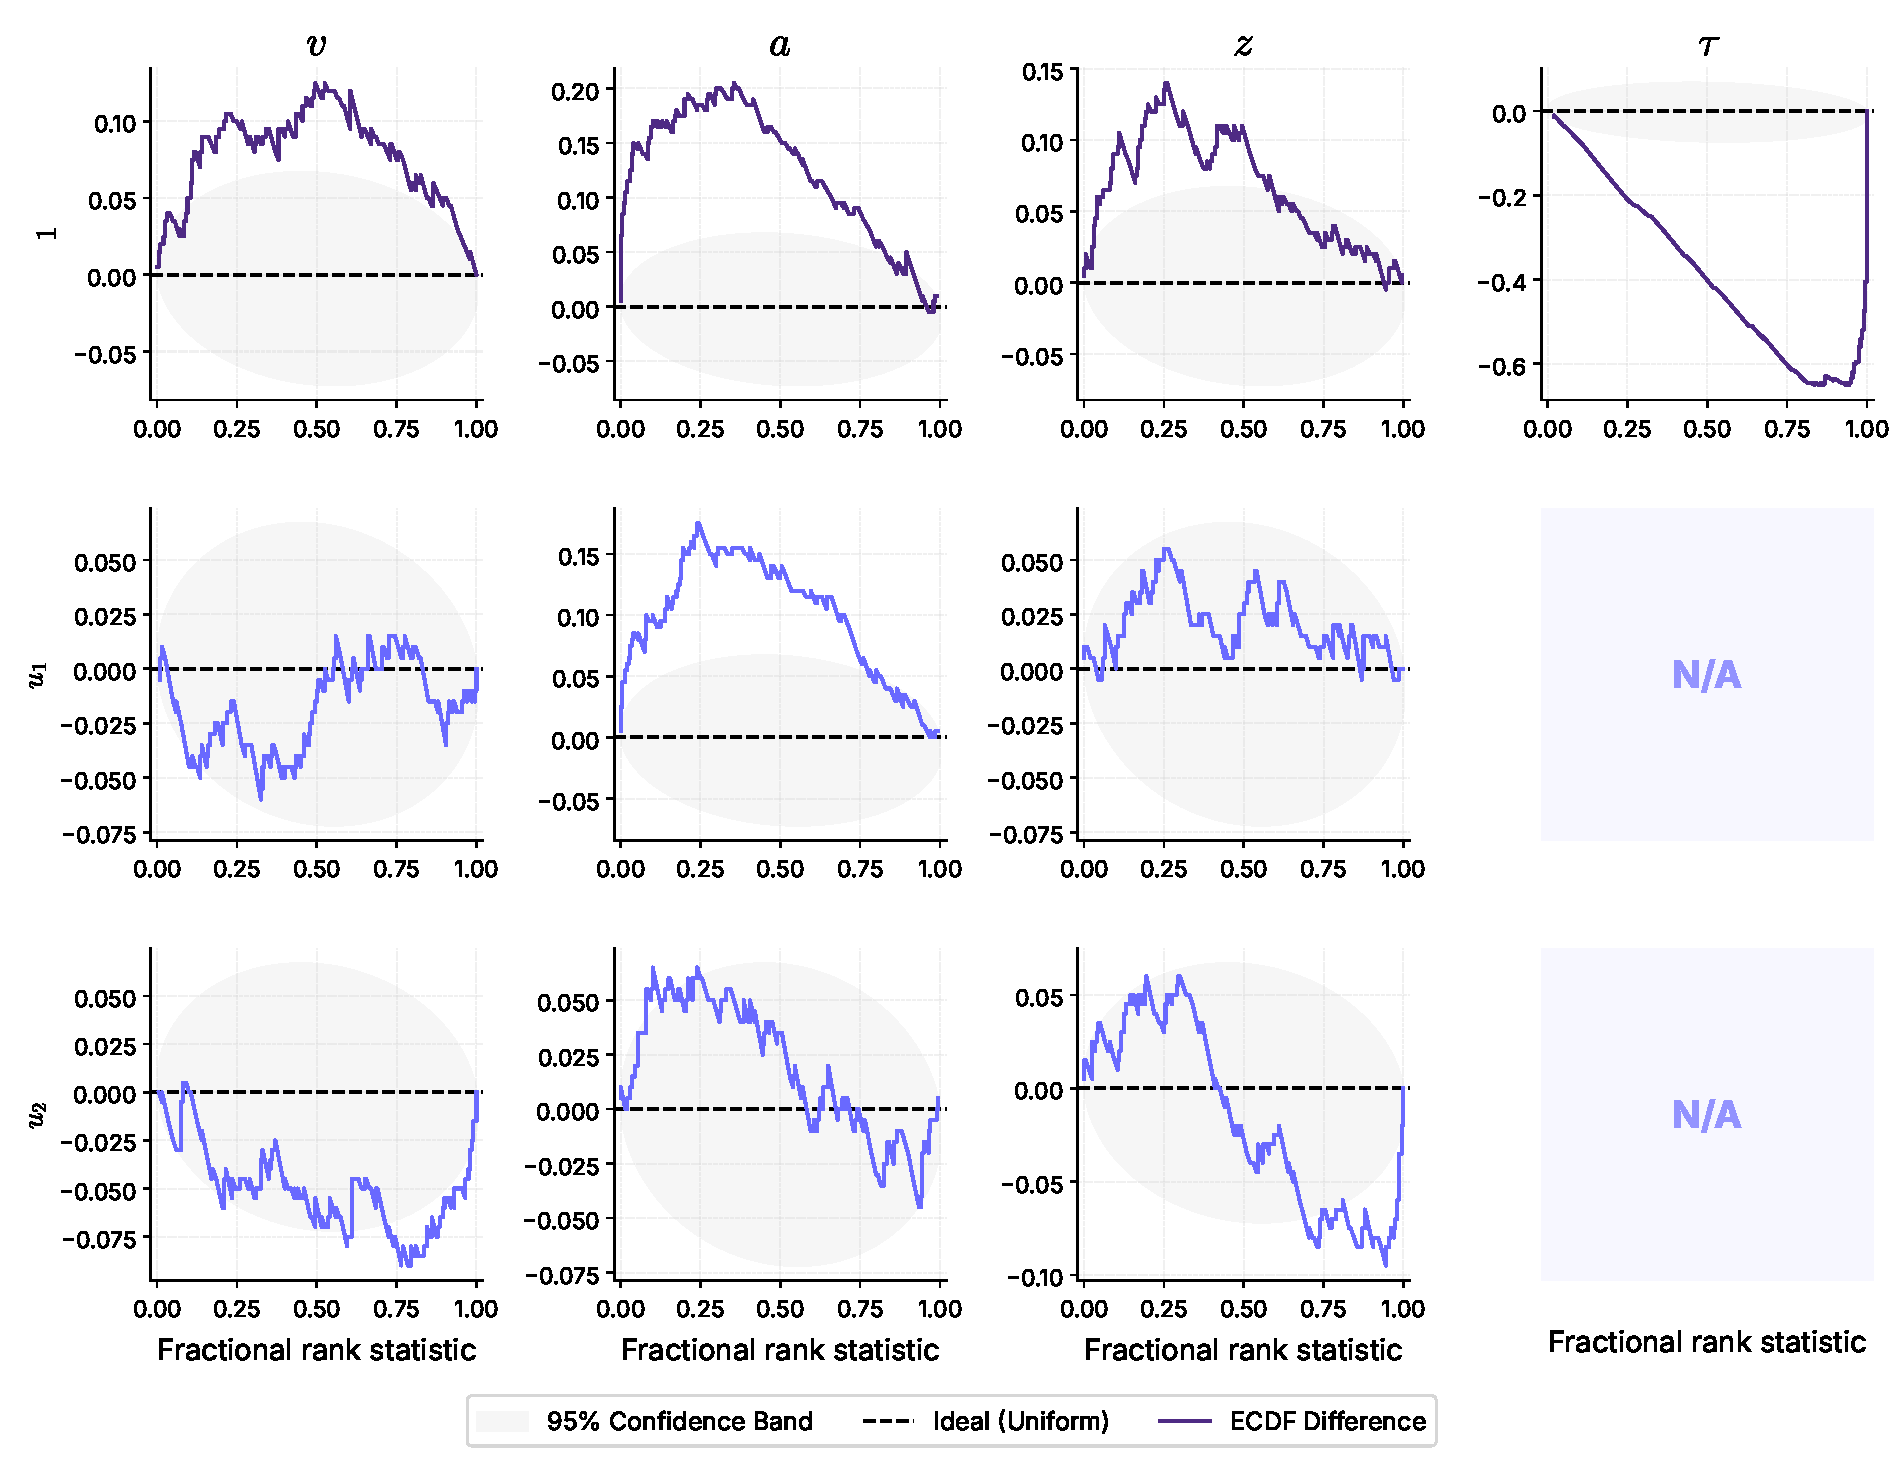
\includegraphics[width=\linewidth,height=0.84\textheight,keepaspectratio]{per_case/ddm/fixed_regressed/ecdf.pdf}
  \caption[DDM, fixed-regressed: ECDF calibration]{\textbf{DDM, fixed-regressed design --- ECDF
    calibration.} Rank-ECDF difference (empirical minus uniform) with simultaneous
    95\% confidence bands, on the same cell layout as the corresponding recovery
    figure (Figure~\ref{fig:e1-ddm-fixed_regressed-rec}). A calibrated posterior stays
    inside the band; excursions above/below indicate bias, and a systematically
    shallow/steep curve indicates over-/under-dispersion.}
  \label{fig:e1-ddm-fixed_regressed-ecdf}
\end{figure}

\begin{figure}[htbp]
  \centering
  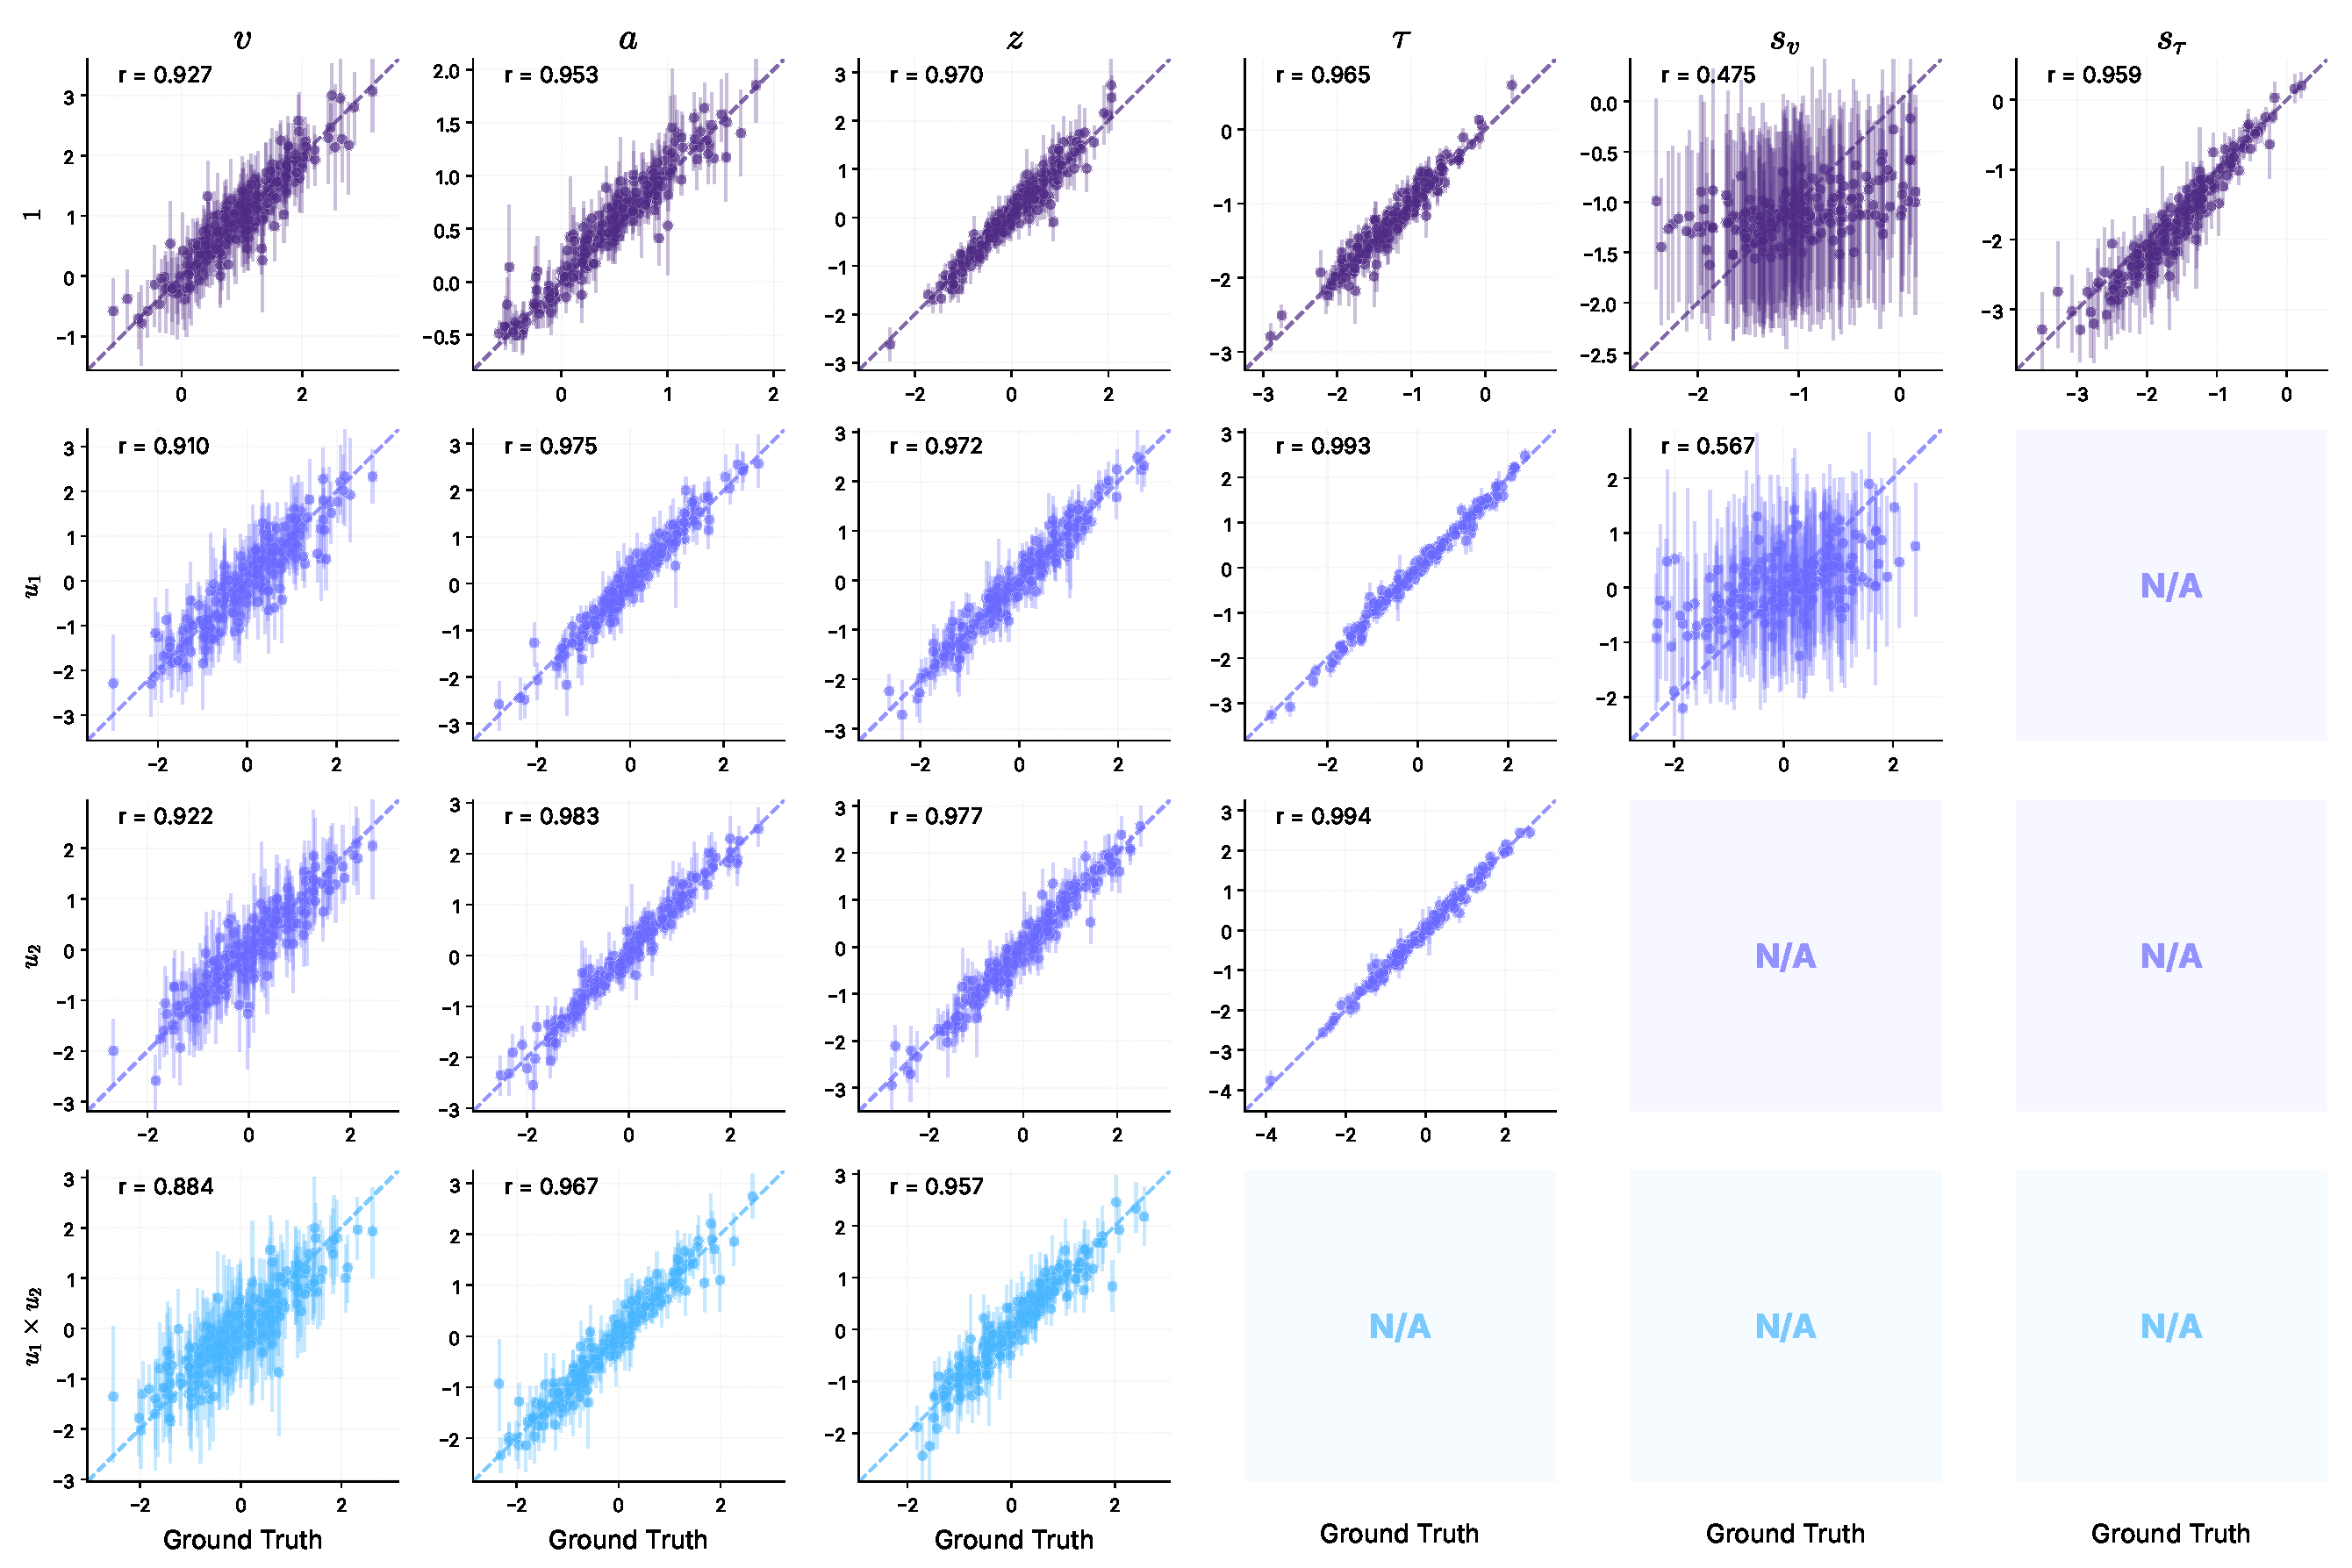
\includegraphics[width=\linewidth,height=0.84\textheight,keepaspectratio]{per_case/ddm/interaction/recovery.pdf}
  \caption[DDM, interaction: recovery]{\textbf{DDM, interaction design --- coefficient
    recovery.} Posterior mean (points) with 95\% credible intervals against the
    data-generating value, one panel per active cell of the coefficient matrix
    $\mathbf{B}$. Columns are intrinsic parameters, rows are design columns
    (intercept, main effects, interactions), labeled by regressor and category;
    the panel axes render this as \texttt{predictor|category}. Inactive cells are
    drawn as grey N/A tiles. Point color encodes the row kind: intercept (purple),
    main effect (blue), interaction (red).}
  \label{fig:e1-ddm-interaction-rec}
\end{figure}

\begin{figure}[htbp]
  \centering
  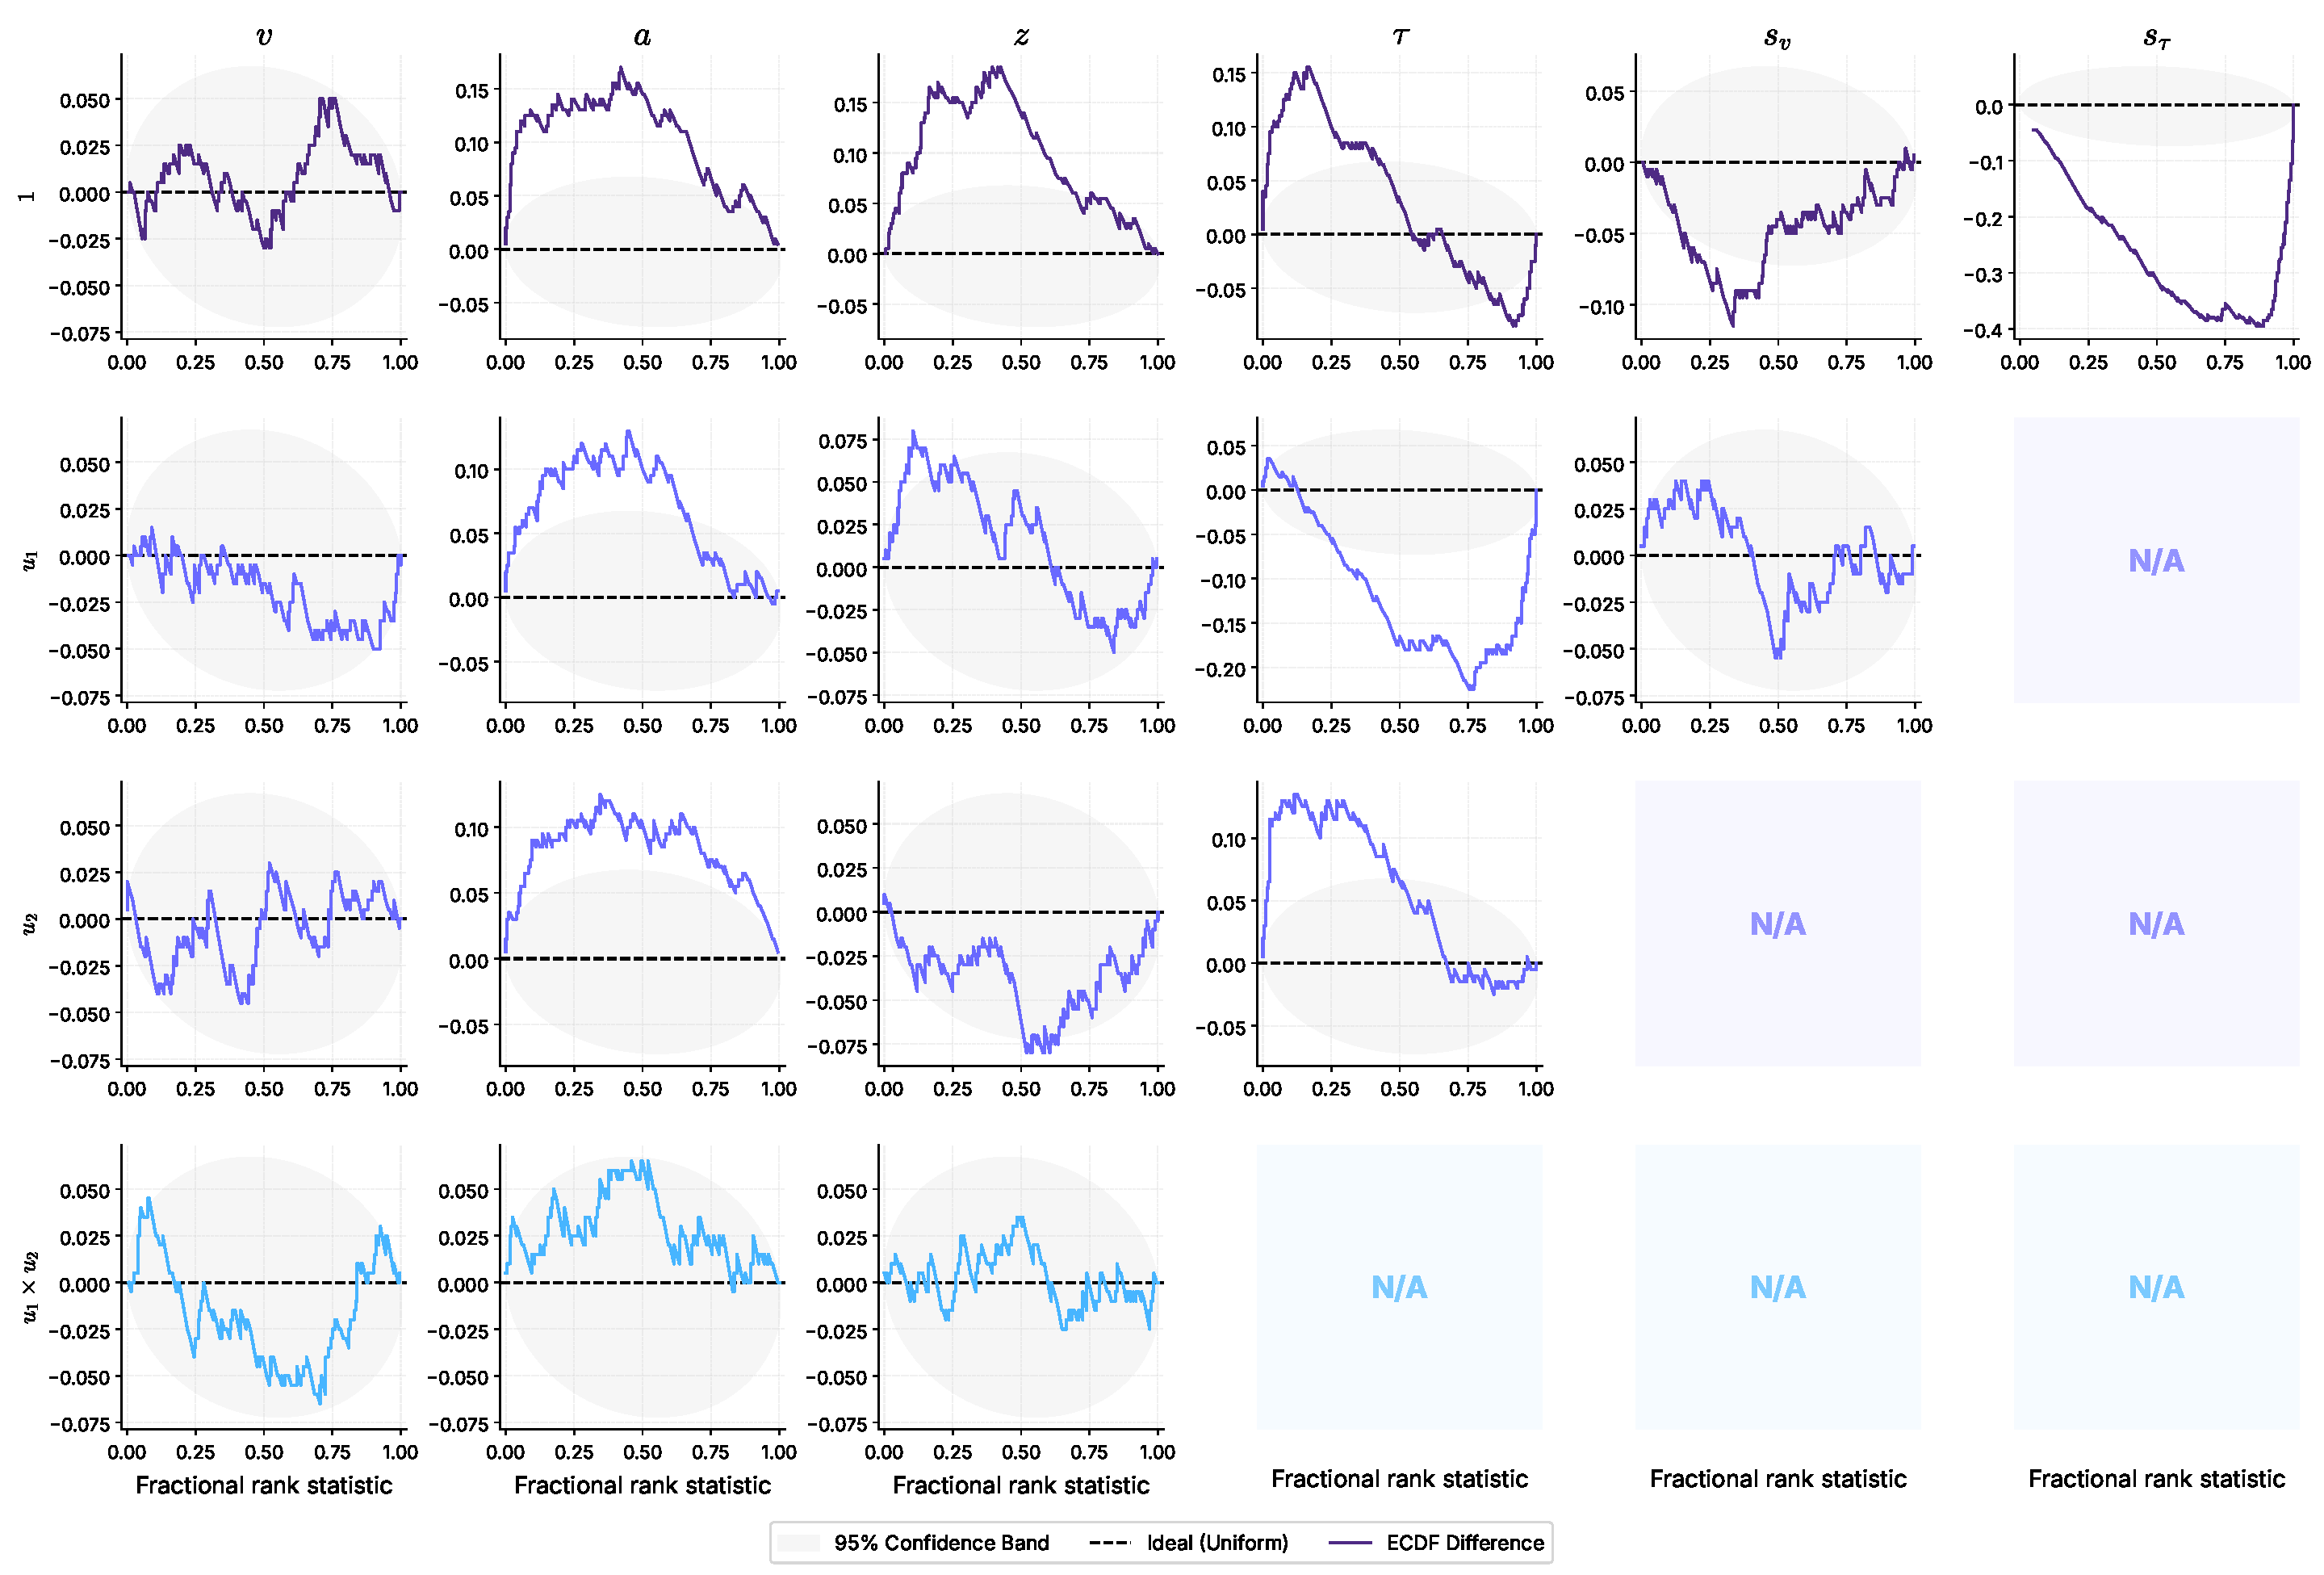
\includegraphics[width=\linewidth,height=0.84\textheight,keepaspectratio]{per_case/ddm/interaction/ecdf.pdf}
  \caption[DDM, interaction: ECDF calibration]{\textbf{DDM, interaction design --- ECDF
    calibration.} Rank-ECDF difference (empirical minus uniform) with simultaneous
    95\% confidence bands, on the same cell layout as the corresponding recovery
    figure (Figure~\ref{fig:e1-ddm-interaction-rec}). A calibrated posterior stays
    inside the band; excursions above/below indicate bias, and a systematically
    shallow/steep curve indicates over-/under-dispersion.}
  \label{fig:e1-ddm-interaction-ecdf}
\end{figure}

\begin{figure}[htbp]
  \centering
  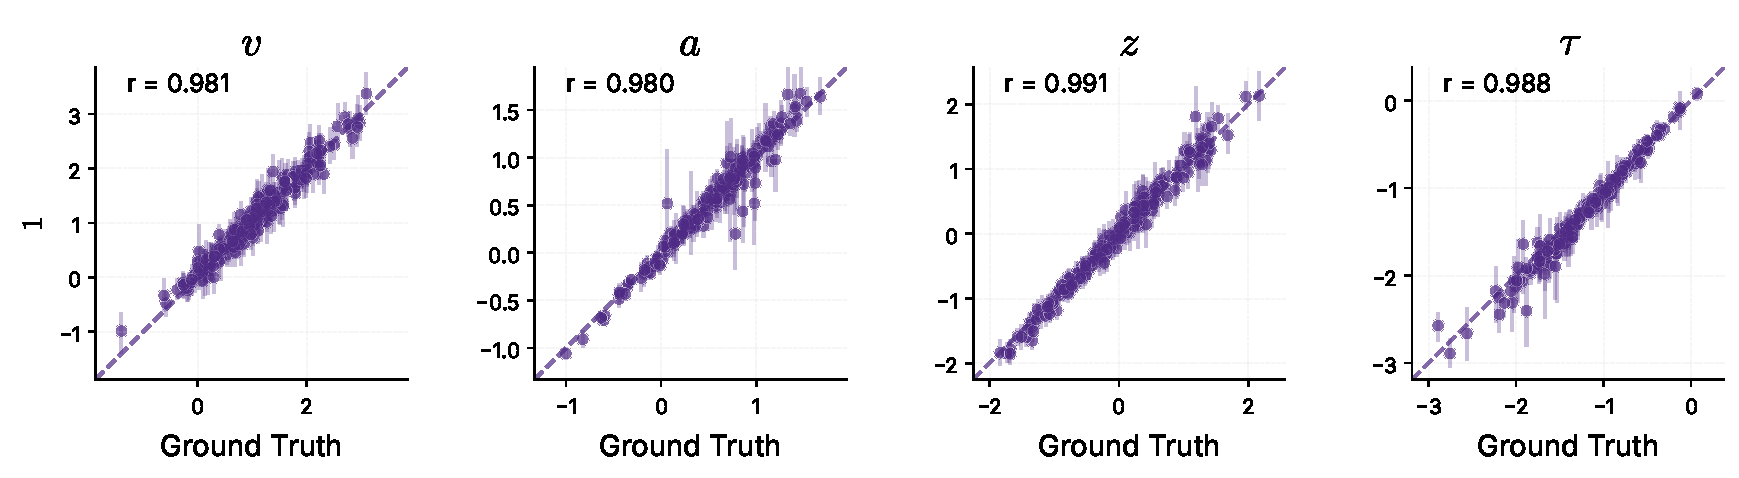
\includegraphics[width=\linewidth,height=0.84\textheight,keepaspectratio]{per_case/ddm/fixed/recovery.pdf}
  \caption[DDM, fixed: recovery]{\textbf{DDM, fixed design --- coefficient
    recovery.} Posterior mean (points) with 95\% credible intervals against the
    data-generating value, one panel per active cell of the coefficient matrix
    $\mathbf{B}$. Columns are intrinsic parameters, rows are design columns
    (intercept, main effects, interactions), labeled by regressor and category;
    the panel axes render this as \texttt{predictor|category}. Inactive cells are
    drawn as grey N/A tiles. Point color encodes the row kind: intercept (purple),
    main effect (blue), interaction (red).}
  \label{fig:e1-ddm-fixed-rec}
\end{figure}

\begin{figure}[htbp]
  \centering
  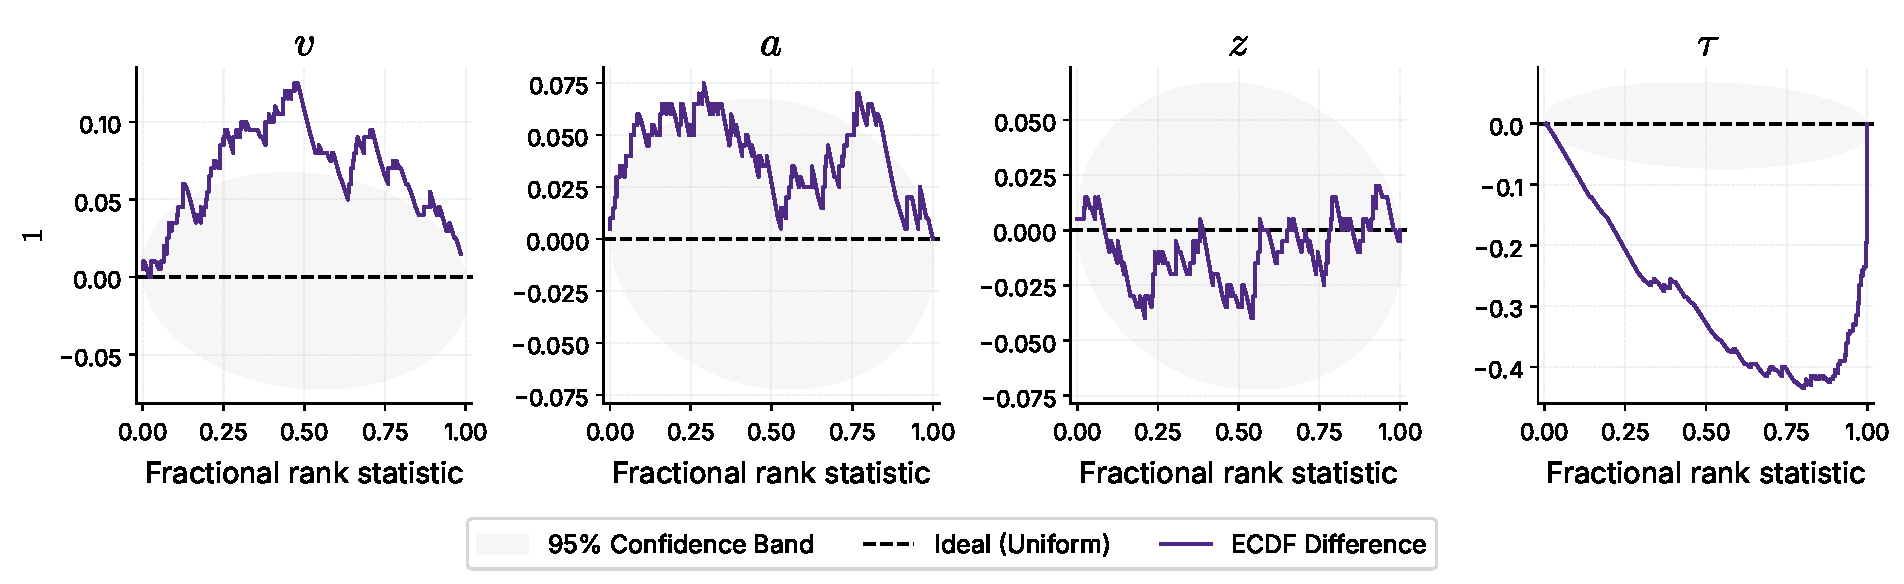
\includegraphics[width=\linewidth,height=0.84\textheight,keepaspectratio]{per_case/ddm/fixed/ecdf.pdf}
  \caption[DDM, fixed: ECDF calibration]{\textbf{DDM, fixed design --- ECDF
    calibration.} Rank-ECDF difference (empirical minus uniform) with simultaneous
    95\% confidence bands, on the same cell layout as the corresponding recovery
    figure (Figure~\ref{fig:e1-ddm-fixed-rec}). A calibrated posterior stays
    inside the band; excursions above/below indicate bias, and a systematically
    shallow/steep curve indicates over-/under-dispersion.}
  \label{fig:e1-ddm-fixed-ecdf}
\end{figure}

\begin{figure}[htbp]
  \centering
  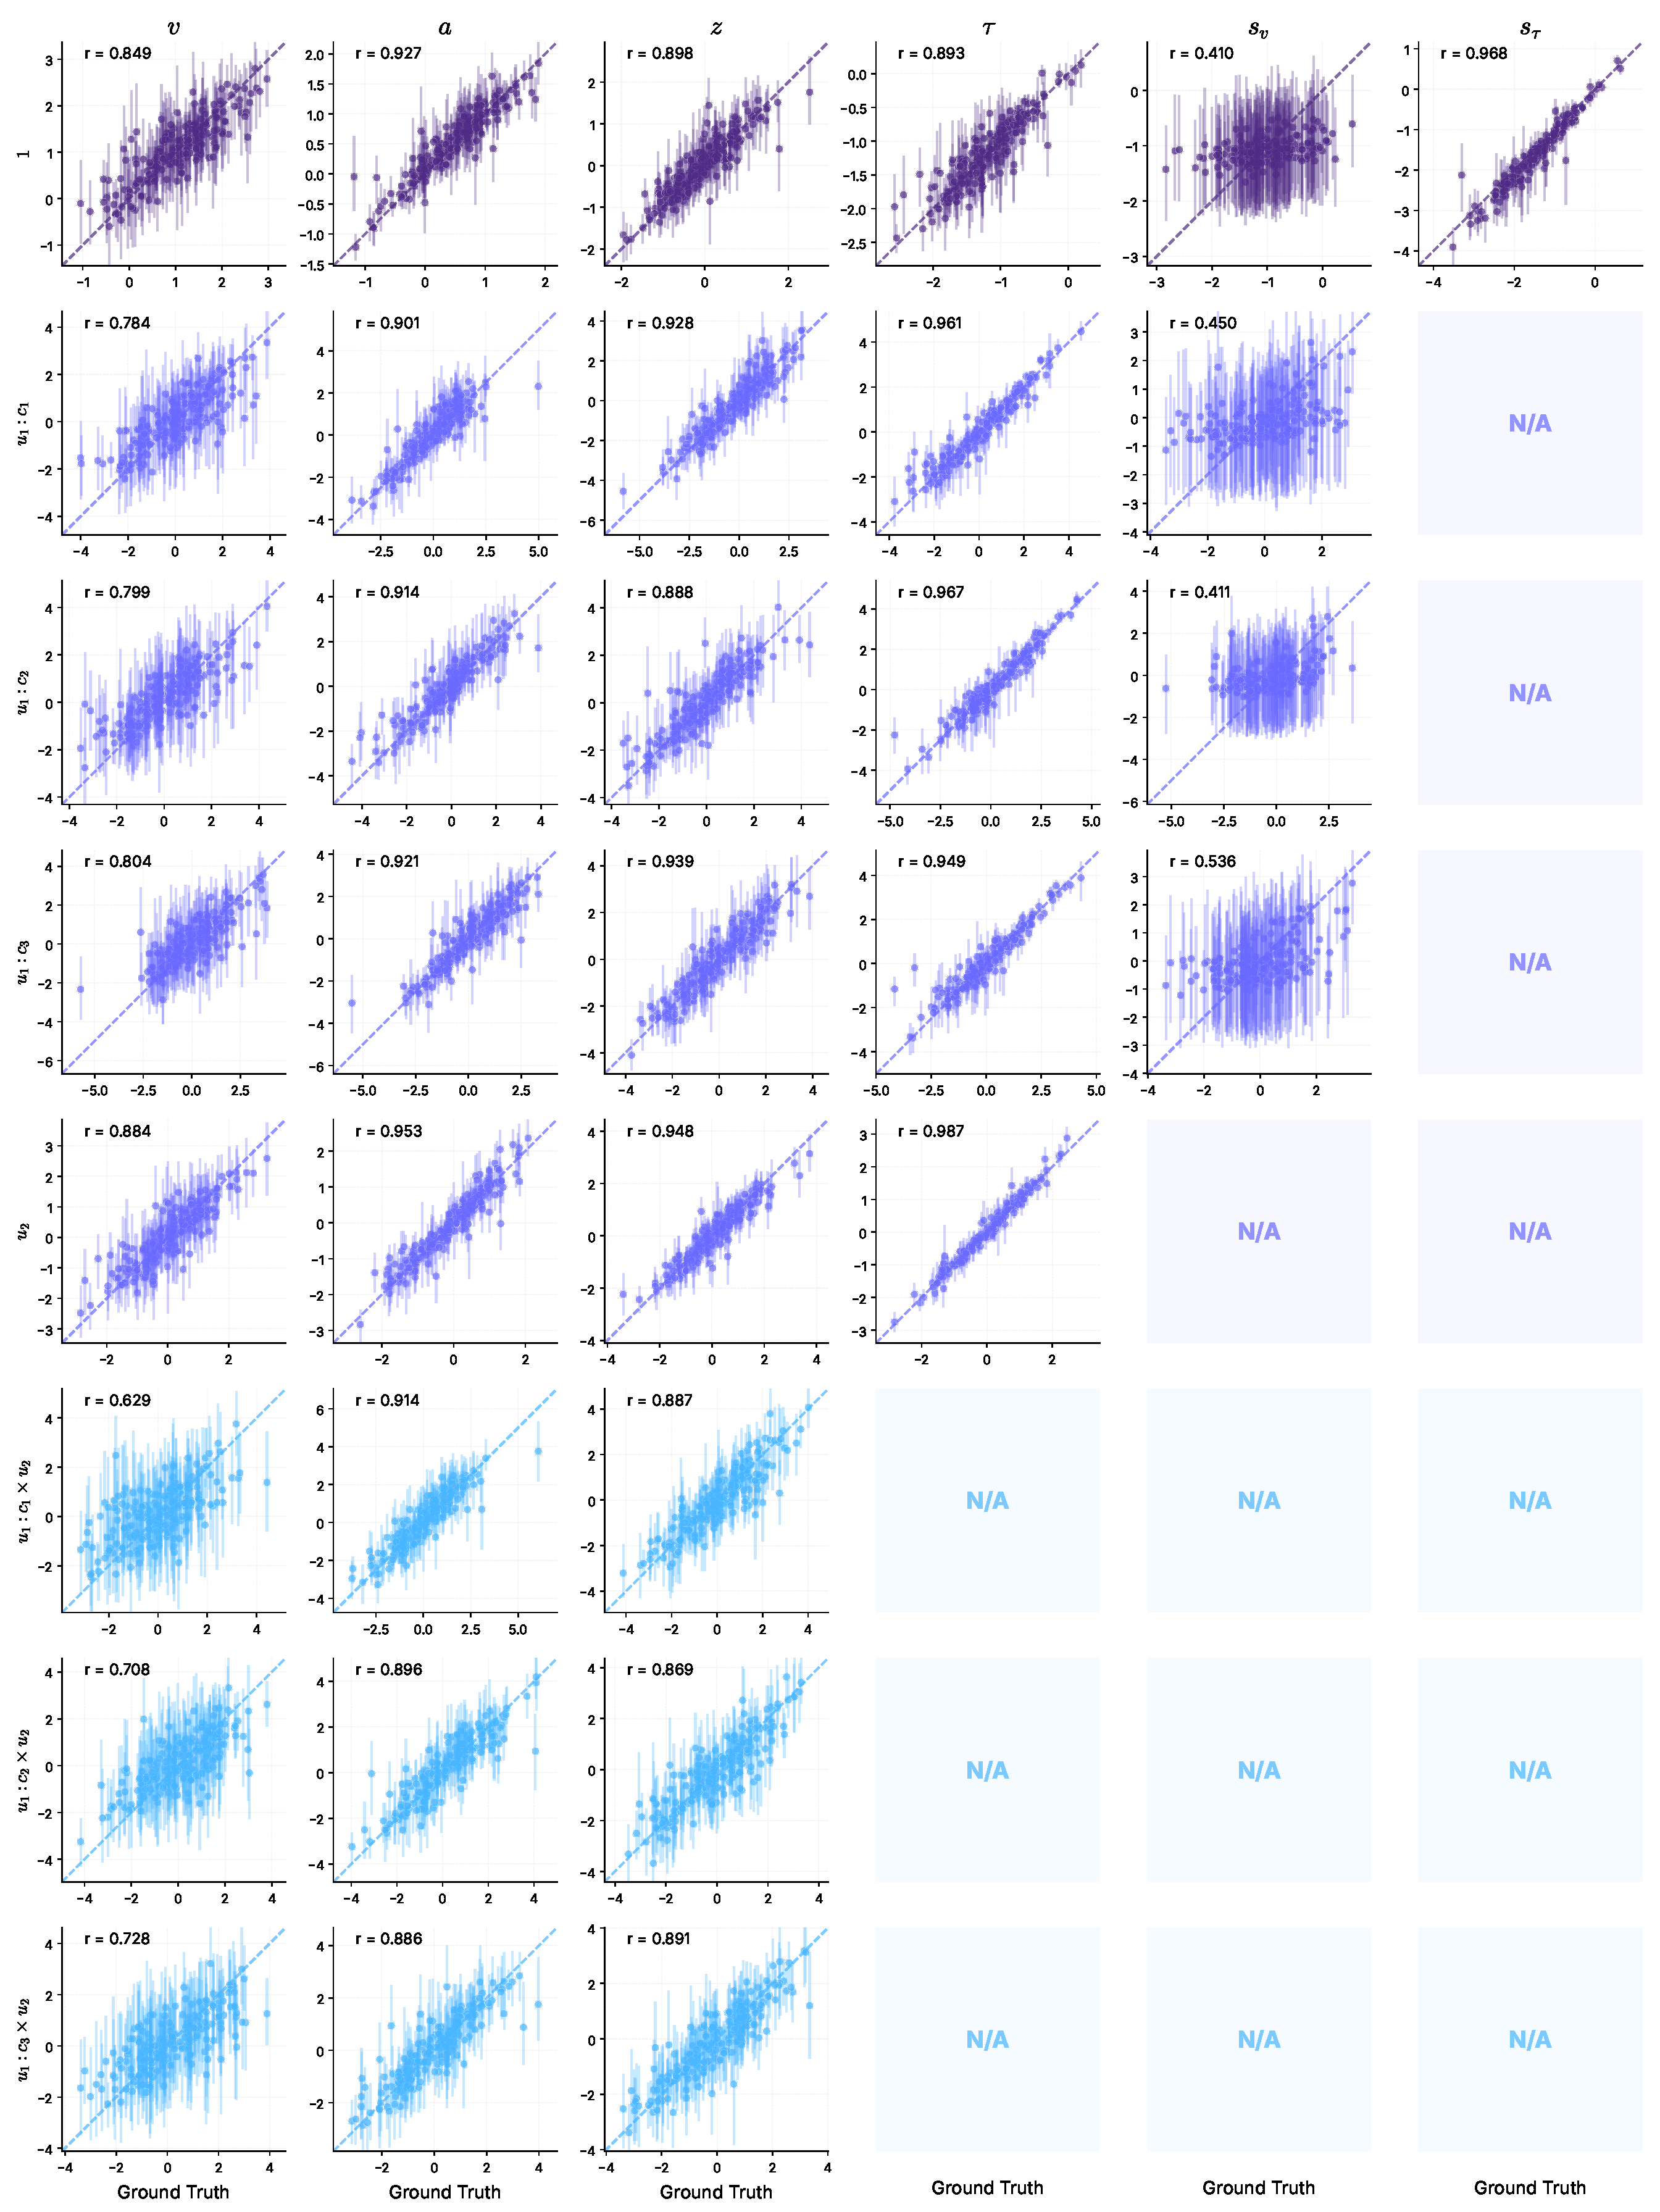
\includegraphics[width=\linewidth,height=0.84\textheight,keepaspectratio]{per_case/ddm/mixed_predictor/recovery.pdf}
  \caption[DDM, mixed-predictor: recovery]{\textbf{DDM, mixed-predictor design --- coefficient
    recovery.} Posterior mean (points) with 95\% credible intervals against the
    data-generating value, one panel per active cell of the coefficient matrix
    $\mathbf{B}$. Columns are intrinsic parameters, rows are design columns
    (intercept, main effects, interactions), labeled by regressor and category;
    the panel axes render this as \texttt{predictor|category}. Inactive cells are
    drawn as grey N/A tiles. Point color encodes the row kind: intercept (purple),
    main effect (blue), interaction (red).}
  \label{fig:e1-ddm-mixed_predictor-rec}
\end{figure}

\begin{figure}[htbp]
  \centering
  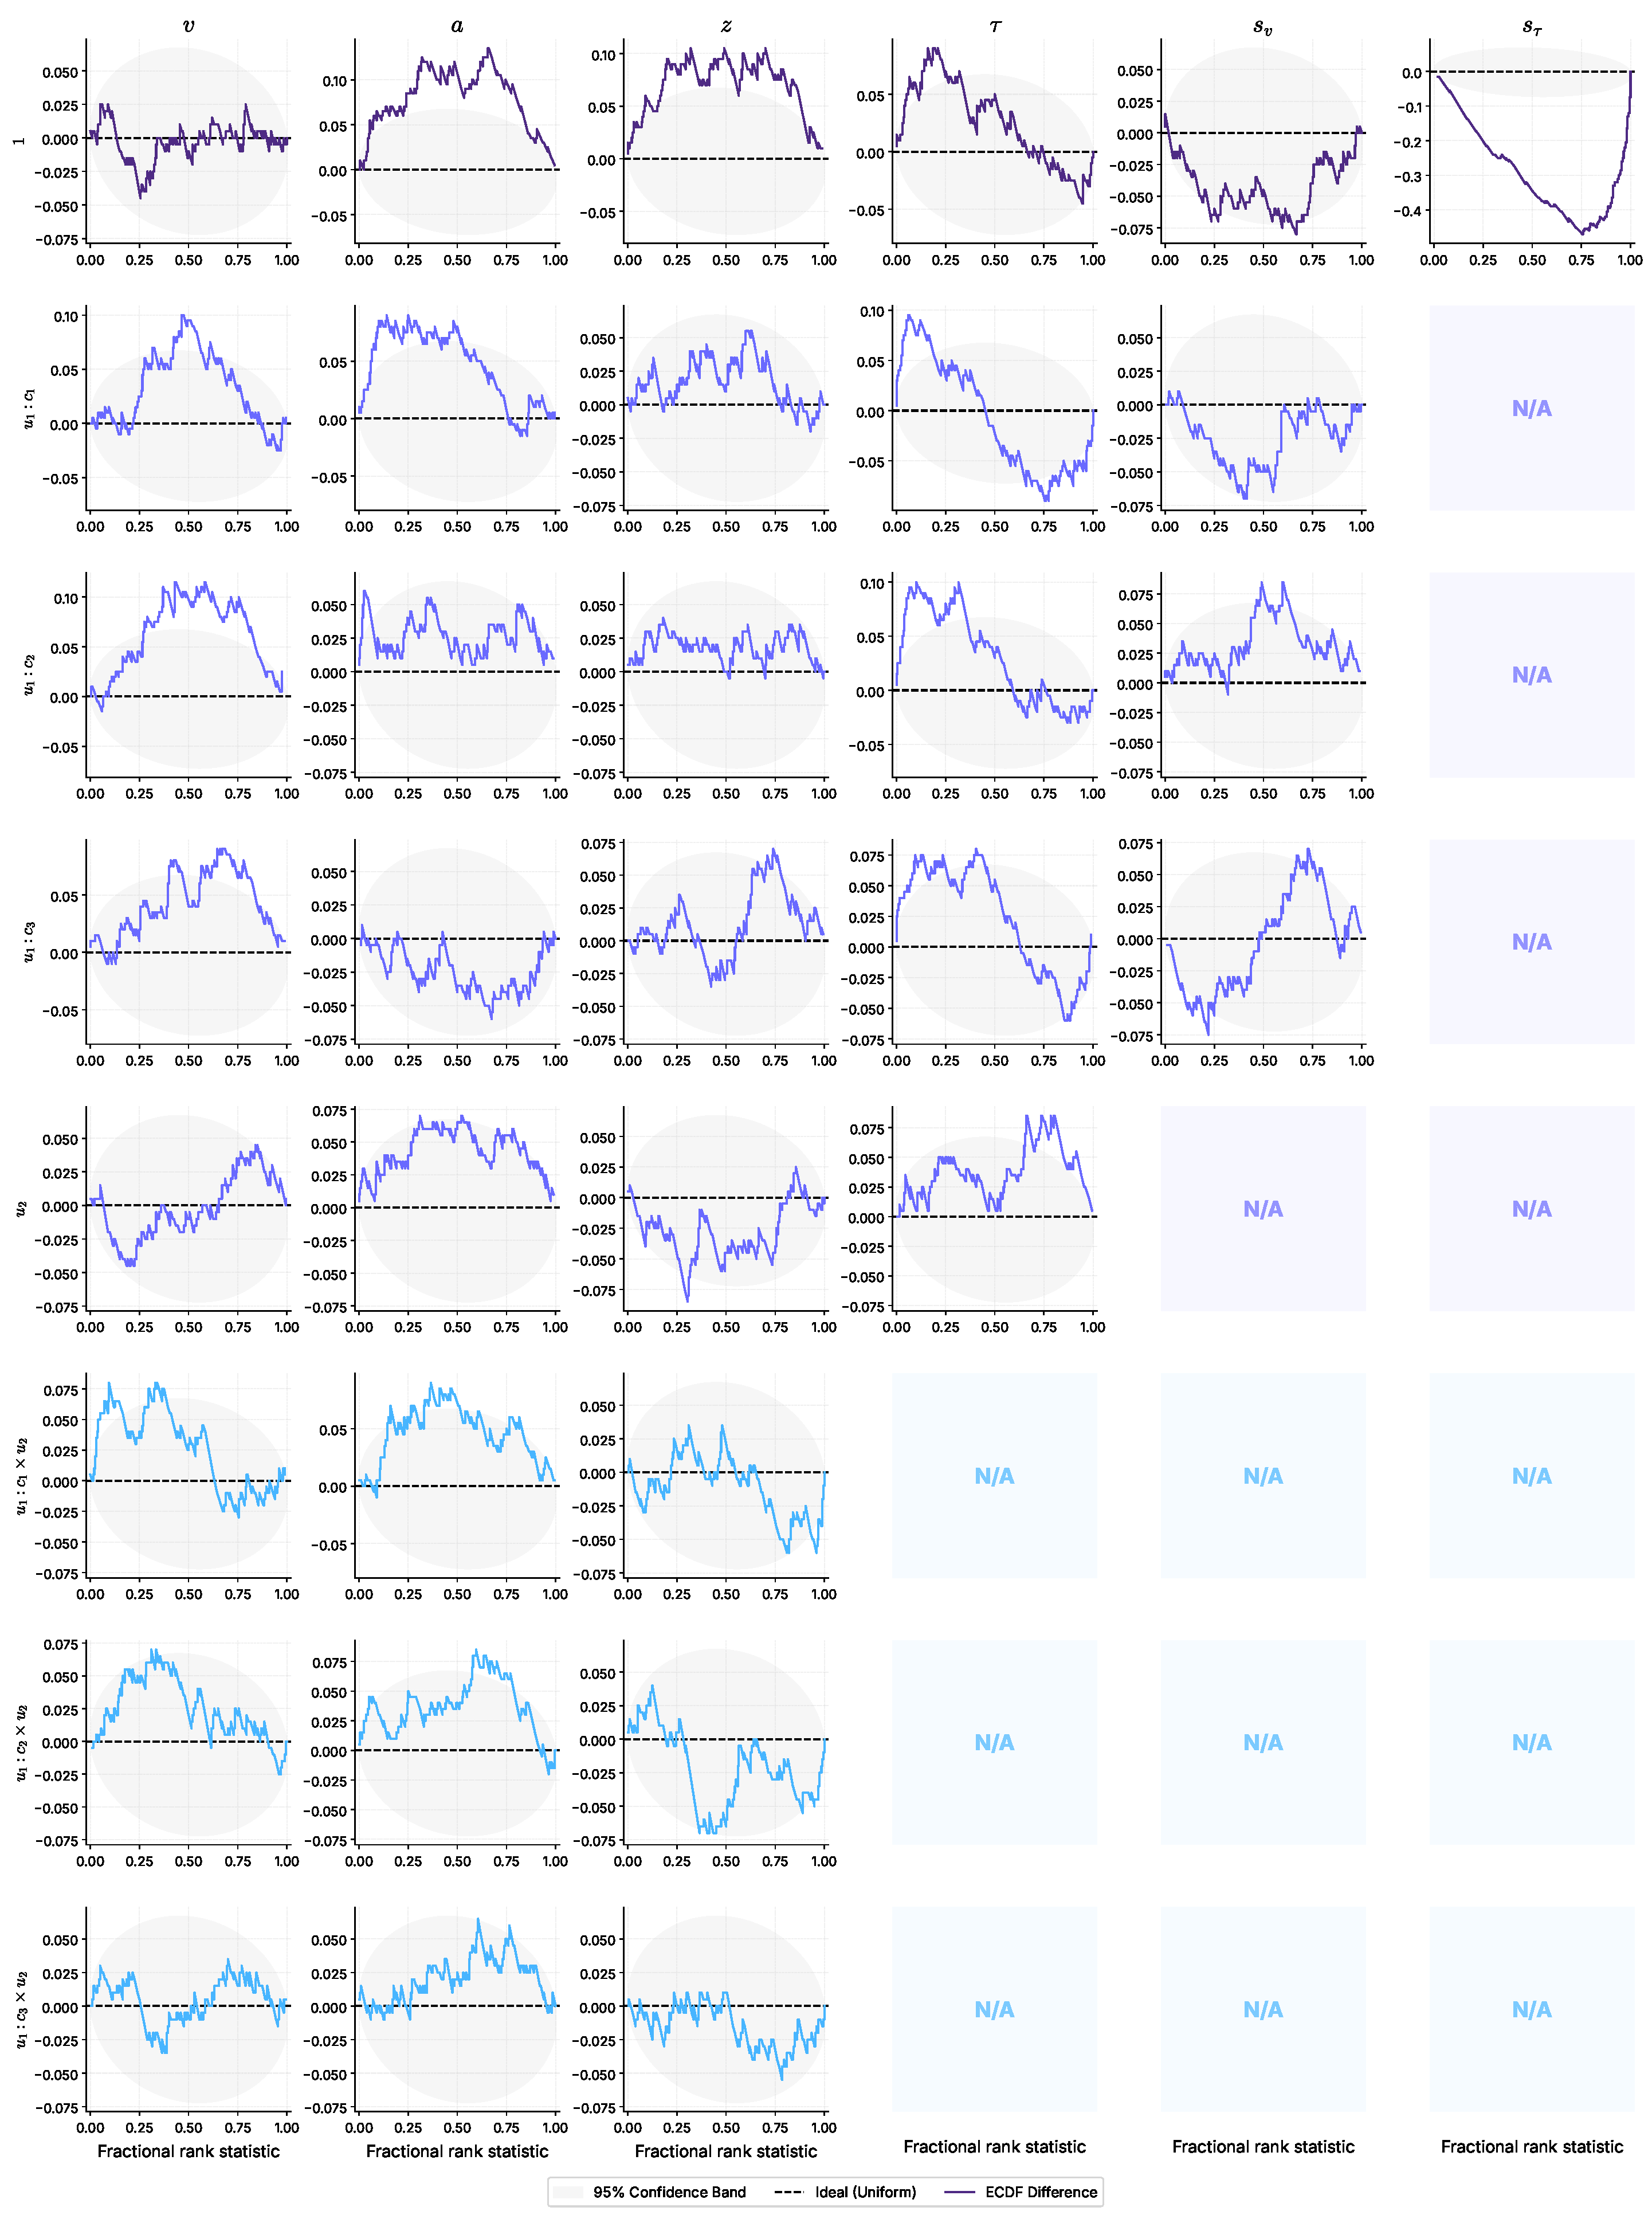
\includegraphics[width=\linewidth,height=0.84\textheight,keepaspectratio]{per_case/ddm/mixed_predictor/ecdf.pdf}
  \caption[DDM, mixed-predictor: ECDF calibration]{\textbf{DDM, mixed-predictor design --- ECDF
    calibration.} Rank-ECDF difference (empirical minus uniform) with simultaneous
    95\% confidence bands, on the same cell layout as the corresponding recovery
    figure (Figure~\ref{fig:e1-ddm-mixed_predictor-rec}). A calibrated posterior stays
    inside the band; excursions above/below indicate bias, and a systematically
    shallow/steep curve indicates over-/under-dispersion.}
  \label{fig:e1-ddm-mixed_predictor-ecdf}
\end{figure}

\FloatBarrier
\clearpage

%-----------------------------------------------------------------------------
\subsection{Racing diffusion model (RDM)}
\label{sec:e1-rdm}
%-----------------------------------------------------------------------------

Intrinsic parameters: base drift $v$, drift advantage $v_{\mathrm{diff}}$ for
the favored accumulator, threshold $a$, non-decision time $\tau$, and the
dispersions $s_v, s_\tau$.

\begin{figure}[htbp]
  \centering
  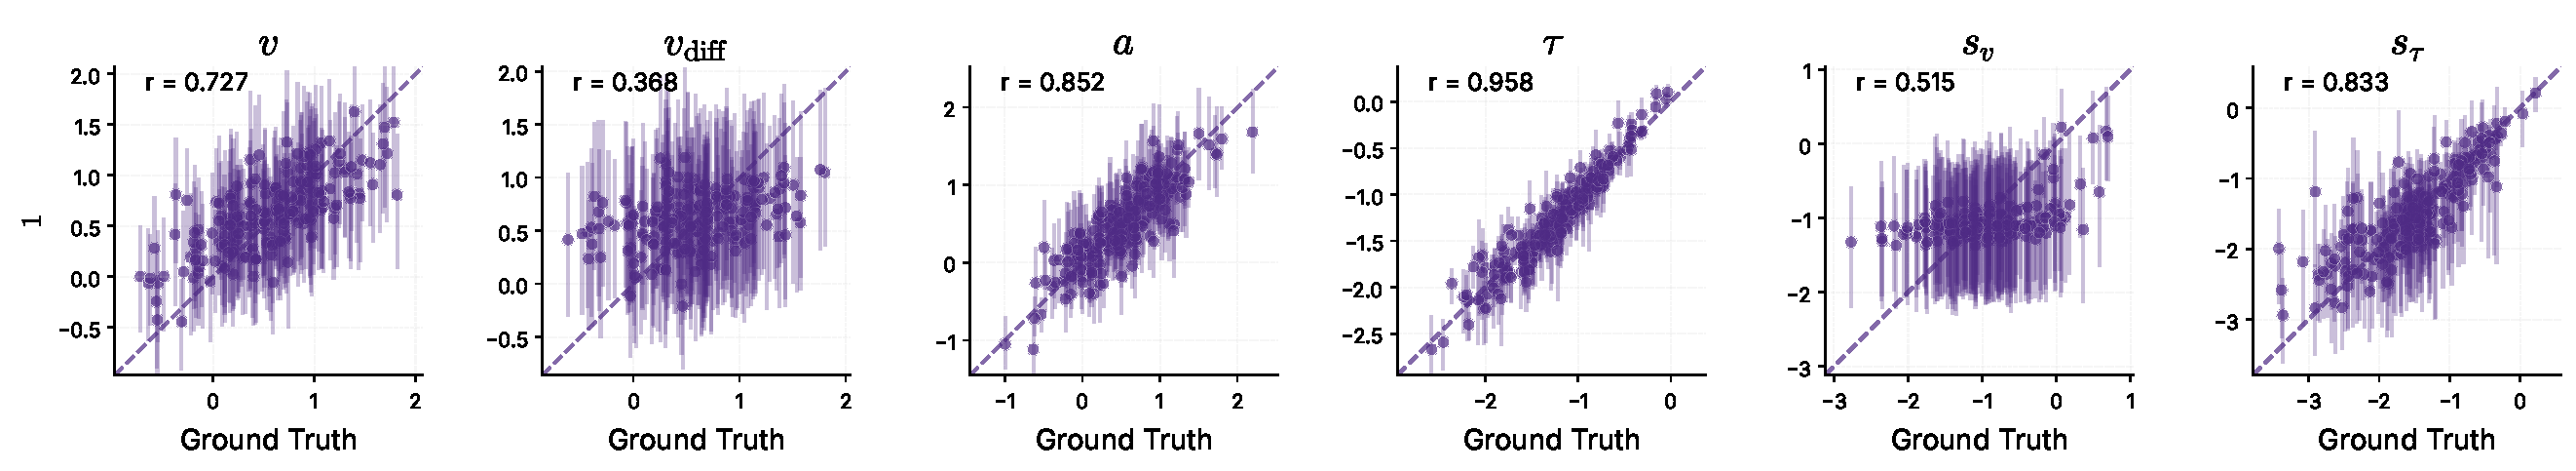
\includegraphics[width=\linewidth,height=0.84\textheight,keepaspectratio]{per_case/rdm/intercept_only/recovery.pdf}
  \caption[RDM, intercept-only: recovery]{\textbf{RDM, intercept-only design --- coefficient
    recovery.} Posterior mean (points) with 95\% credible intervals against the
    data-generating value, one panel per active cell of the coefficient matrix
    $\mathbf{B}$. Columns are intrinsic parameters, rows are design columns
    (intercept, main effects, interactions), labeled by regressor and category;
    the panel axes render this as \texttt{predictor|category}. Inactive cells are
    drawn as grey N/A tiles. Point color encodes the row kind: intercept (purple),
    main effect (blue), interaction (red).}
  \label{fig:e1-rdm-intercept_only-rec}
\end{figure}

\begin{figure}[htbp]
  \centering
  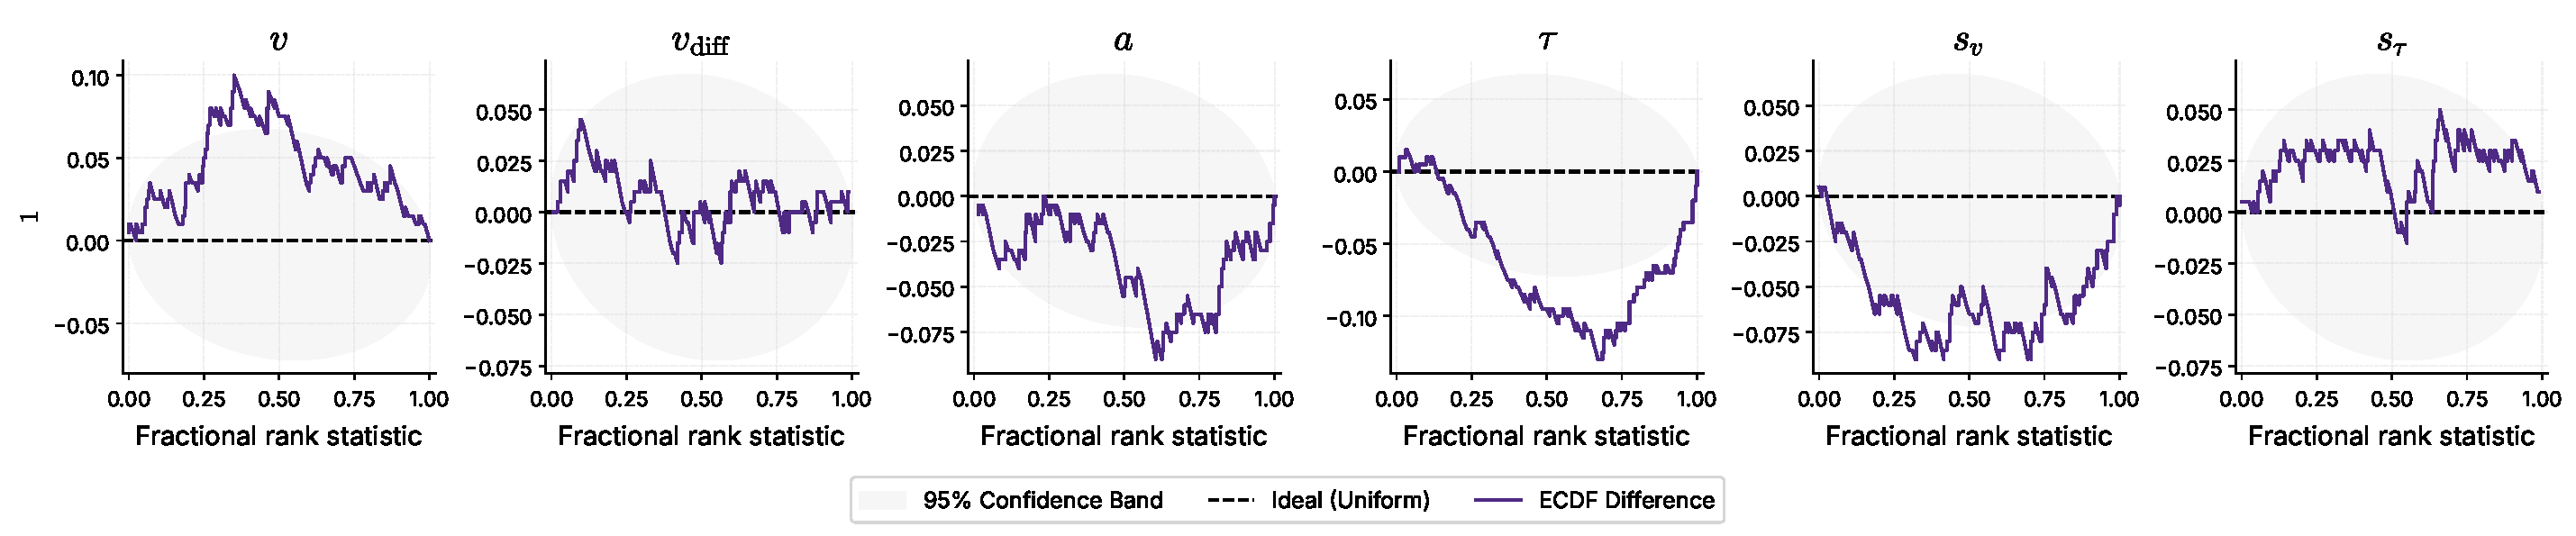
\includegraphics[width=\linewidth,height=0.84\textheight,keepaspectratio]{per_case/rdm/intercept_only/ecdf.pdf}
  \caption[RDM, intercept-only: ECDF calibration]{\textbf{RDM, intercept-only design --- ECDF
    calibration.} Rank-ECDF difference (empirical minus uniform) with simultaneous
    95\% confidence bands, on the same cell layout as the corresponding recovery
    figure (Figure~\ref{fig:e1-rdm-intercept_only-rec}). A calibrated posterior stays
    inside the band; excursions above/below indicate bias, and a systematically
    shallow/steep curve indicates over-/under-dispersion.}
  \label{fig:e1-rdm-intercept_only-ecdf}
\end{figure}

\begin{figure}[htbp]
  \centering
  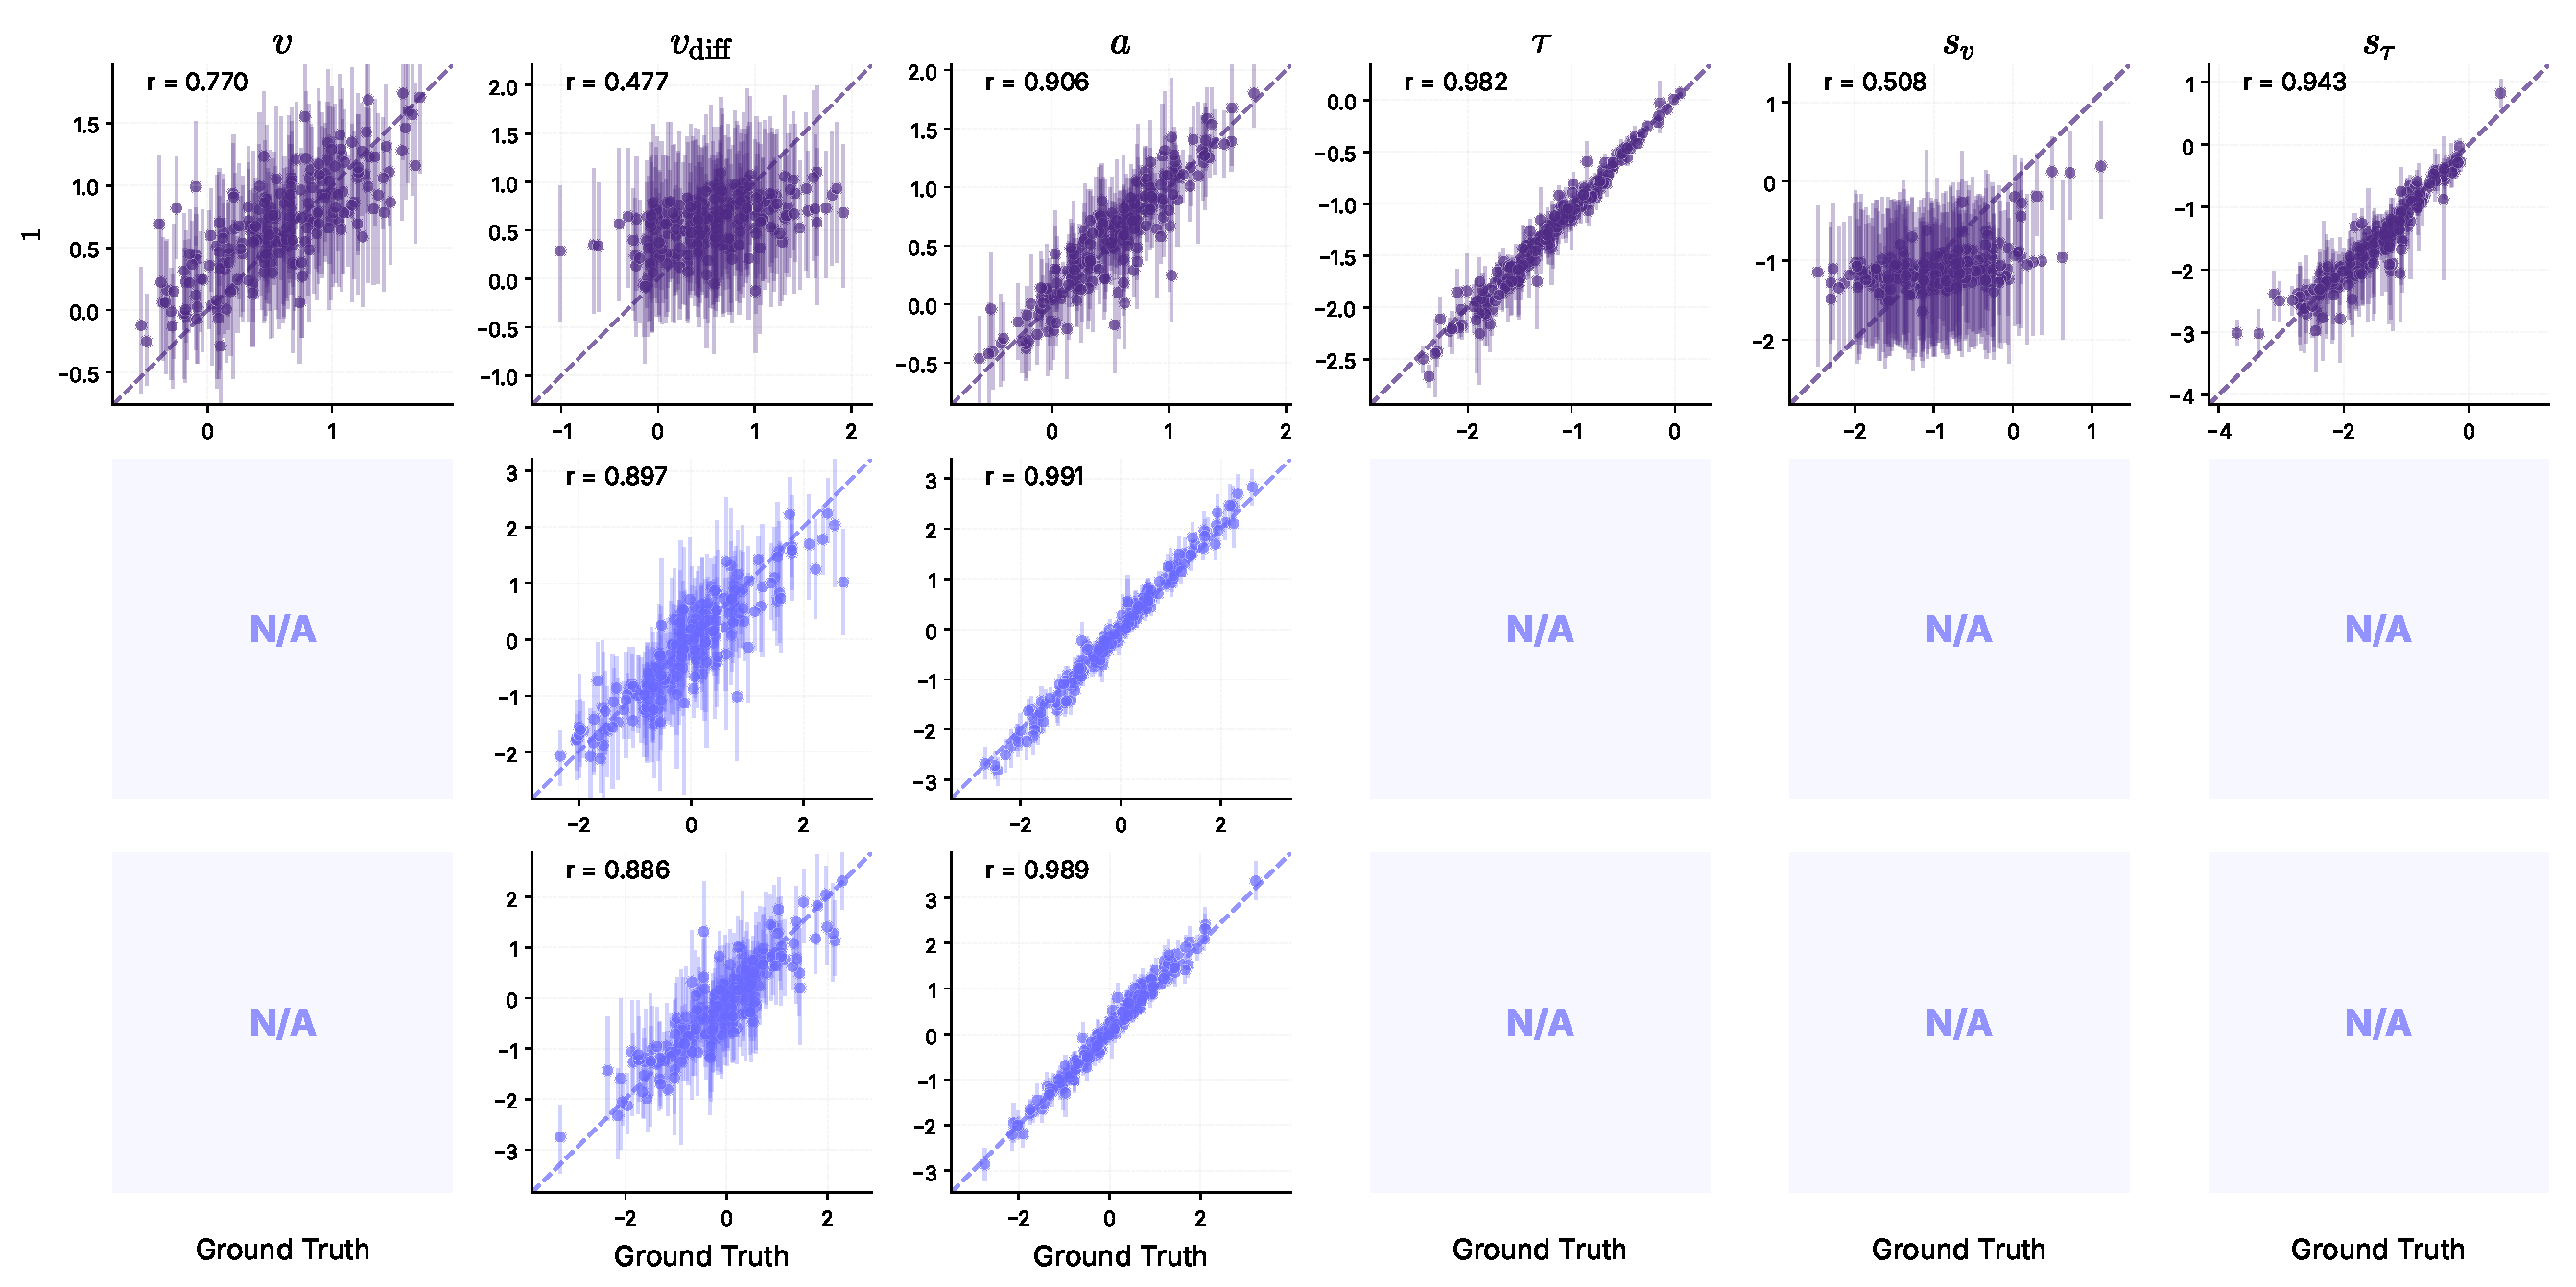
\includegraphics[width=\linewidth,height=0.84\textheight,keepaspectratio]{per_case/rdm/regressed/recovery.pdf}
  \caption[RDM, regressed: recovery]{\textbf{RDM, regressed design --- coefficient
    recovery.} Posterior mean (points) with 95\% credible intervals against the
    data-generating value, one panel per active cell of the coefficient matrix
    $\mathbf{B}$. Columns are intrinsic parameters, rows are design columns
    (intercept, main effects, interactions), labeled by regressor and category;
    the panel axes render this as \texttt{predictor|category}. Inactive cells are
    drawn as grey N/A tiles. Point color encodes the row kind: intercept (purple),
    main effect (blue), interaction (red).}
  \label{fig:e1-rdm-regressed-rec}
\end{figure}

\begin{figure}[htbp]
  \centering
  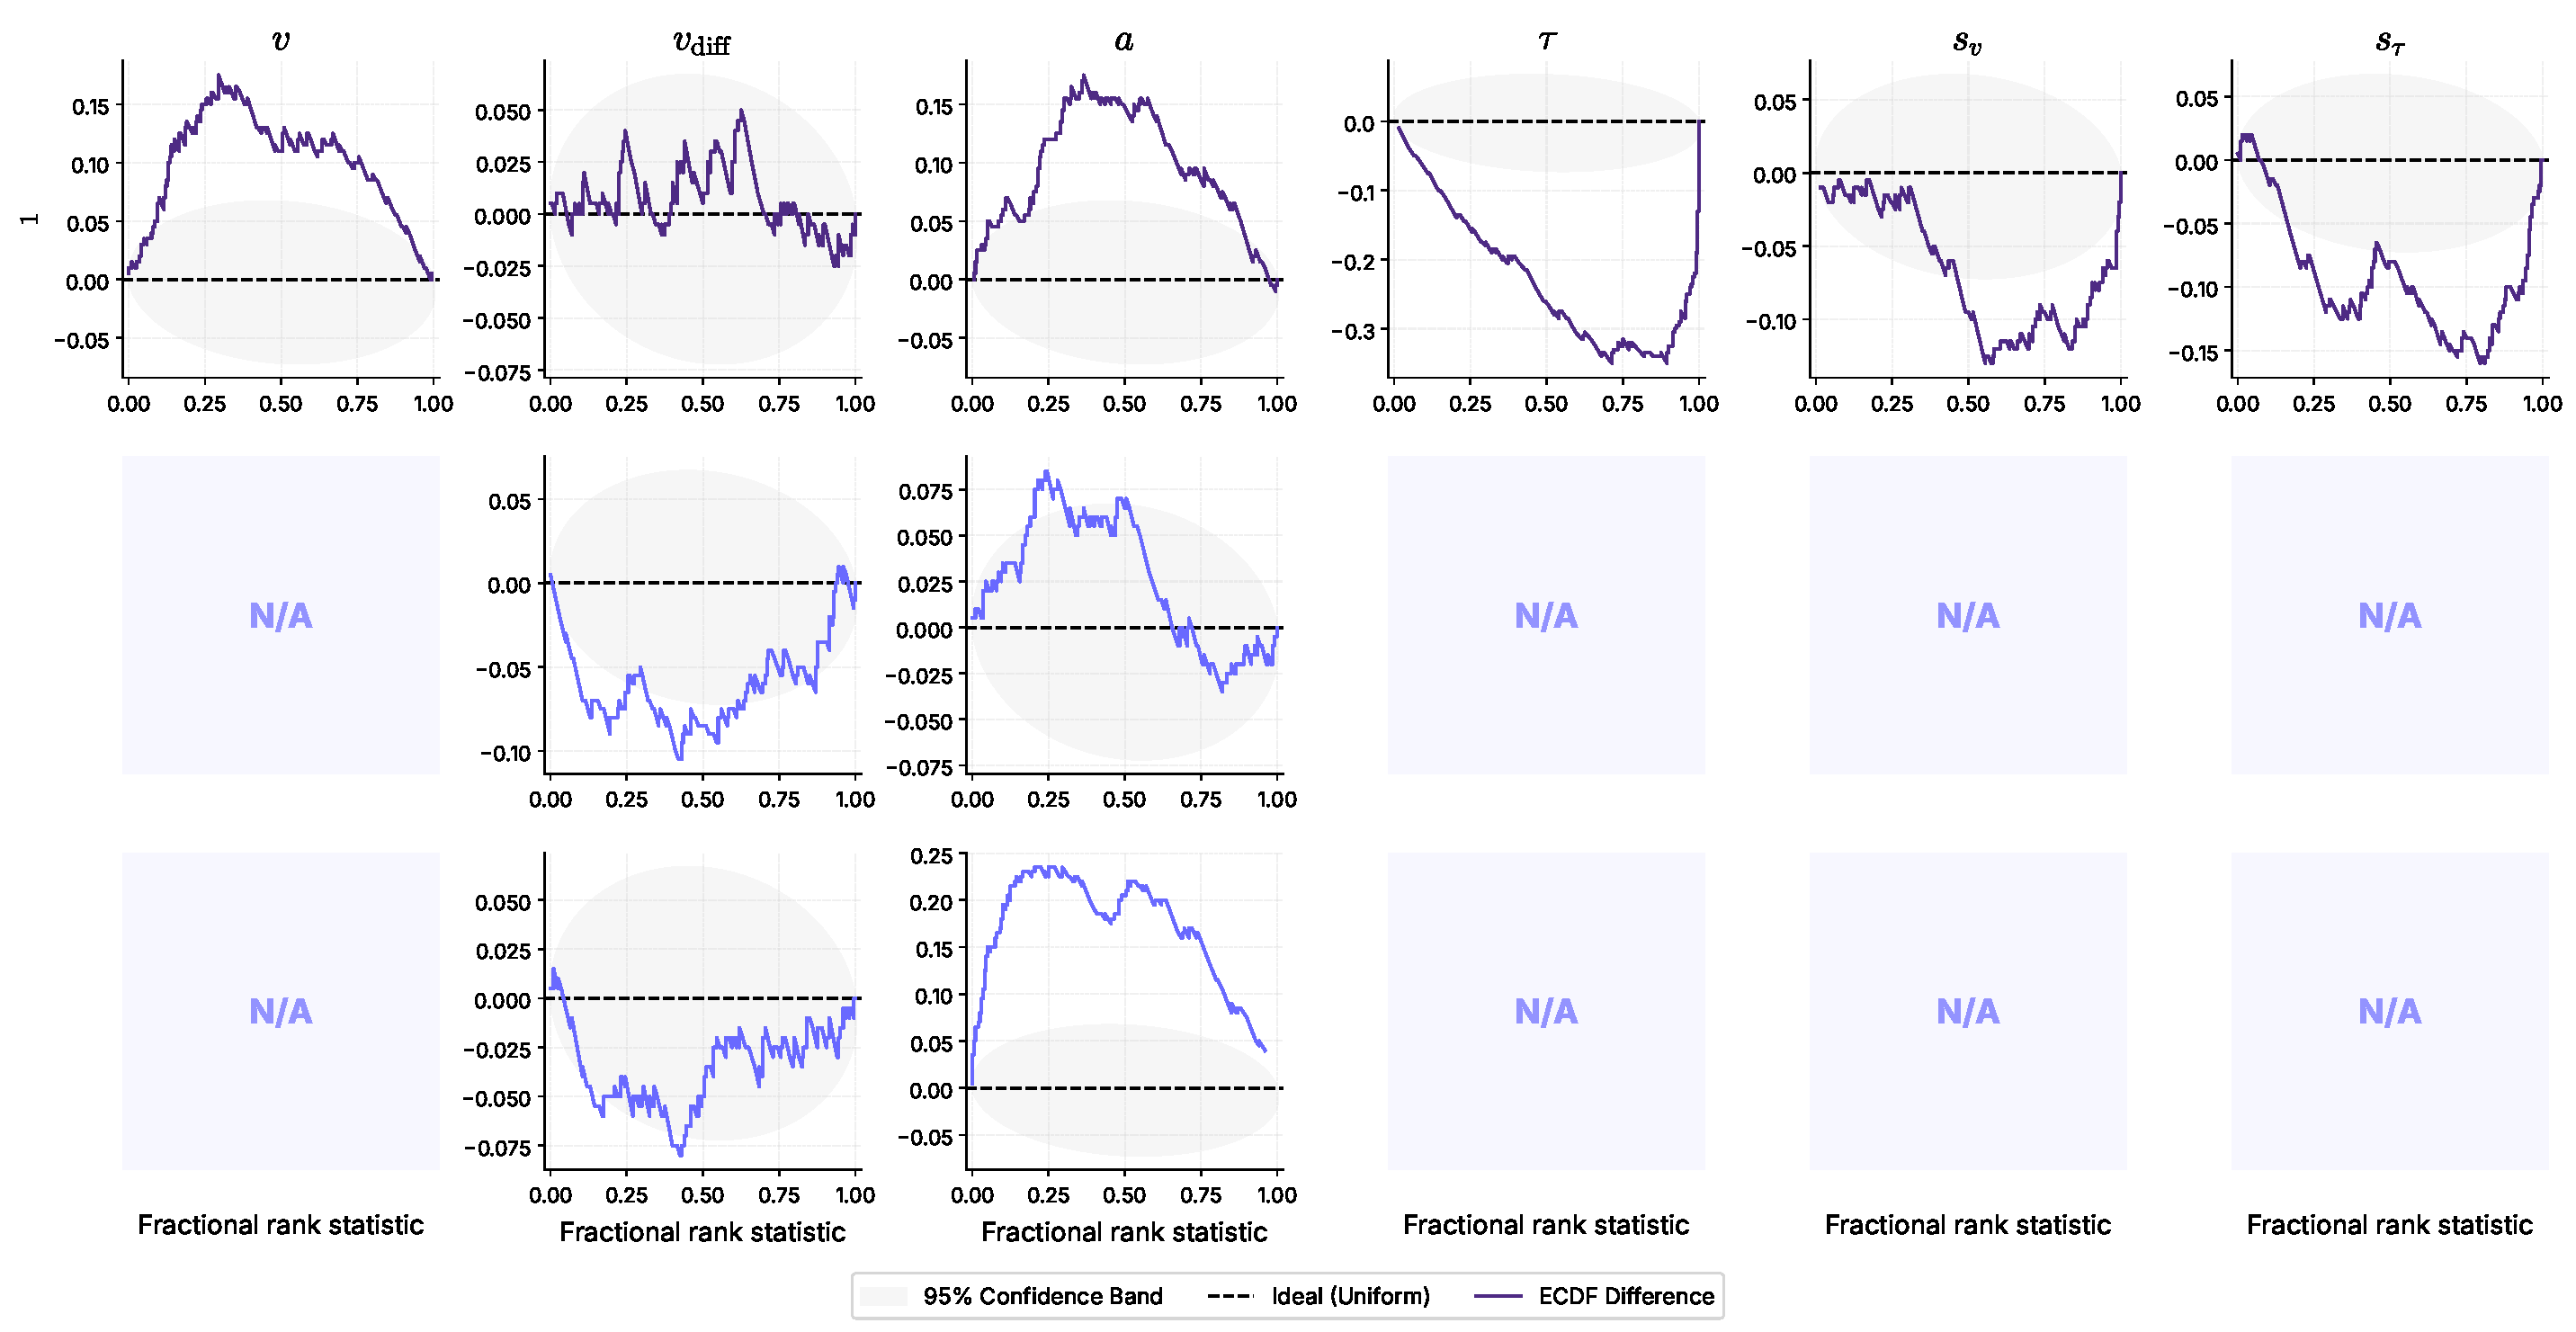
\includegraphics[width=\linewidth,height=0.84\textheight,keepaspectratio]{per_case/rdm/regressed/ecdf.pdf}
  \caption[RDM, regressed: ECDF calibration]{\textbf{RDM, regressed design --- ECDF
    calibration.} Rank-ECDF difference (empirical minus uniform) with simultaneous
    95\% confidence bands, on the same cell layout as the corresponding recovery
    figure (Figure~\ref{fig:e1-rdm-regressed-rec}). A calibrated posterior stays
    inside the band; excursions above/below indicate bias, and a systematically
    shallow/steep curve indicates over-/under-dispersion.}
  \label{fig:e1-rdm-regressed-ecdf}
\end{figure}

\begin{figure}[htbp]
  \centering
  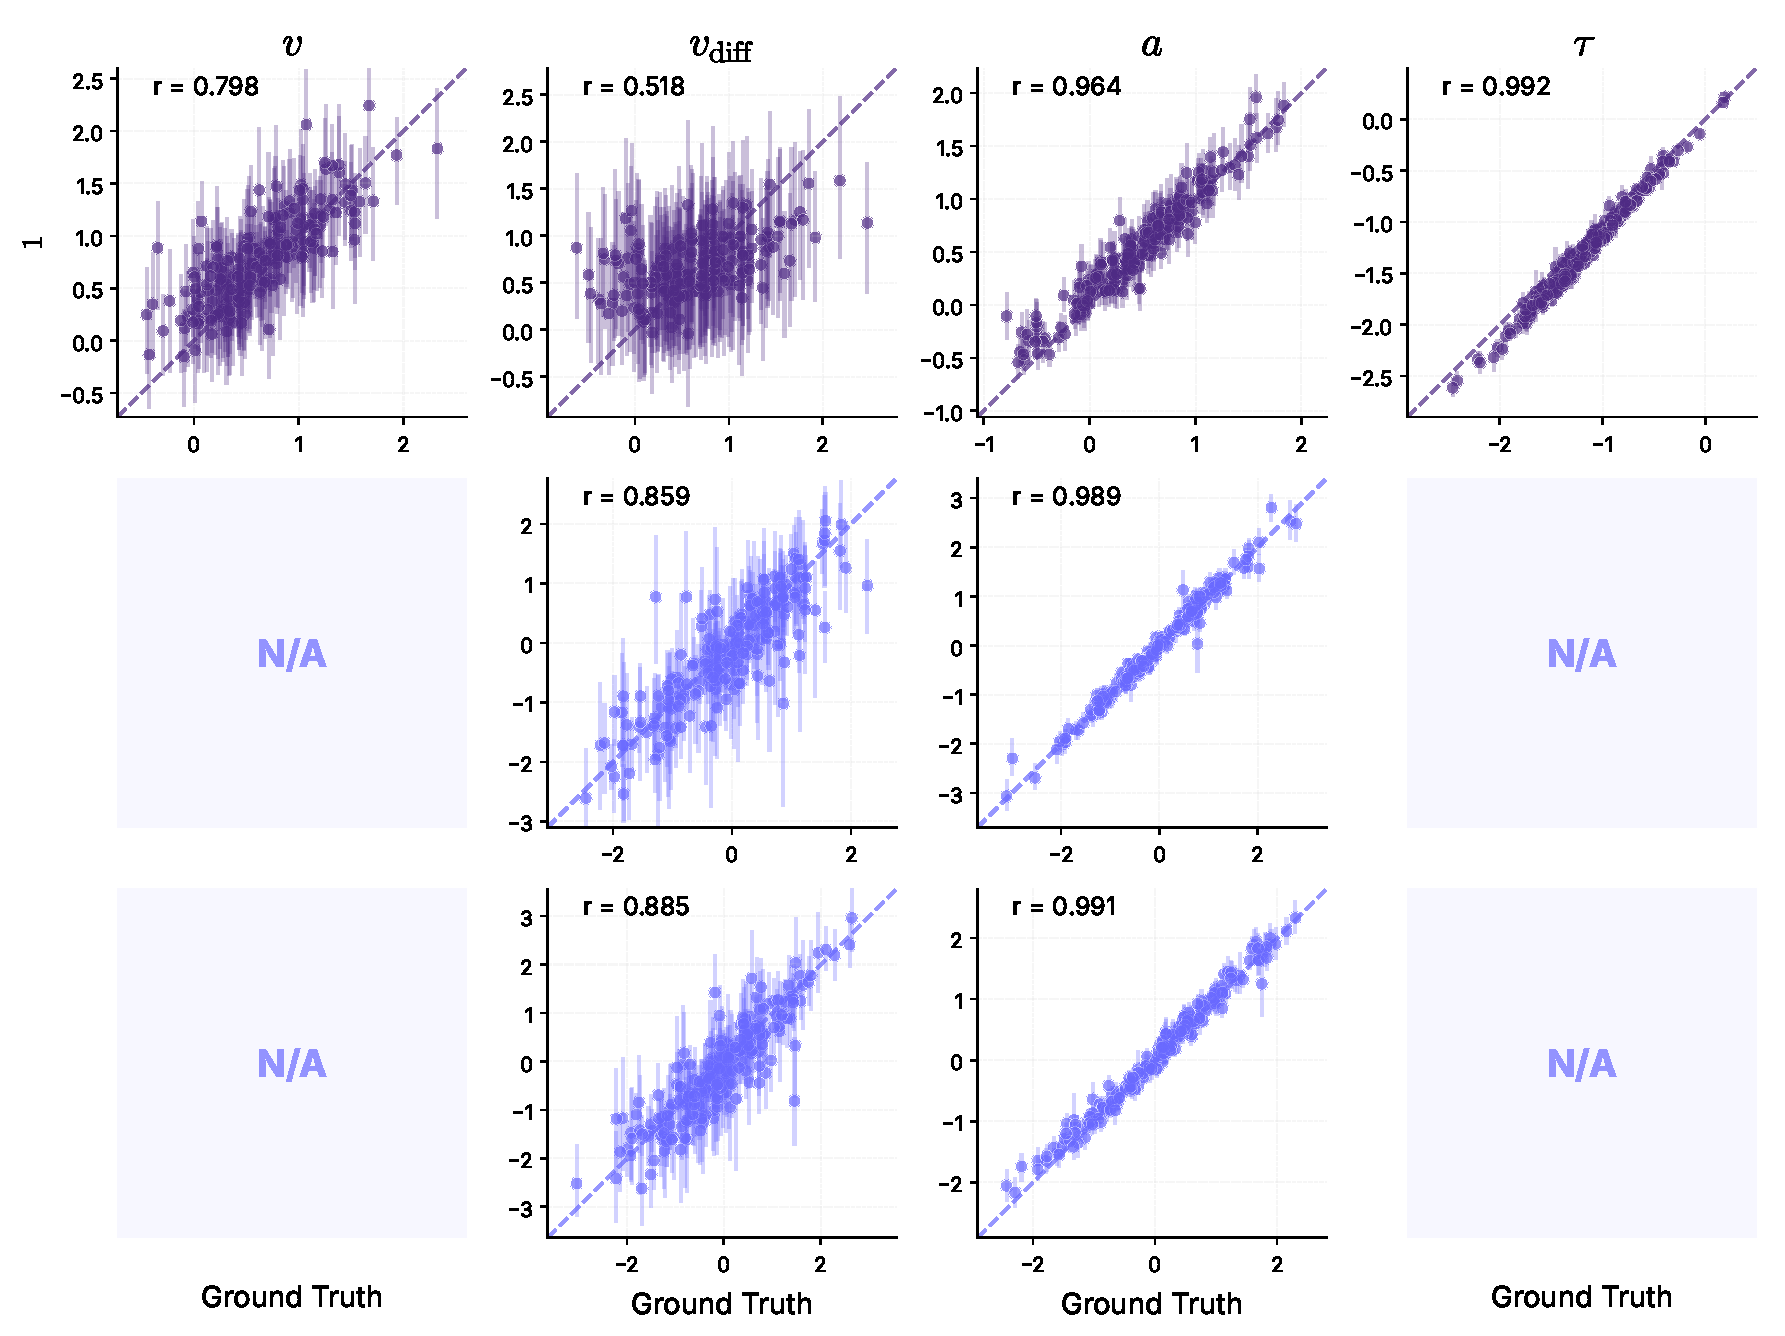
\includegraphics[width=\linewidth,height=0.84\textheight,keepaspectratio]{per_case/rdm/fixed_regressed/recovery.pdf}
  \caption[RDM, fixed-regressed: recovery]{\textbf{RDM, fixed-regressed design --- coefficient
    recovery.} Posterior mean (points) with 95\% credible intervals against the
    data-generating value, one panel per active cell of the coefficient matrix
    $\mathbf{B}$. Columns are intrinsic parameters, rows are design columns
    (intercept, main effects, interactions), labeled by regressor and category;
    the panel axes render this as \texttt{predictor|category}. Inactive cells are
    drawn as grey N/A tiles. Point color encodes the row kind: intercept (purple),
    main effect (blue), interaction (red).}
  \label{fig:e1-rdm-fixed_regressed-rec}
\end{figure}

\begin{figure}[htbp]
  \centering
  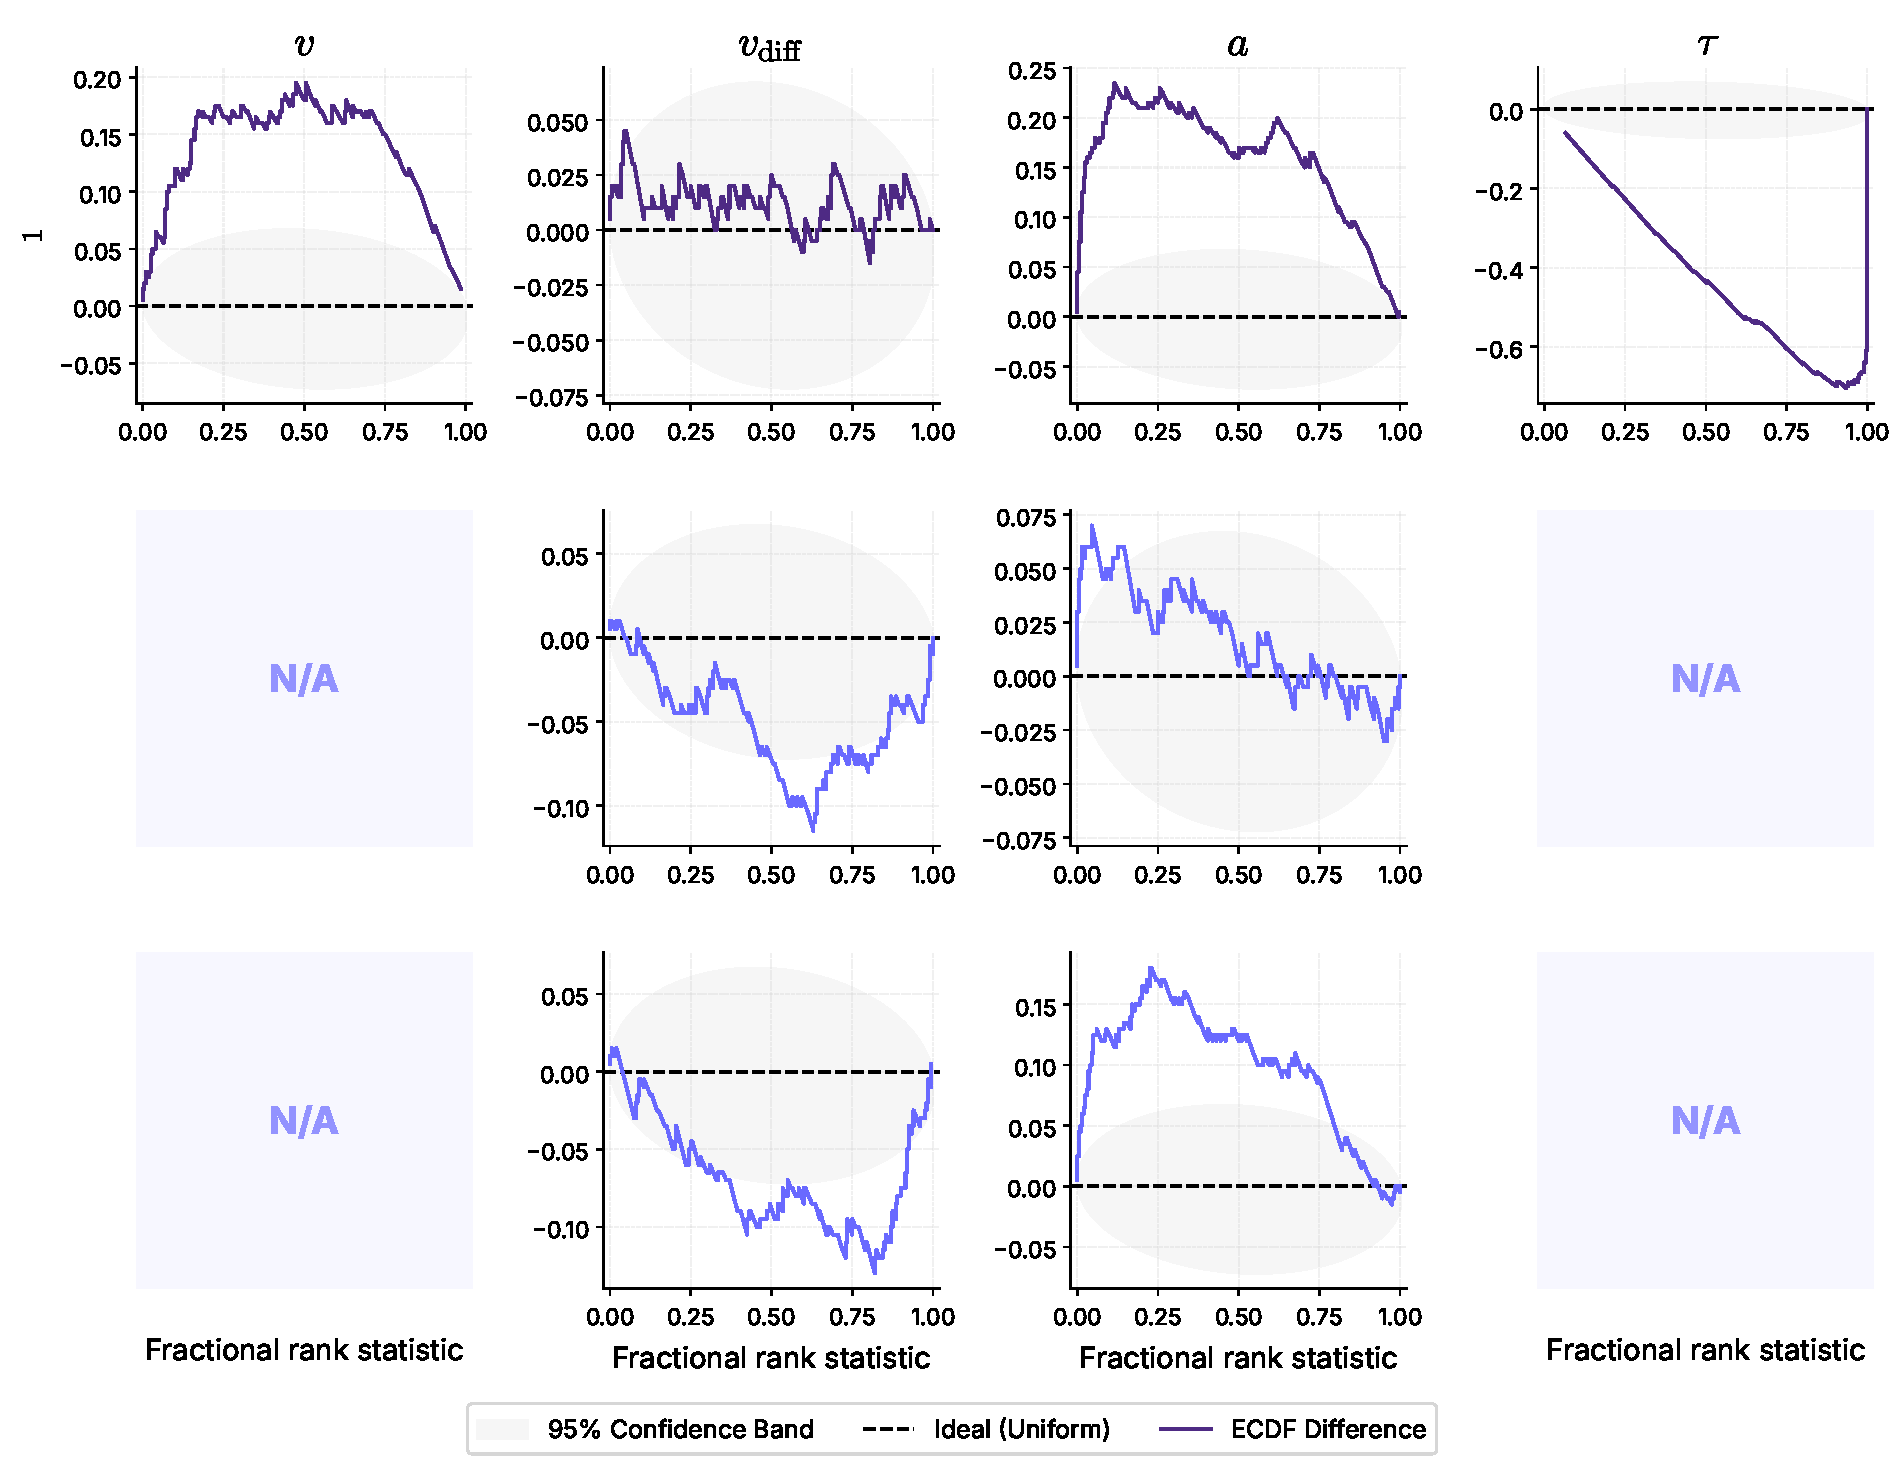
\includegraphics[width=\linewidth,height=0.84\textheight,keepaspectratio]{per_case/rdm/fixed_regressed/ecdf.pdf}
  \caption[RDM, fixed-regressed: ECDF calibration]{\textbf{RDM, fixed-regressed design --- ECDF
    calibration.} Rank-ECDF difference (empirical minus uniform) with simultaneous
    95\% confidence bands, on the same cell layout as the corresponding recovery
    figure (Figure~\ref{fig:e1-rdm-fixed_regressed-rec}). A calibrated posterior stays
    inside the band; excursions above/below indicate bias, and a systematically
    shallow/steep curve indicates over-/under-dispersion.}
  \label{fig:e1-rdm-fixed_regressed-ecdf}
\end{figure}

\begin{figure}[htbp]
  \centering
  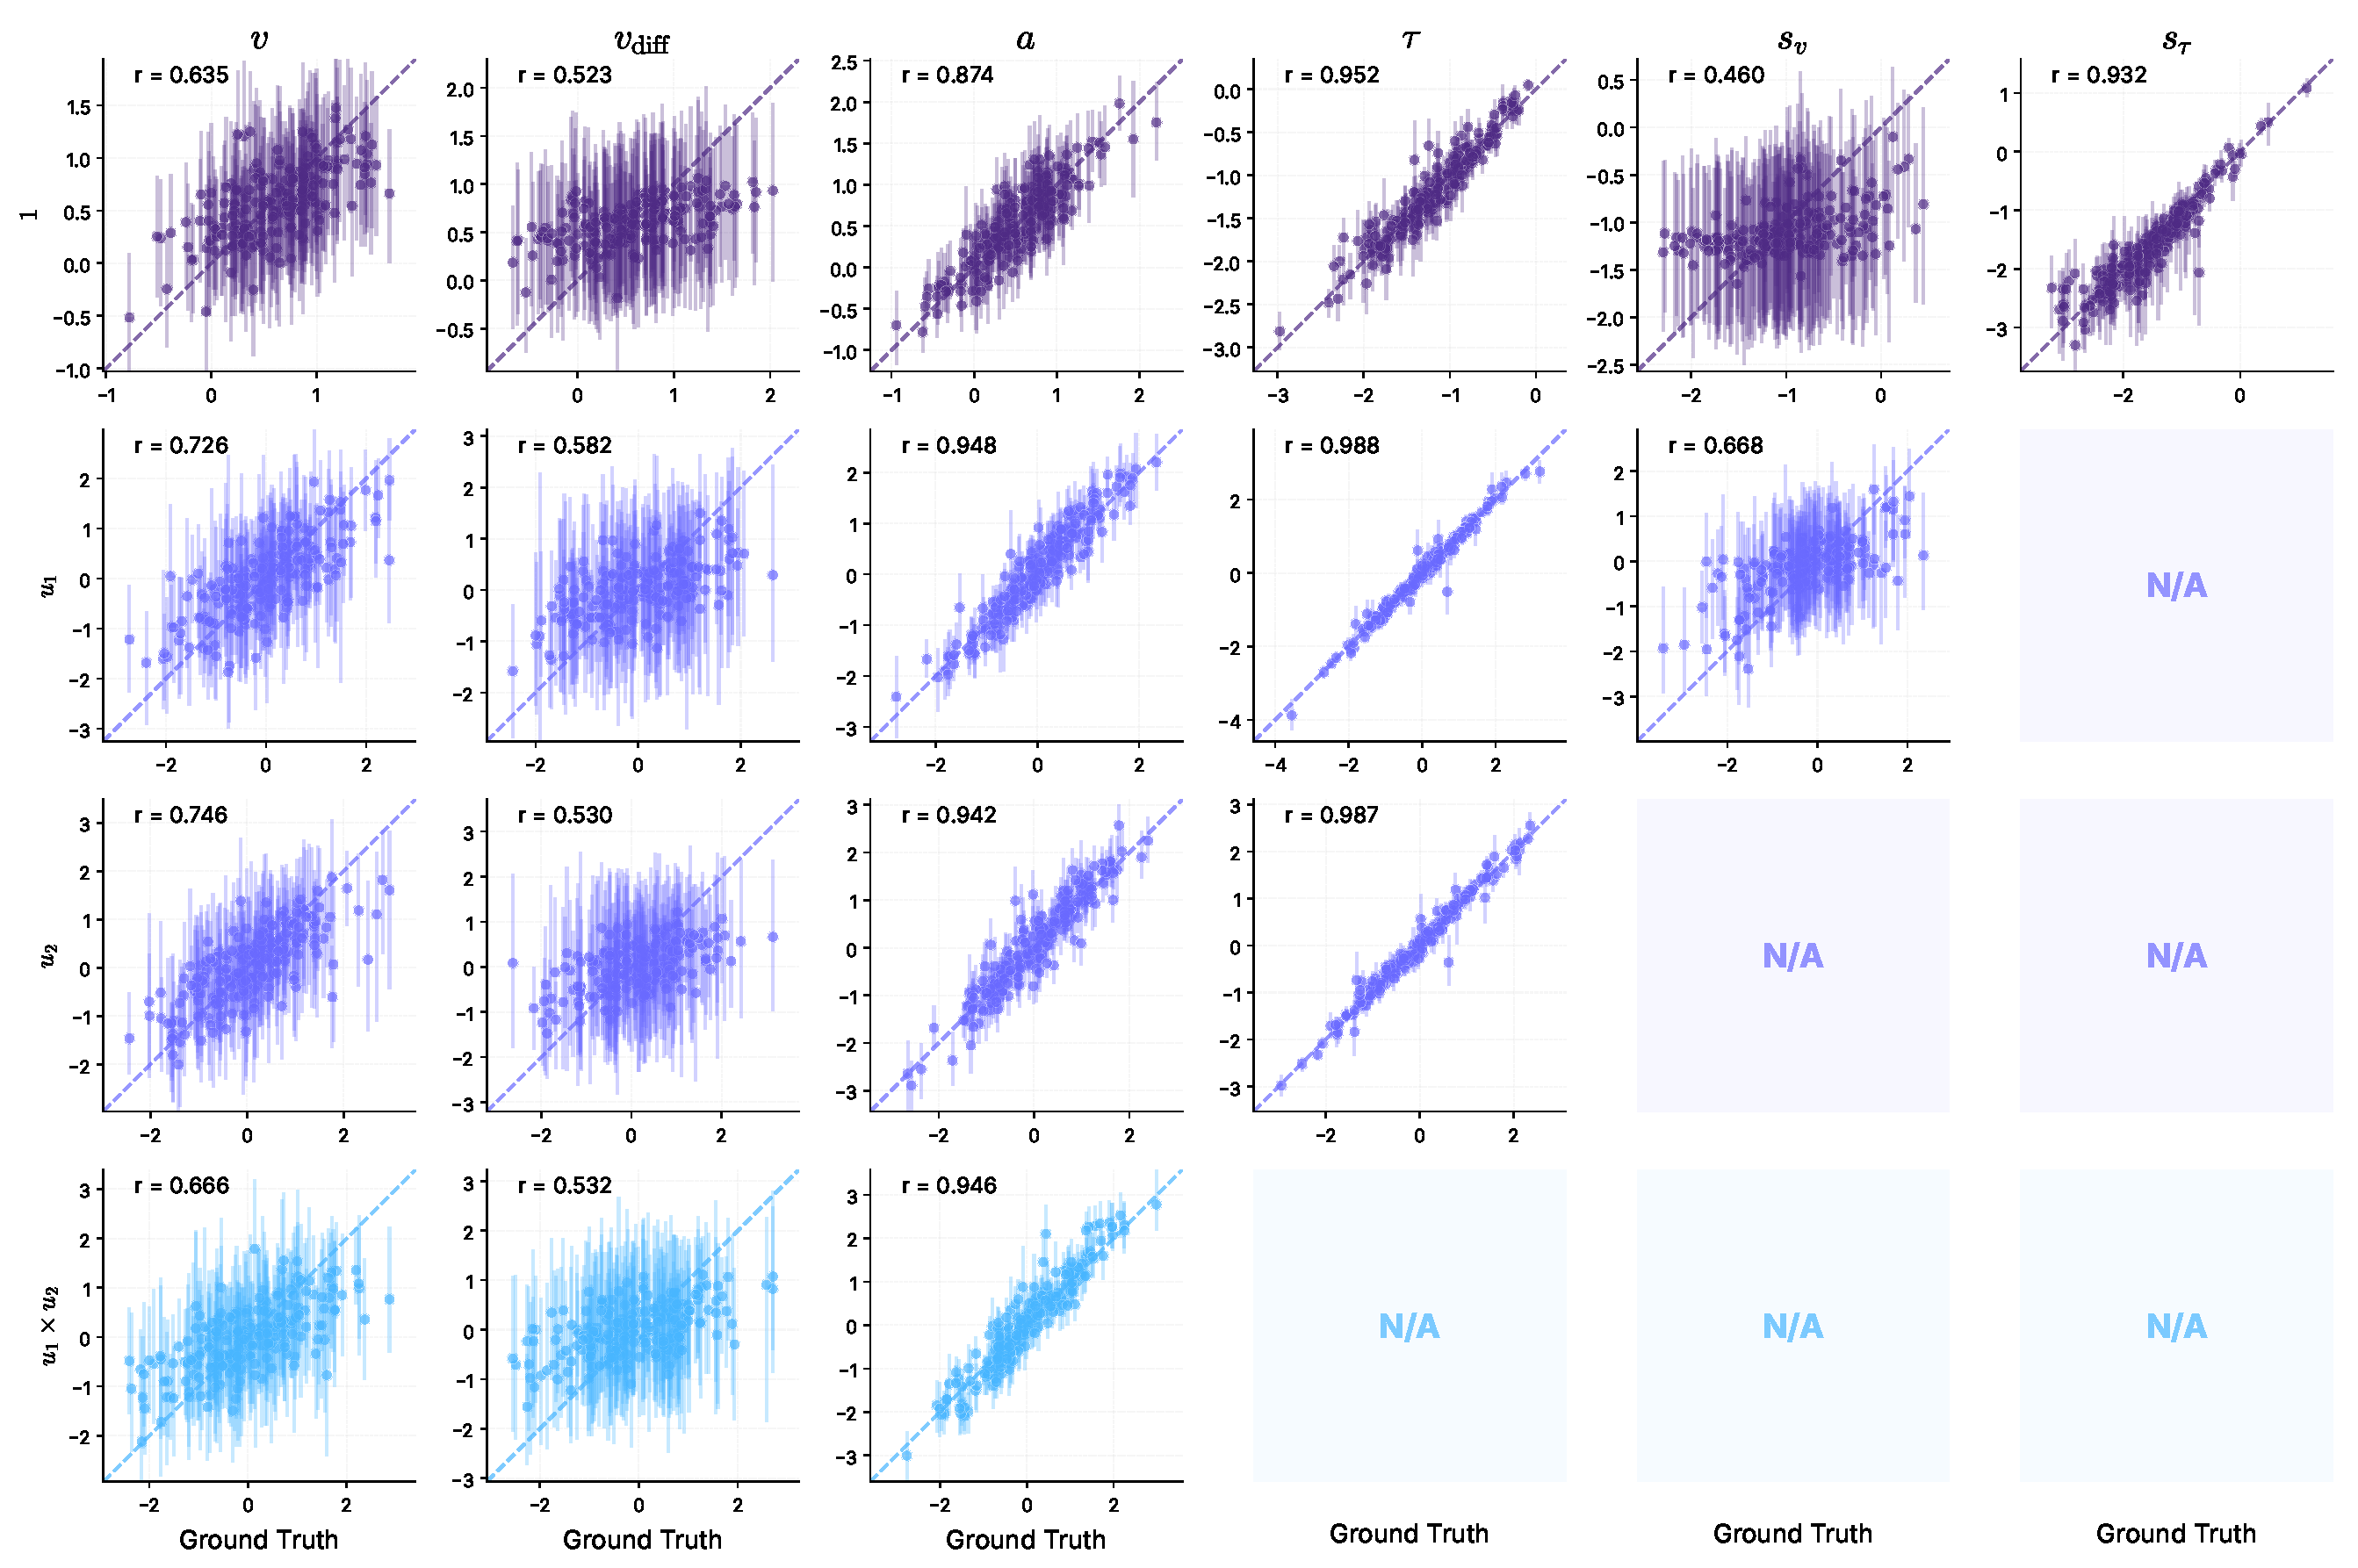
\includegraphics[width=\linewidth,height=0.84\textheight,keepaspectratio]{per_case/rdm/interaction/recovery.pdf}
  \caption[RDM, interaction: recovery]{\textbf{RDM, interaction design --- coefficient
    recovery.} Posterior mean (points) with 95\% credible intervals against the
    data-generating value, one panel per active cell of the coefficient matrix
    $\mathbf{B}$. Columns are intrinsic parameters, rows are design columns
    (intercept, main effects, interactions), labeled by regressor and category;
    the panel axes render this as \texttt{predictor|category}. Inactive cells are
    drawn as grey N/A tiles. Point color encodes the row kind: intercept (purple),
    main effect (blue), interaction (red).}
  \label{fig:e1-rdm-interaction-rec}
\end{figure}

\begin{figure}[htbp]
  \centering
  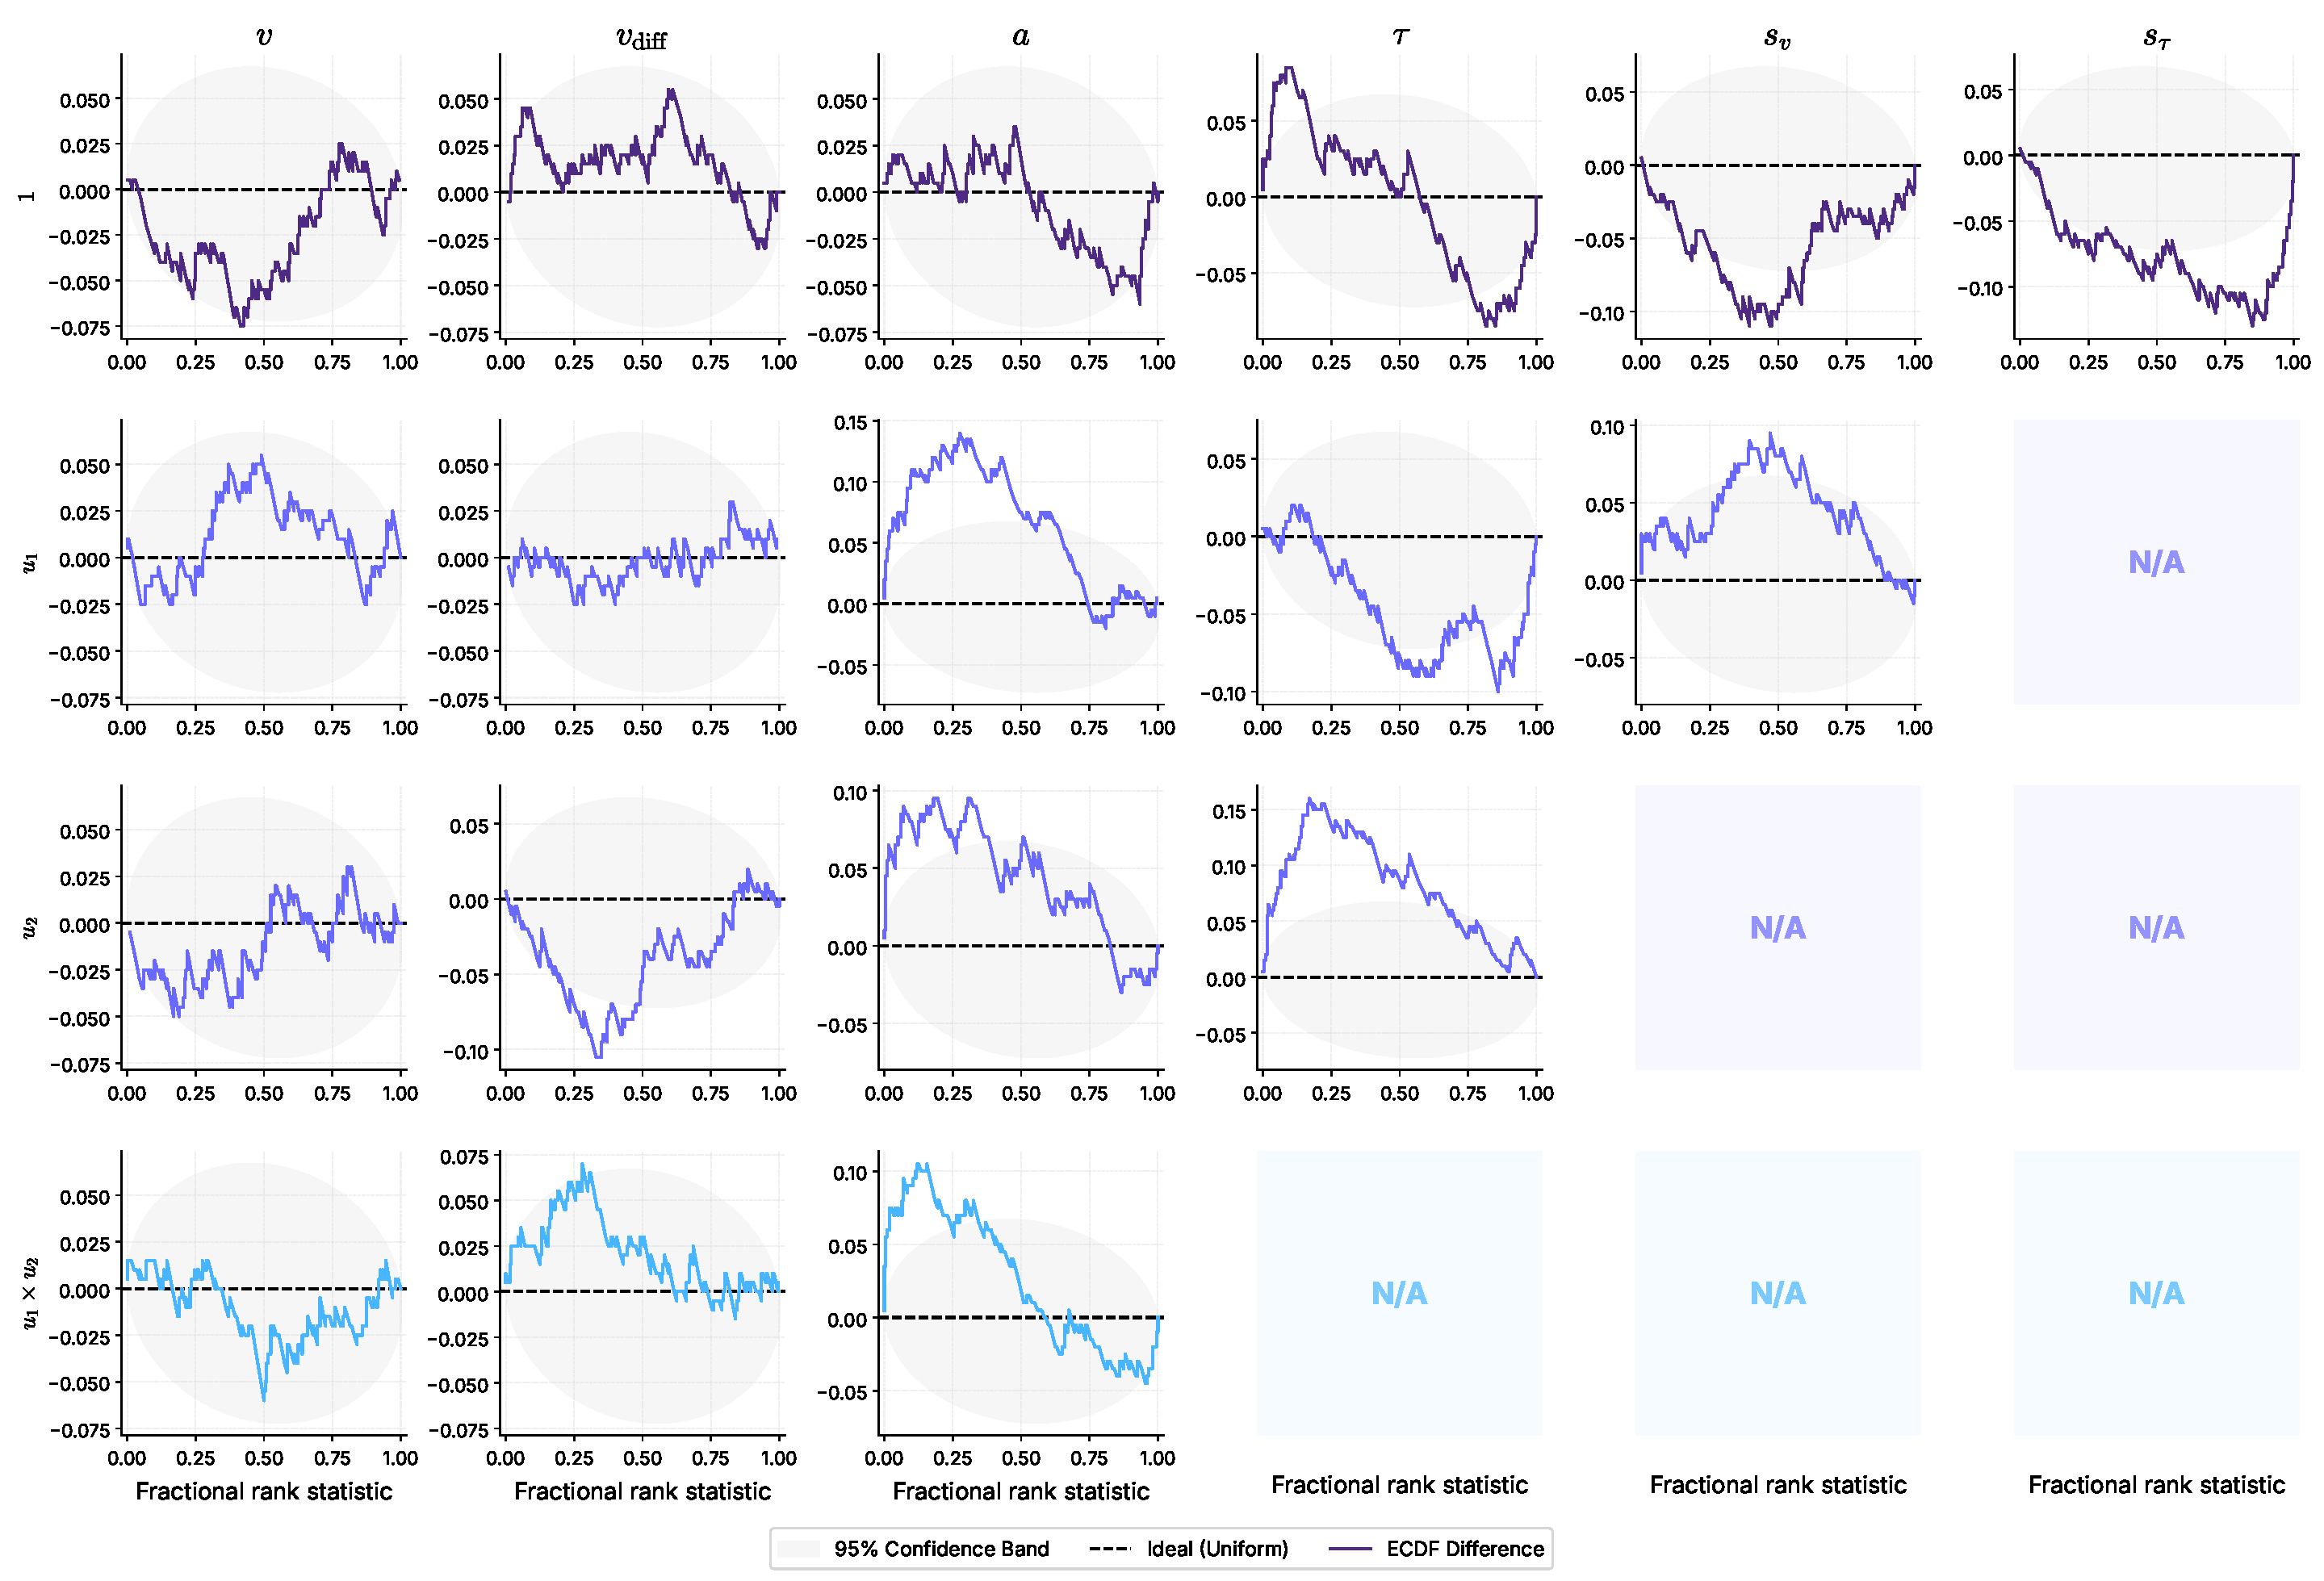
\includegraphics[width=\linewidth,height=0.84\textheight,keepaspectratio]{per_case/rdm/interaction/ecdf.pdf}
  \caption[RDM, interaction: ECDF calibration]{\textbf{RDM, interaction design --- ECDF
    calibration.} Rank-ECDF difference (empirical minus uniform) with simultaneous
    95\% confidence bands, on the same cell layout as the corresponding recovery
    figure (Figure~\ref{fig:e1-rdm-interaction-rec}). A calibrated posterior stays
    inside the band; excursions above/below indicate bias, and a systematically
    shallow/steep curve indicates over-/under-dispersion.}
  \label{fig:e1-rdm-interaction-ecdf}
\end{figure}

\begin{figure}[htbp]
  \centering
  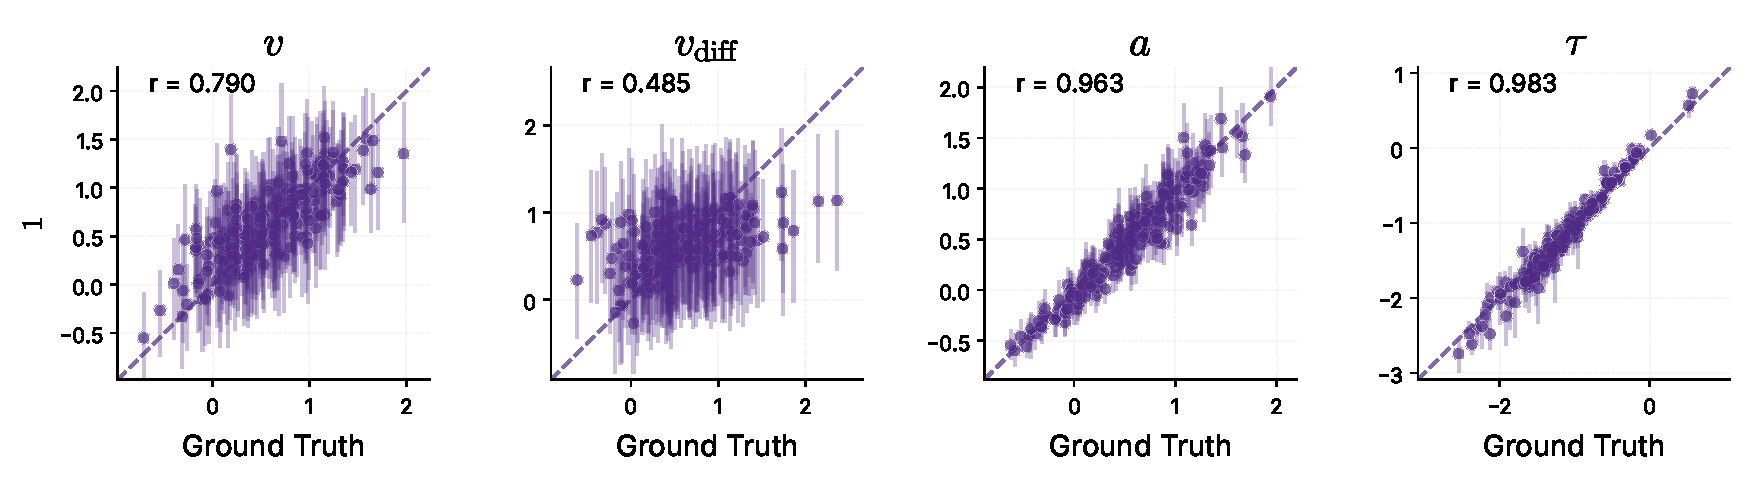
\includegraphics[width=\linewidth,height=0.84\textheight,keepaspectratio]{per_case/rdm/fixed/recovery.pdf}
  \caption[RDM, fixed: recovery]{\textbf{RDM, fixed design --- coefficient
    recovery.} Posterior mean (points) with 95\% credible intervals against the
    data-generating value, one panel per active cell of the coefficient matrix
    $\mathbf{B}$. Columns are intrinsic parameters, rows are design columns
    (intercept, main effects, interactions), labeled by regressor and category;
    the panel axes render this as \texttt{predictor|category}. Inactive cells are
    drawn as grey N/A tiles. Point color encodes the row kind: intercept (purple),
    main effect (blue), interaction (red).}
  \label{fig:e1-rdm-fixed-rec}
\end{figure}

\begin{figure}[htbp]
  \centering
  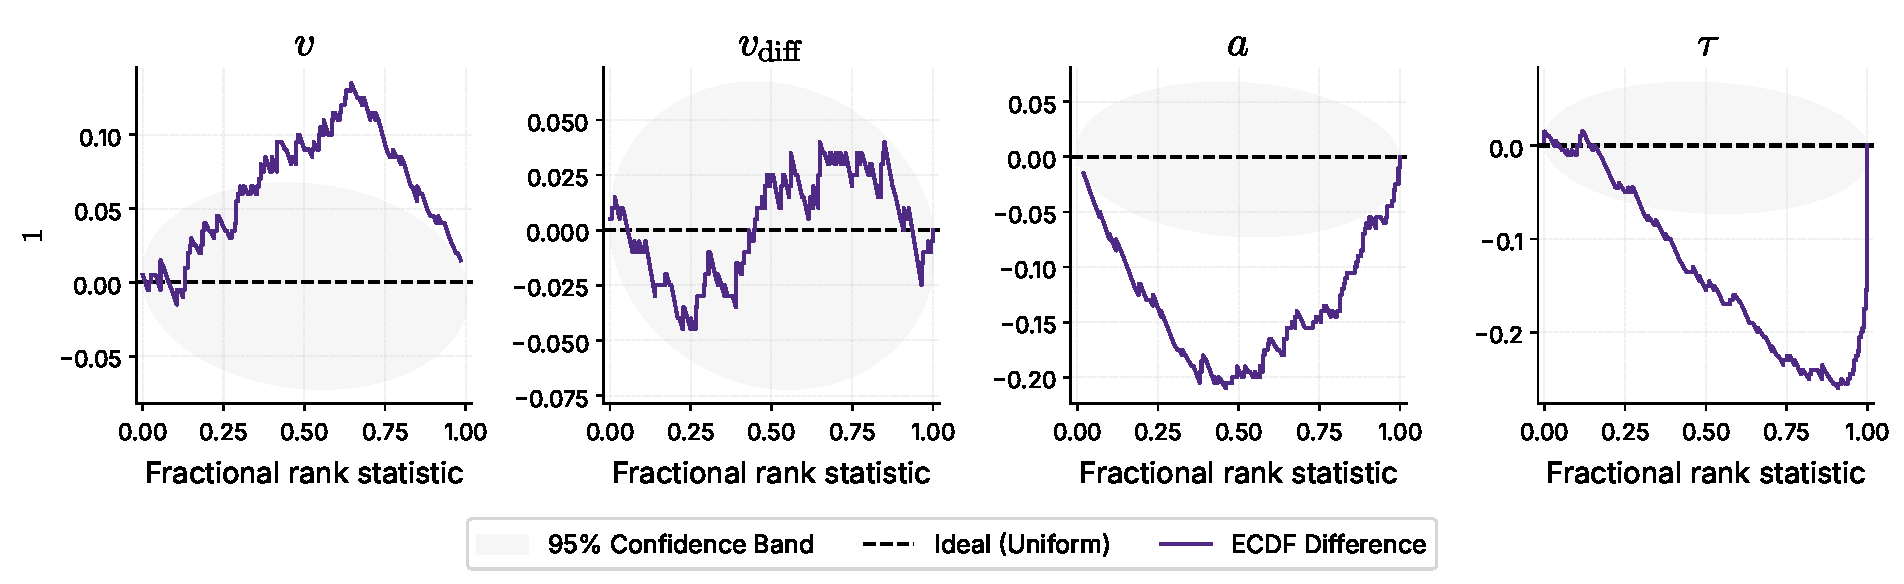
\includegraphics[width=\linewidth,height=0.84\textheight,keepaspectratio]{per_case/rdm/fixed/ecdf.pdf}
  \caption[RDM, fixed: ECDF calibration]{\textbf{RDM, fixed design --- ECDF
    calibration.} Rank-ECDF difference (empirical minus uniform) with simultaneous
    95\% confidence bands, on the same cell layout as the corresponding recovery
    figure (Figure~\ref{fig:e1-rdm-fixed-rec}). A calibrated posterior stays
    inside the band; excursions above/below indicate bias, and a systematically
    shallow/steep curve indicates over-/under-dispersion.}
  \label{fig:e1-rdm-fixed-ecdf}
\end{figure}

\begin{figure}[htbp]
  \centering
  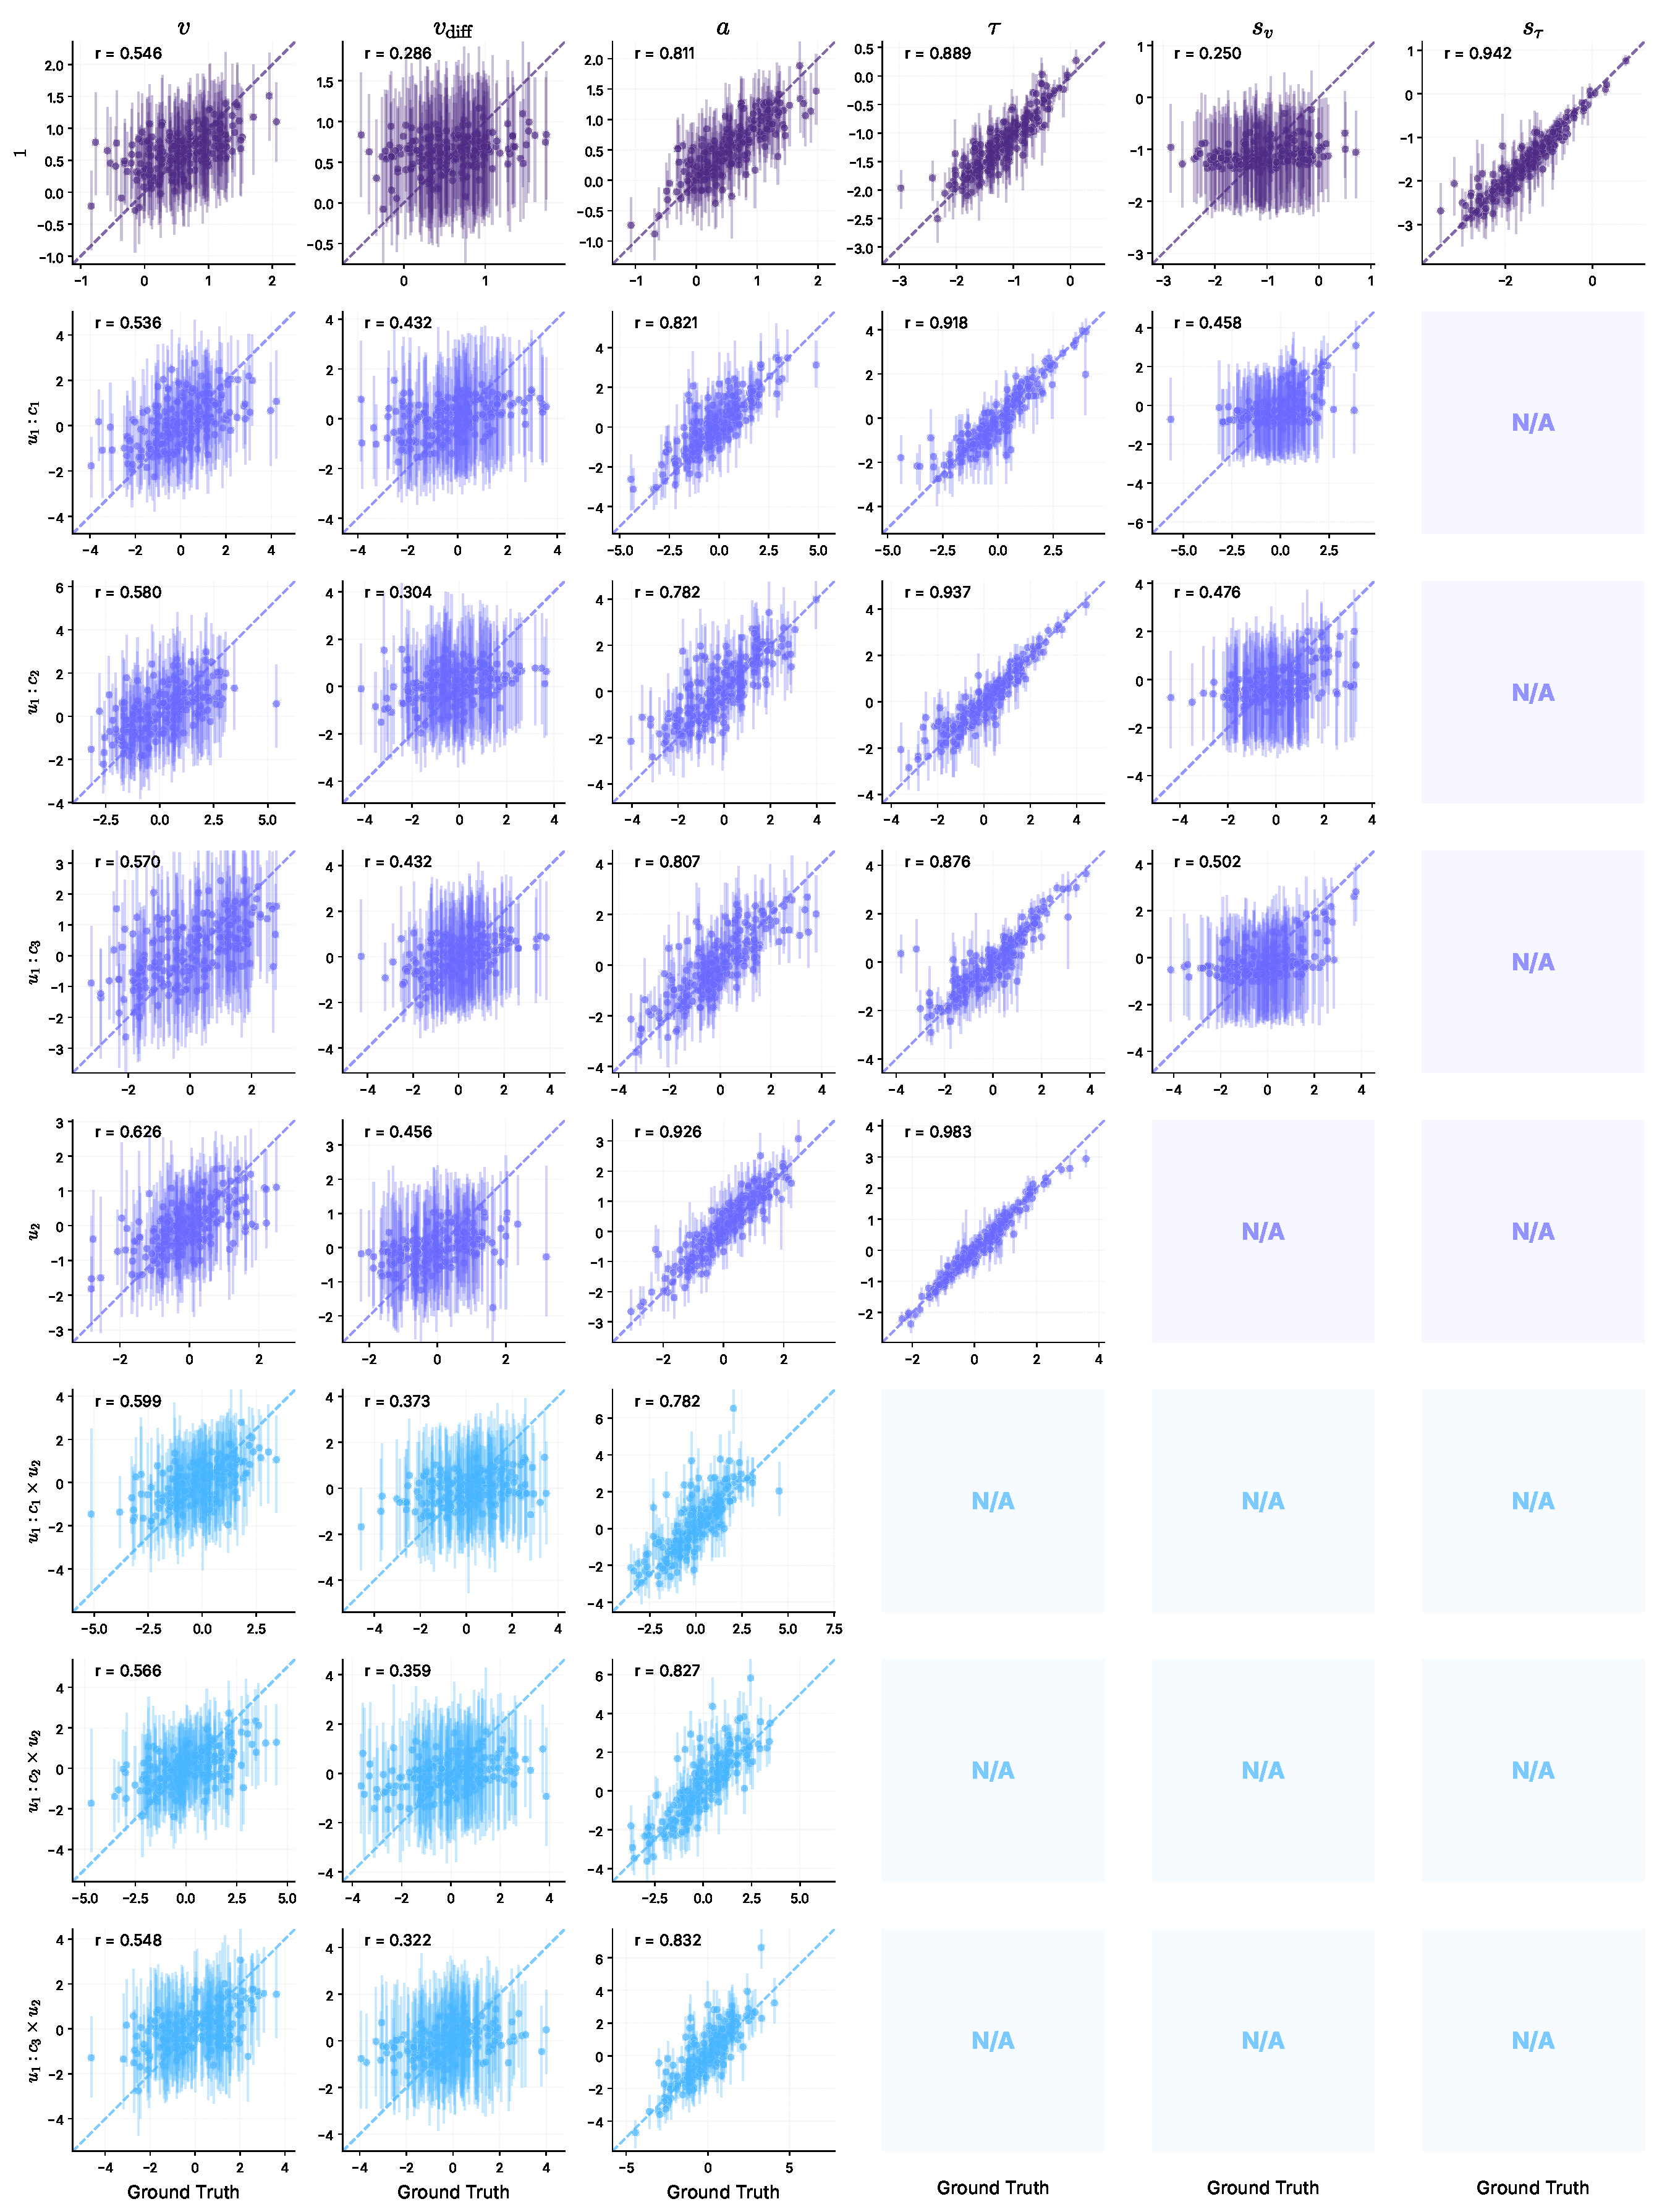
\includegraphics[width=\linewidth,height=0.84\textheight,keepaspectratio]{per_case/rdm/mixed_predictor/recovery.pdf}
  \caption[RDM, mixed-predictor: recovery]{\textbf{RDM, mixed-predictor design --- coefficient
    recovery.} Posterior mean (points) with 95\% credible intervals against the
    data-generating value, one panel per active cell of the coefficient matrix
    $\mathbf{B}$. Columns are intrinsic parameters, rows are design columns
    (intercept, main effects, interactions), labeled by regressor and category;
    the panel axes render this as \texttt{predictor|category}. Inactive cells are
    drawn as grey N/A tiles. Point color encodes the row kind: intercept (purple),
    main effect (blue), interaction (red).}
  \label{fig:e1-rdm-mixed_predictor-rec}
\end{figure}

\begin{figure}[htbp]
  \centering
  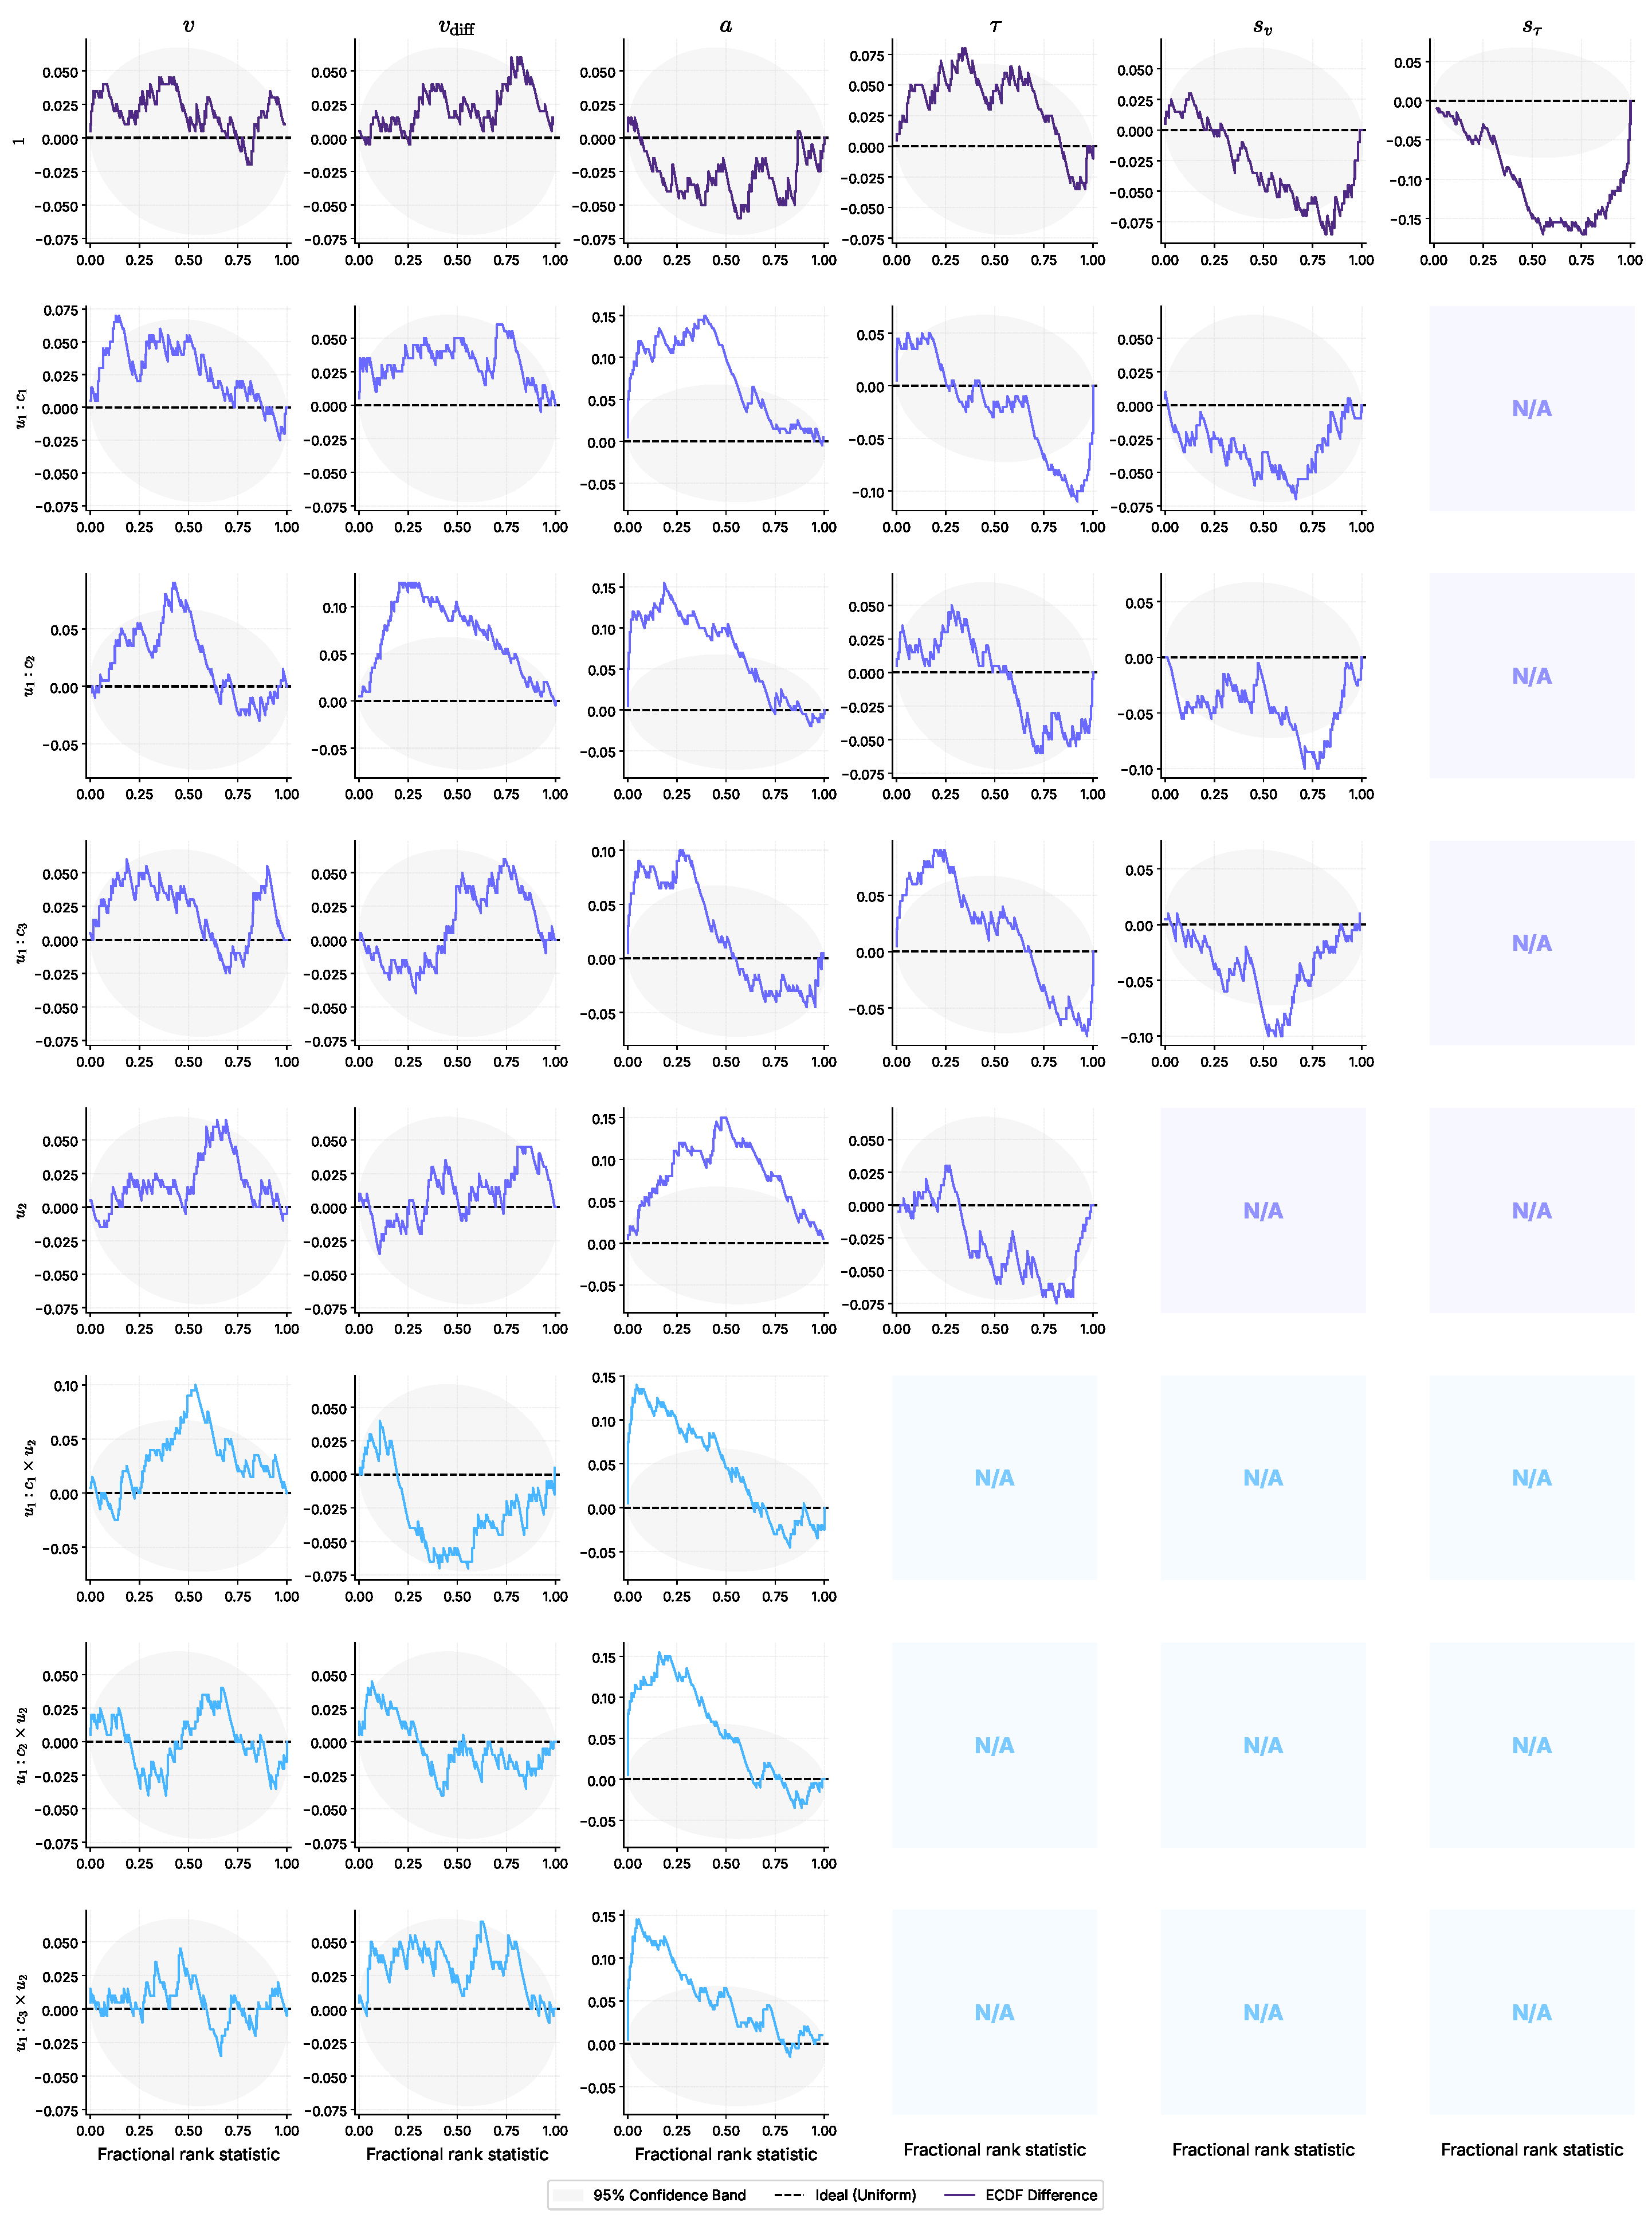
\includegraphics[width=\linewidth,height=0.84\textheight,keepaspectratio]{per_case/rdm/mixed_predictor/ecdf.pdf}
  \caption[RDM, mixed-predictor: ECDF calibration]{\textbf{RDM, mixed-predictor design --- ECDF
    calibration.} Rank-ECDF difference (empirical minus uniform) with simultaneous
    95\% confidence bands, on the same cell layout as the corresponding recovery
    figure (Figure~\ref{fig:e1-rdm-mixed_predictor-rec}). A calibrated posterior stays
    inside the band; excursions above/below indicate bias, and a systematically
    shallow/steep curve indicates over-/under-dispersion.}
  \label{fig:e1-rdm-mixed_predictor-ecdf}
\end{figure}

\FloatBarrier
\clearpage

%-----------------------------------------------------------------------------
\subsection{Circular diffusion model (CDM)}
\label{sec:e1-cdm}
%-----------------------------------------------------------------------------

Intrinsic parameters: drift magnitude $v$, drift angle $v_\theta$, boundary
radius $a$, non-decision time $\tau$, and the dispersions $s_v, s_\tau$.

\begin{figure}[htbp]
  \centering
  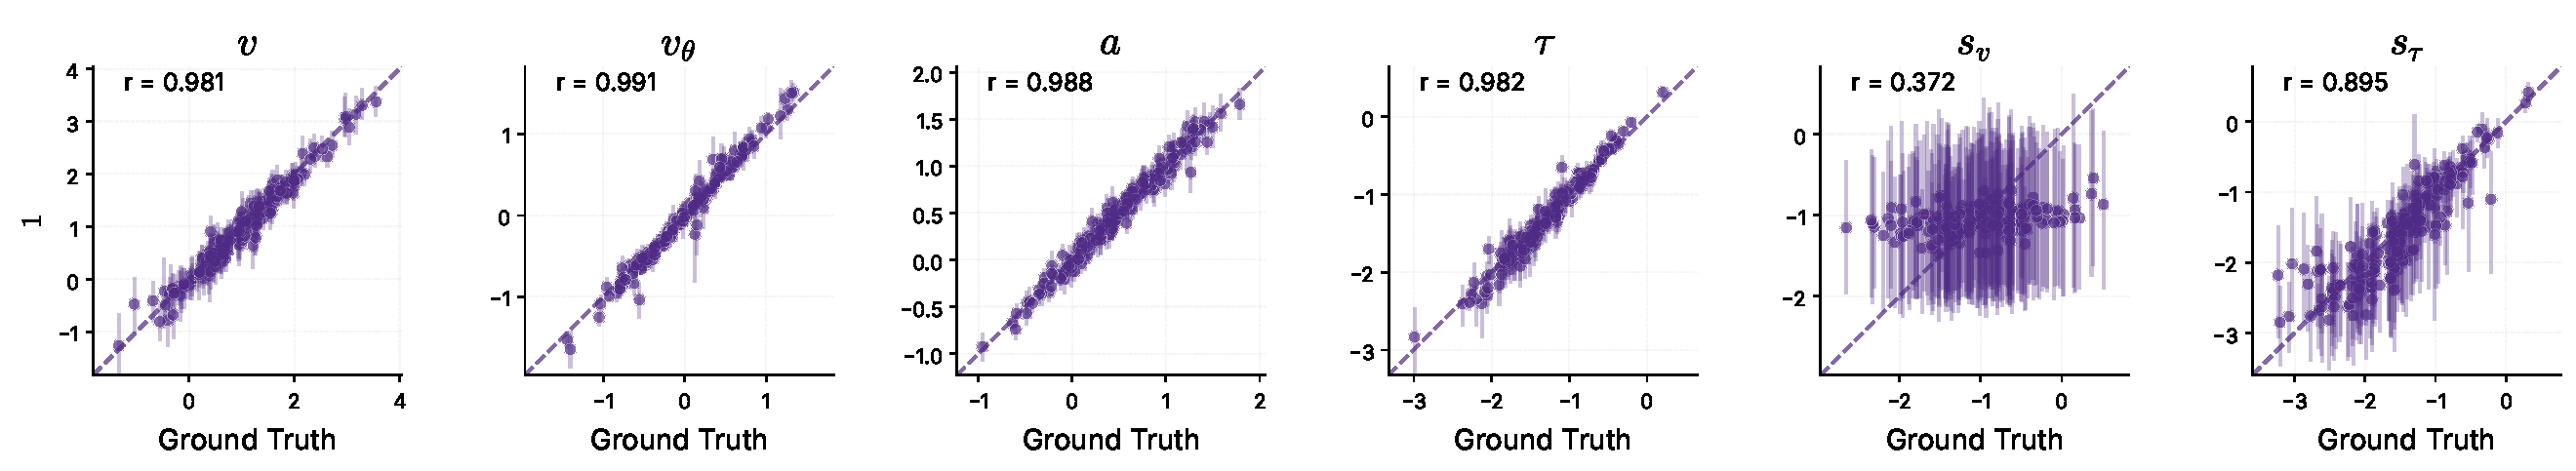
\includegraphics[width=\linewidth,height=0.84\textheight,keepaspectratio]{per_case/cdm/intercept_only/recovery.pdf}
  \caption[CDM, intercept-only: recovery]{\textbf{CDM, intercept-only design --- coefficient
    recovery.} Posterior mean (points) with 95\% credible intervals against the
    data-generating value, one panel per active cell of the coefficient matrix
    $\mathbf{B}$. Columns are intrinsic parameters, rows are design columns
    (intercept, main effects, interactions), labeled by regressor and category;
    the panel axes render this as \texttt{predictor|category}. Inactive cells are
    drawn as grey N/A tiles. Point color encodes the row kind: intercept (purple),
    main effect (blue), interaction (red).}
  \label{fig:e1-cdm-intercept_only-rec}
\end{figure}

\begin{figure}[htbp]
  \centering
  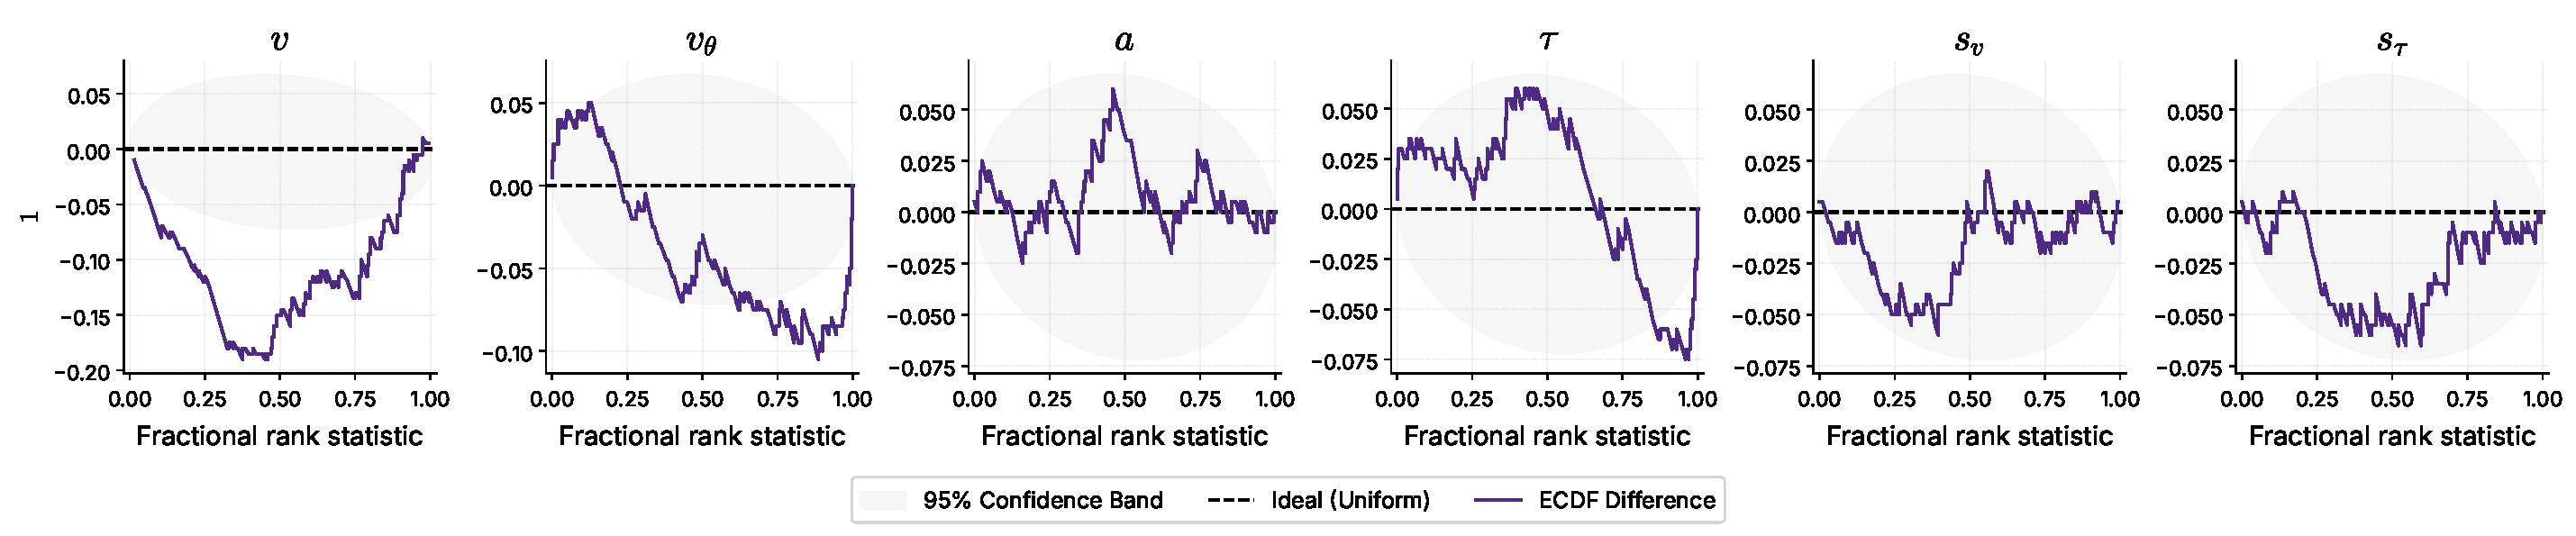
\includegraphics[width=\linewidth,height=0.84\textheight,keepaspectratio]{per_case/cdm/intercept_only/ecdf.pdf}
  \caption[CDM, intercept-only: ECDF calibration]{\textbf{CDM, intercept-only design --- ECDF
    calibration.} Rank-ECDF difference (empirical minus uniform) with simultaneous
    95\% confidence bands, on the same cell layout as the corresponding recovery
    figure (Figure~\ref{fig:e1-cdm-intercept_only-rec}). A calibrated posterior stays
    inside the band; excursions above/below indicate bias, and a systematically
    shallow/steep curve indicates over-/under-dispersion.}
  \label{fig:e1-cdm-intercept_only-ecdf}
\end{figure}

\begin{figure}[htbp]
  \centering
  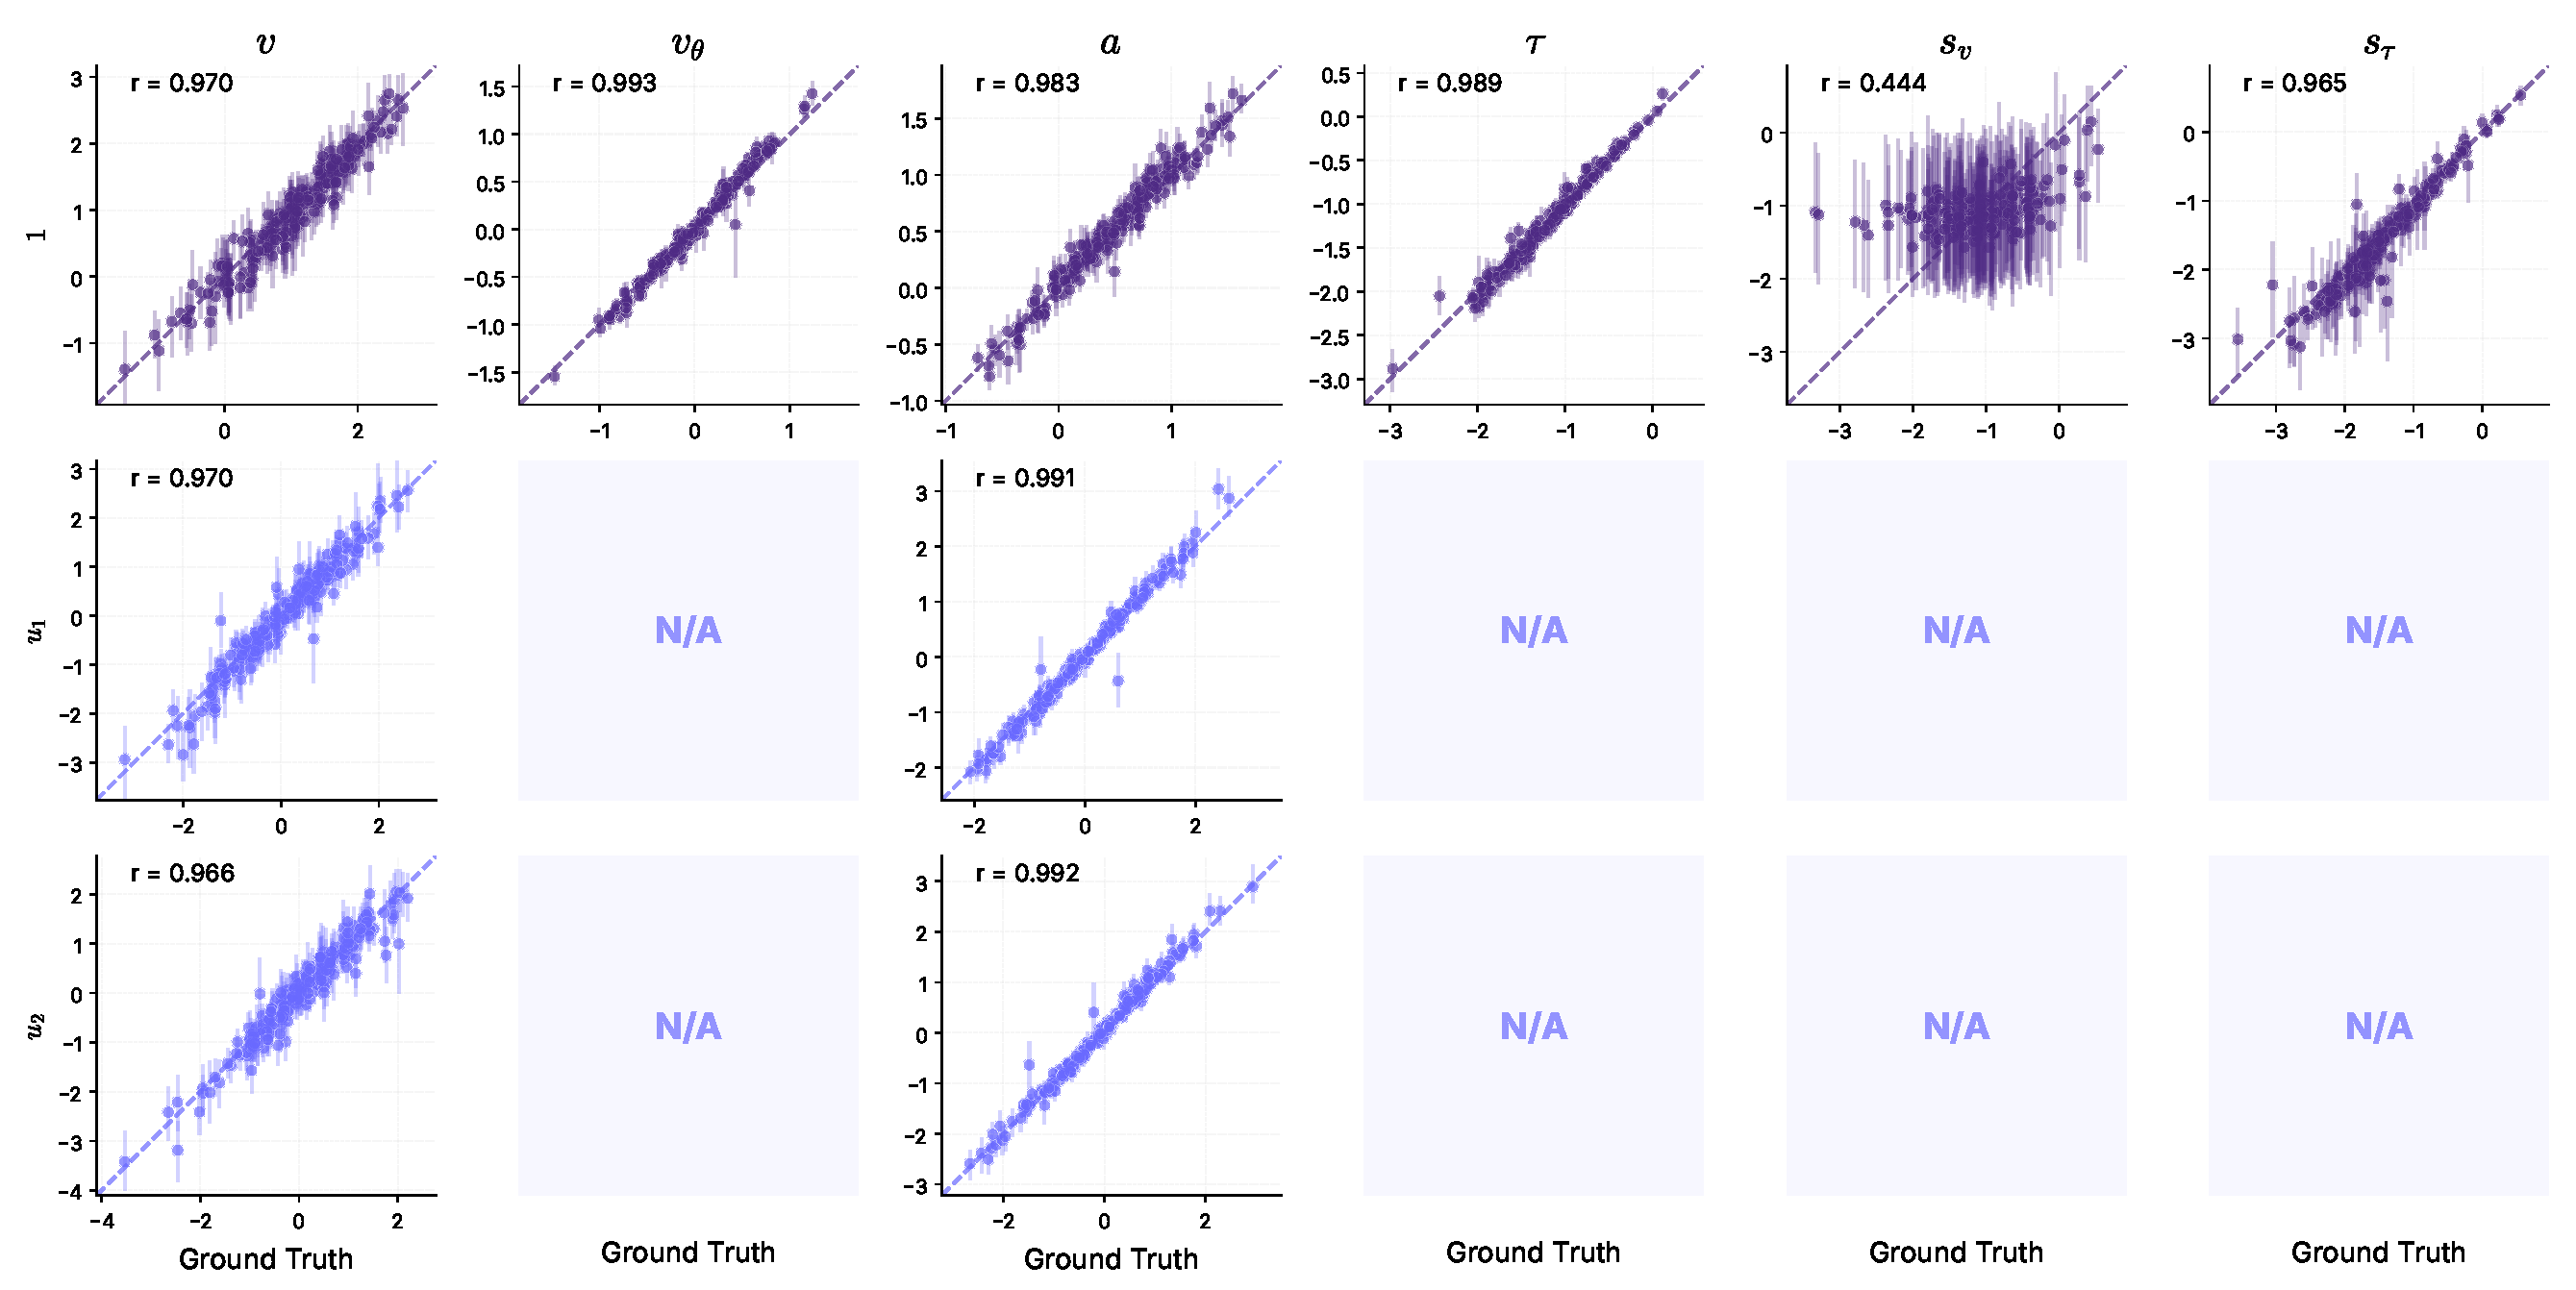
\includegraphics[width=\linewidth,height=0.84\textheight,keepaspectratio]{per_case/cdm/regressed/recovery.pdf}
  \caption[CDM, regressed: recovery]{\textbf{CDM, regressed design --- coefficient
    recovery.} Posterior mean (points) with 95\% credible intervals against the
    data-generating value, one panel per active cell of the coefficient matrix
    $\mathbf{B}$. Columns are intrinsic parameters, rows are design columns
    (intercept, main effects, interactions), labeled by regressor and category;
    the panel axes render this as \texttt{predictor|category}. Inactive cells are
    drawn as grey N/A tiles. Point color encodes the row kind: intercept (purple),
    main effect (blue), interaction (red).}
  \label{fig:e1-cdm-regressed-rec}
\end{figure}

\begin{figure}[htbp]
  \centering
  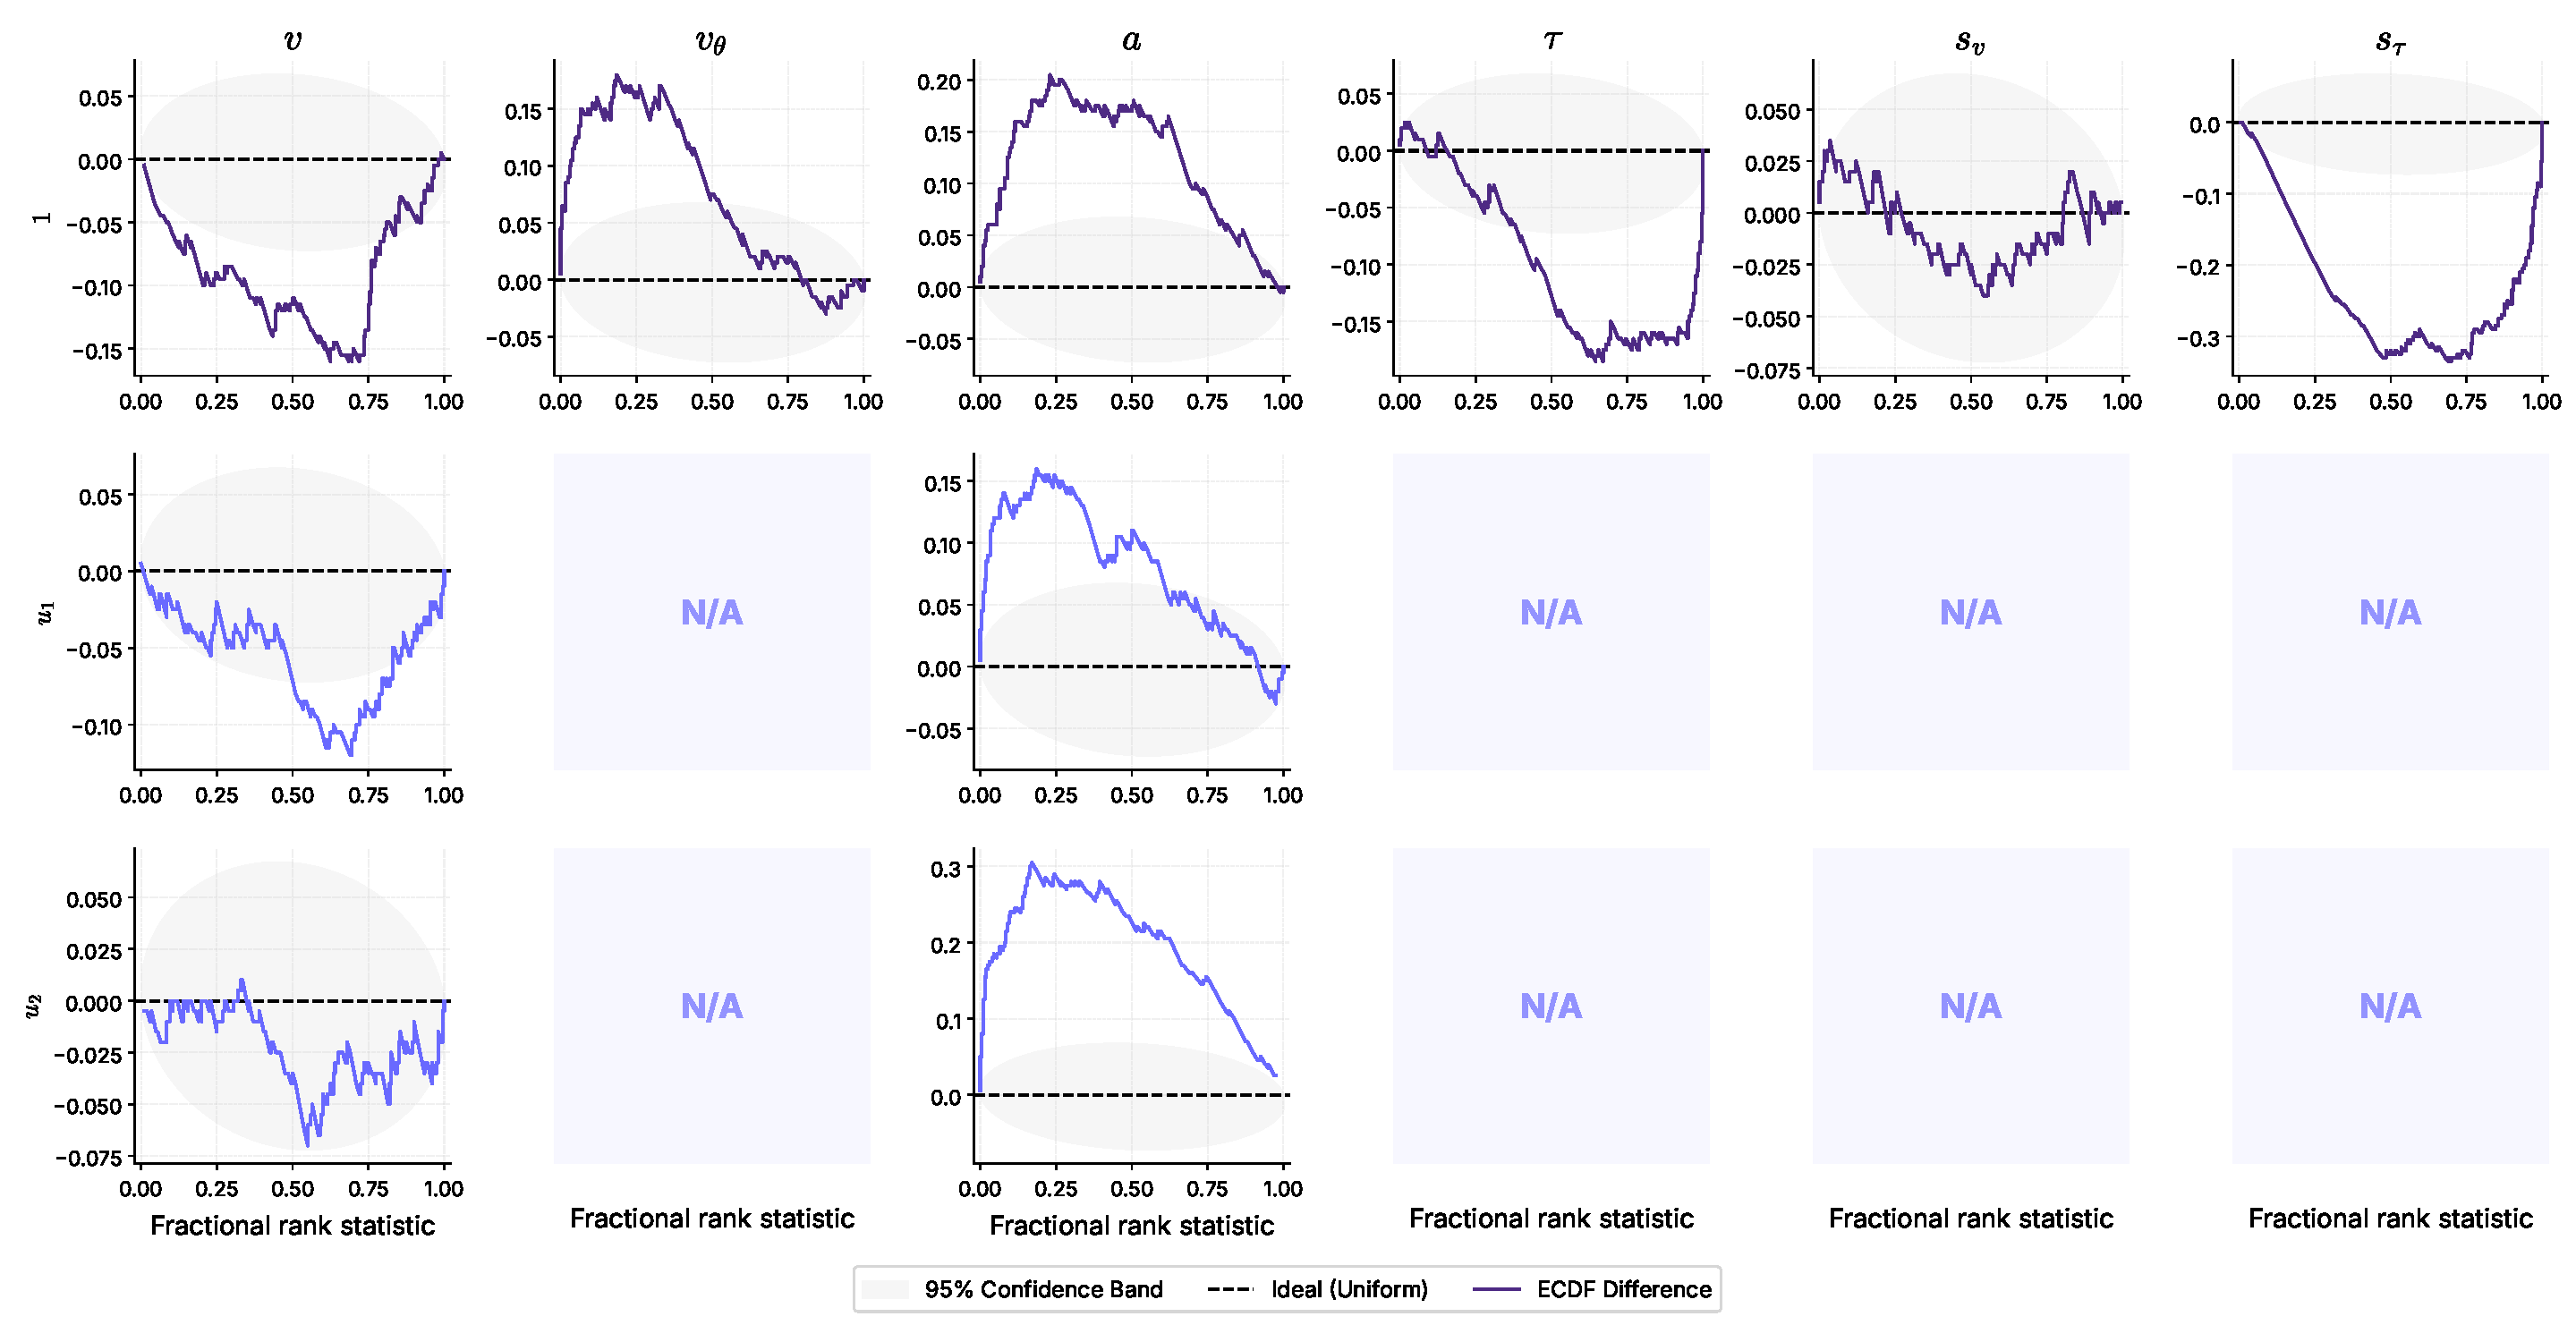
\includegraphics[width=\linewidth,height=0.84\textheight,keepaspectratio]{per_case/cdm/regressed/ecdf.pdf}
  \caption[CDM, regressed: ECDF calibration]{\textbf{CDM, regressed design --- ECDF
    calibration.} Rank-ECDF difference (empirical minus uniform) with simultaneous
    95\% confidence bands, on the same cell layout as the corresponding recovery
    figure (Figure~\ref{fig:e1-cdm-regressed-rec}). A calibrated posterior stays
    inside the band; excursions above/below indicate bias, and a systematically
    shallow/steep curve indicates over-/under-dispersion.}
  \label{fig:e1-cdm-regressed-ecdf}
\end{figure}

\begin{figure}[htbp]
  \centering
  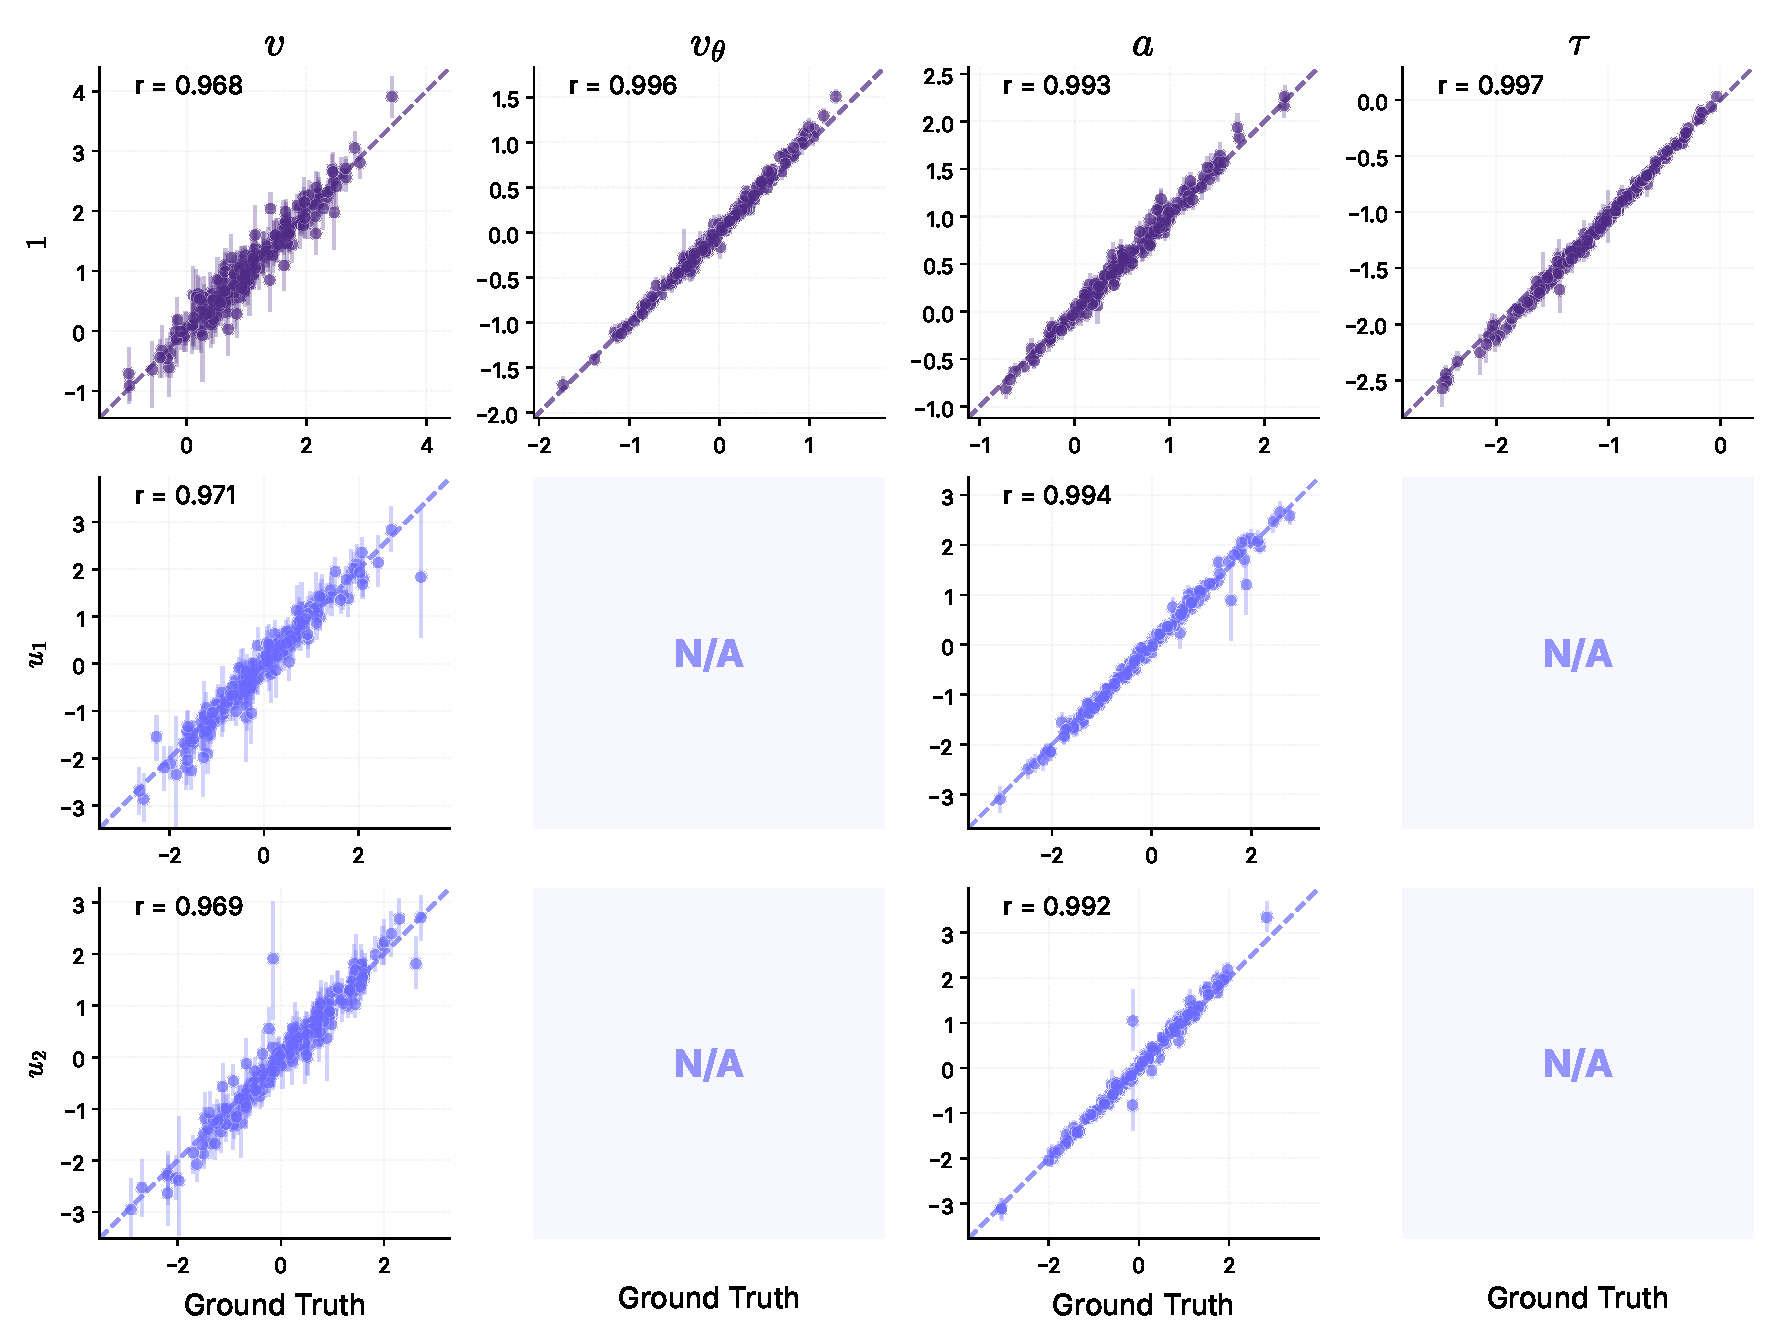
\includegraphics[width=\linewidth,height=0.84\textheight,keepaspectratio]{per_case/cdm/fixed_regressed/recovery.pdf}
  \caption[CDM, fixed-regressed: recovery]{\textbf{CDM, fixed-regressed design --- coefficient
    recovery.} Posterior mean (points) with 95\% credible intervals against the
    data-generating value, one panel per active cell of the coefficient matrix
    $\mathbf{B}$. Columns are intrinsic parameters, rows are design columns
    (intercept, main effects, interactions), labeled by regressor and category;
    the panel axes render this as \texttt{predictor|category}. Inactive cells are
    drawn as grey N/A tiles. Point color encodes the row kind: intercept (purple),
    main effect (blue), interaction (red).}
  \label{fig:e1-cdm-fixed_regressed-rec}
\end{figure}

\begin{figure}[htbp]
  \centering
  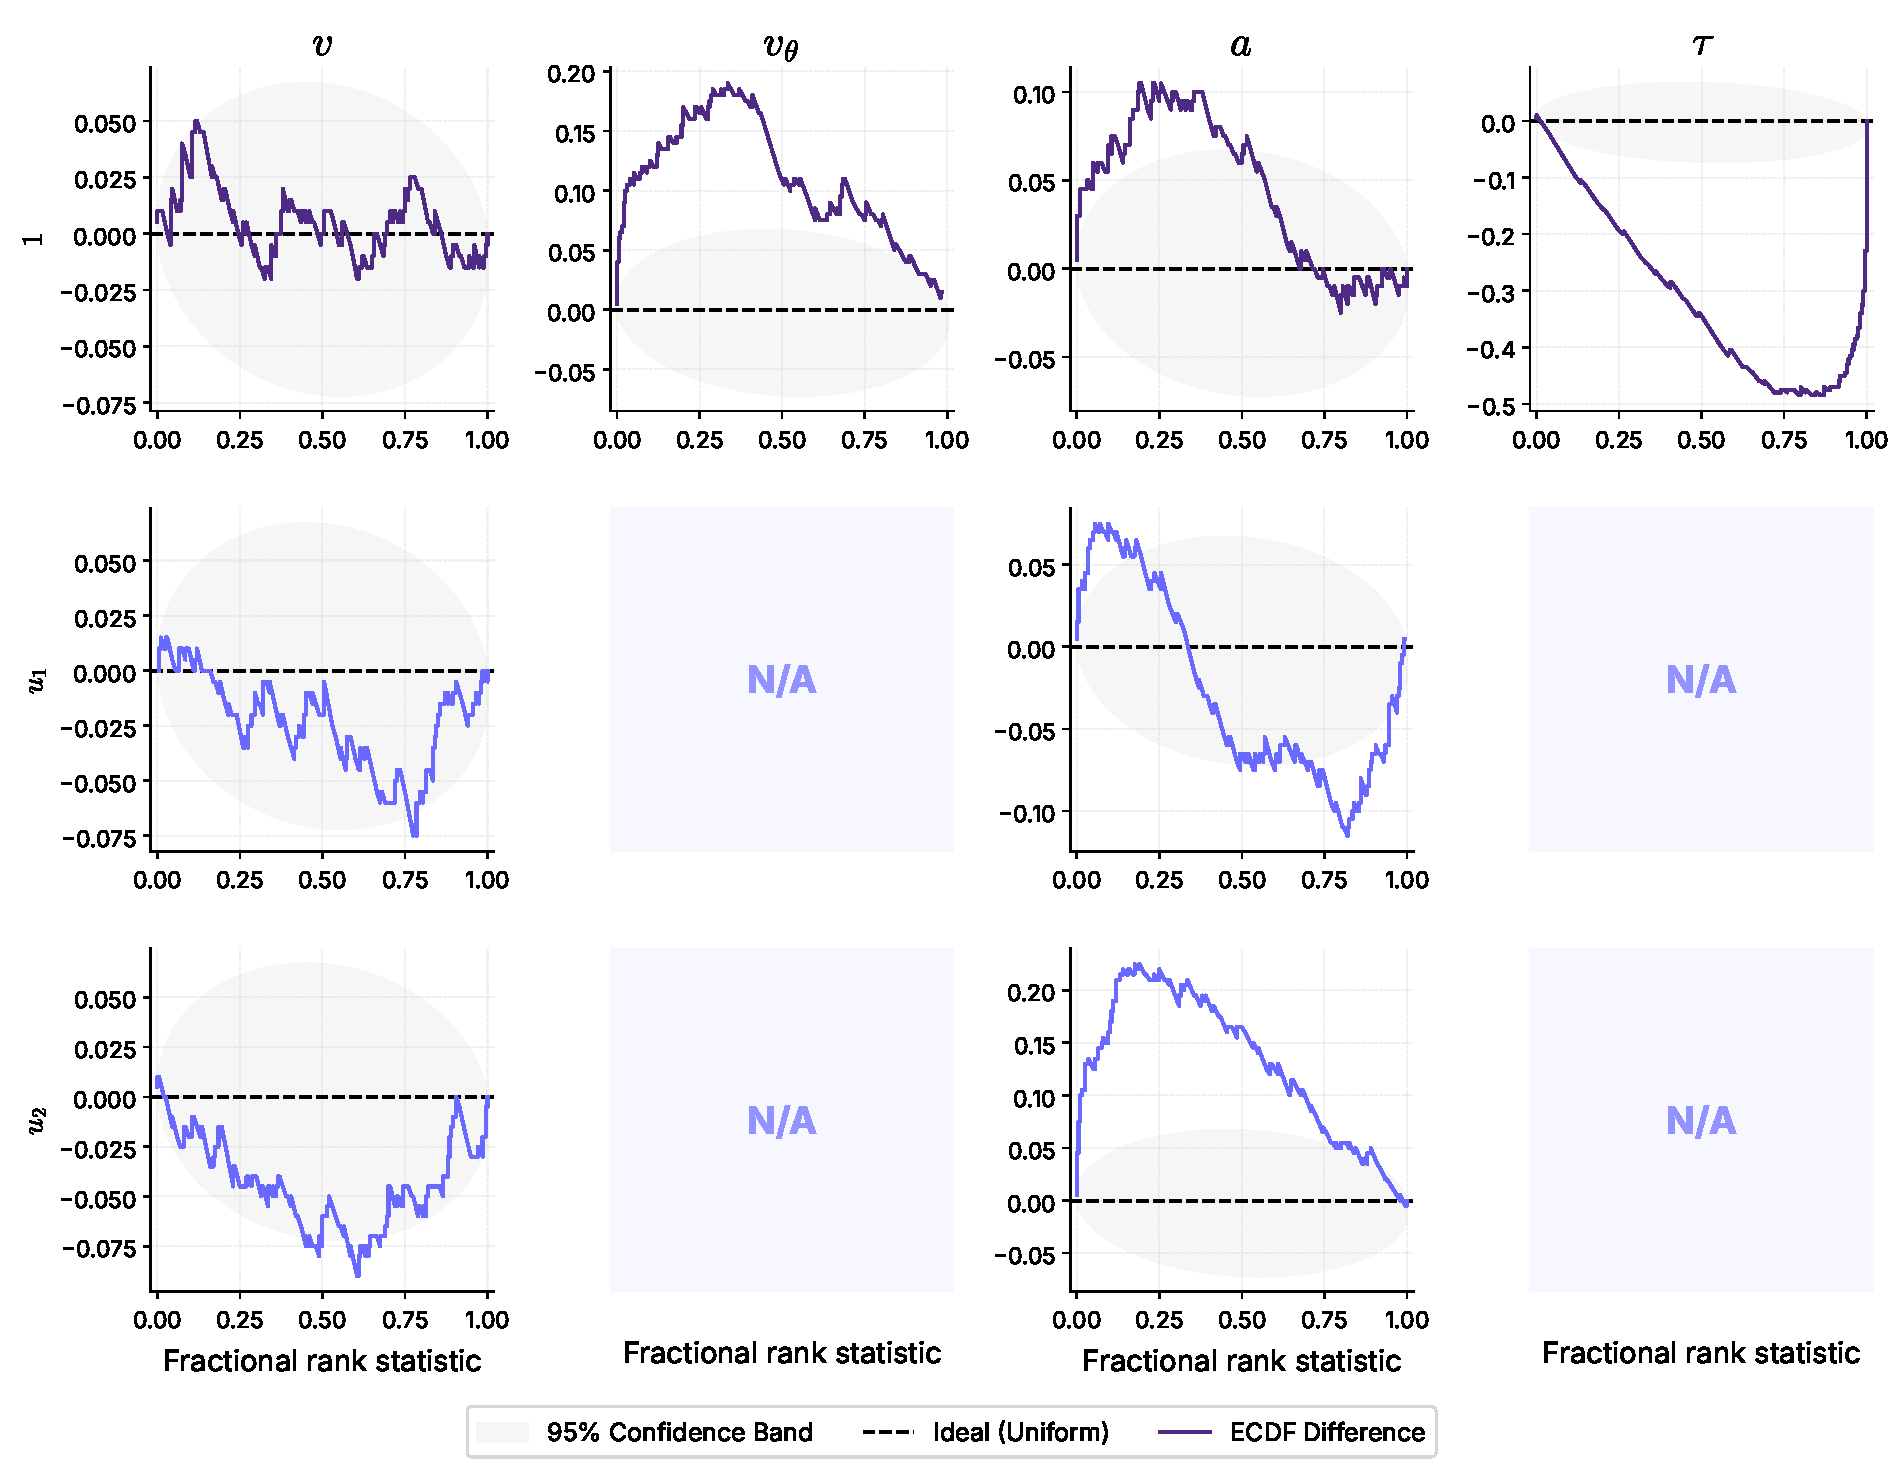
\includegraphics[width=\linewidth,height=0.84\textheight,keepaspectratio]{per_case/cdm/fixed_regressed/ecdf.pdf}
  \caption[CDM, fixed-regressed: ECDF calibration]{\textbf{CDM, fixed-regressed design --- ECDF
    calibration.} Rank-ECDF difference (empirical minus uniform) with simultaneous
    95\% confidence bands, on the same cell layout as the corresponding recovery
    figure (Figure~\ref{fig:e1-cdm-fixed_regressed-rec}). A calibrated posterior stays
    inside the band; excursions above/below indicate bias, and a systematically
    shallow/steep curve indicates over-/under-dispersion.}
  \label{fig:e1-cdm-fixed_regressed-ecdf}
\end{figure}

\begin{figure}[htbp]
  \centering
  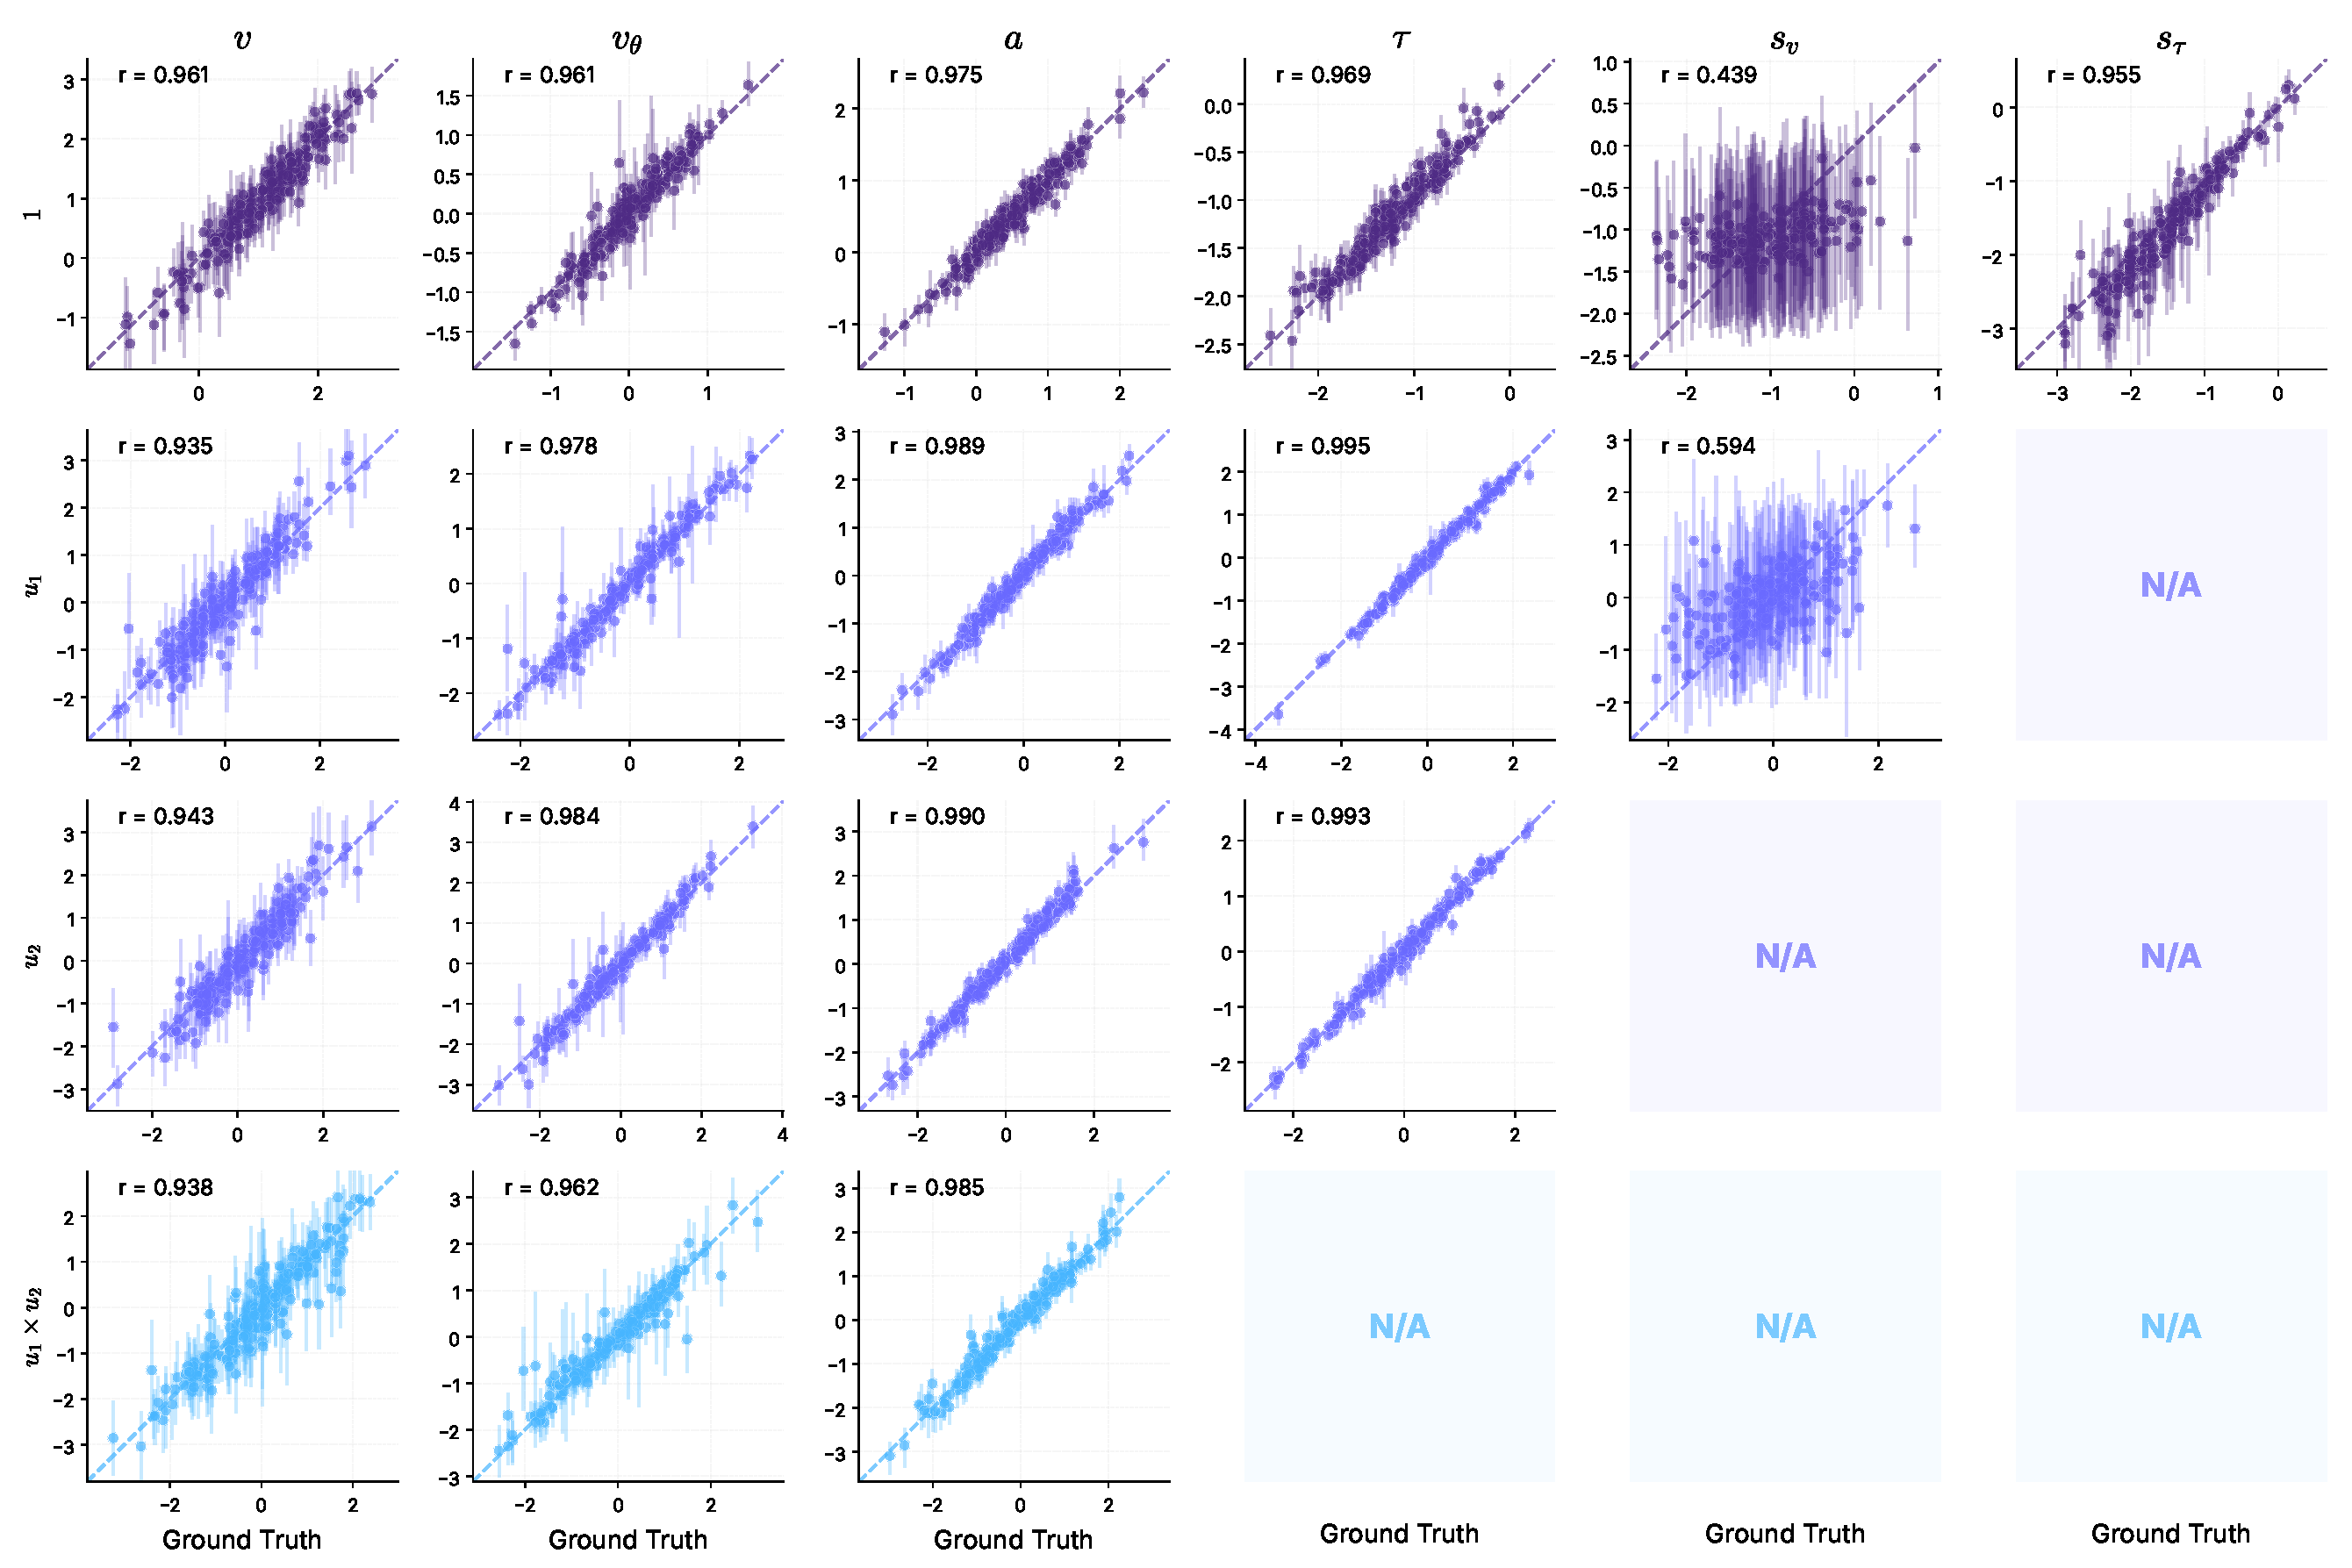
\includegraphics[width=\linewidth,height=0.84\textheight,keepaspectratio]{per_case/cdm/interaction/recovery.pdf}
  \caption[CDM, interaction: recovery]{\textbf{CDM, interaction design --- coefficient
    recovery.} Posterior mean (points) with 95\% credible intervals against the
    data-generating value, one panel per active cell of the coefficient matrix
    $\mathbf{B}$. Columns are intrinsic parameters, rows are design columns
    (intercept, main effects, interactions), labeled by regressor and category;
    the panel axes render this as \texttt{predictor|category}. Inactive cells are
    drawn as grey N/A tiles. Point color encodes the row kind: intercept (purple),
    main effect (blue), interaction (red).}
  \label{fig:e1-cdm-interaction-rec}
\end{figure}

\begin{figure}[htbp]
  \centering
  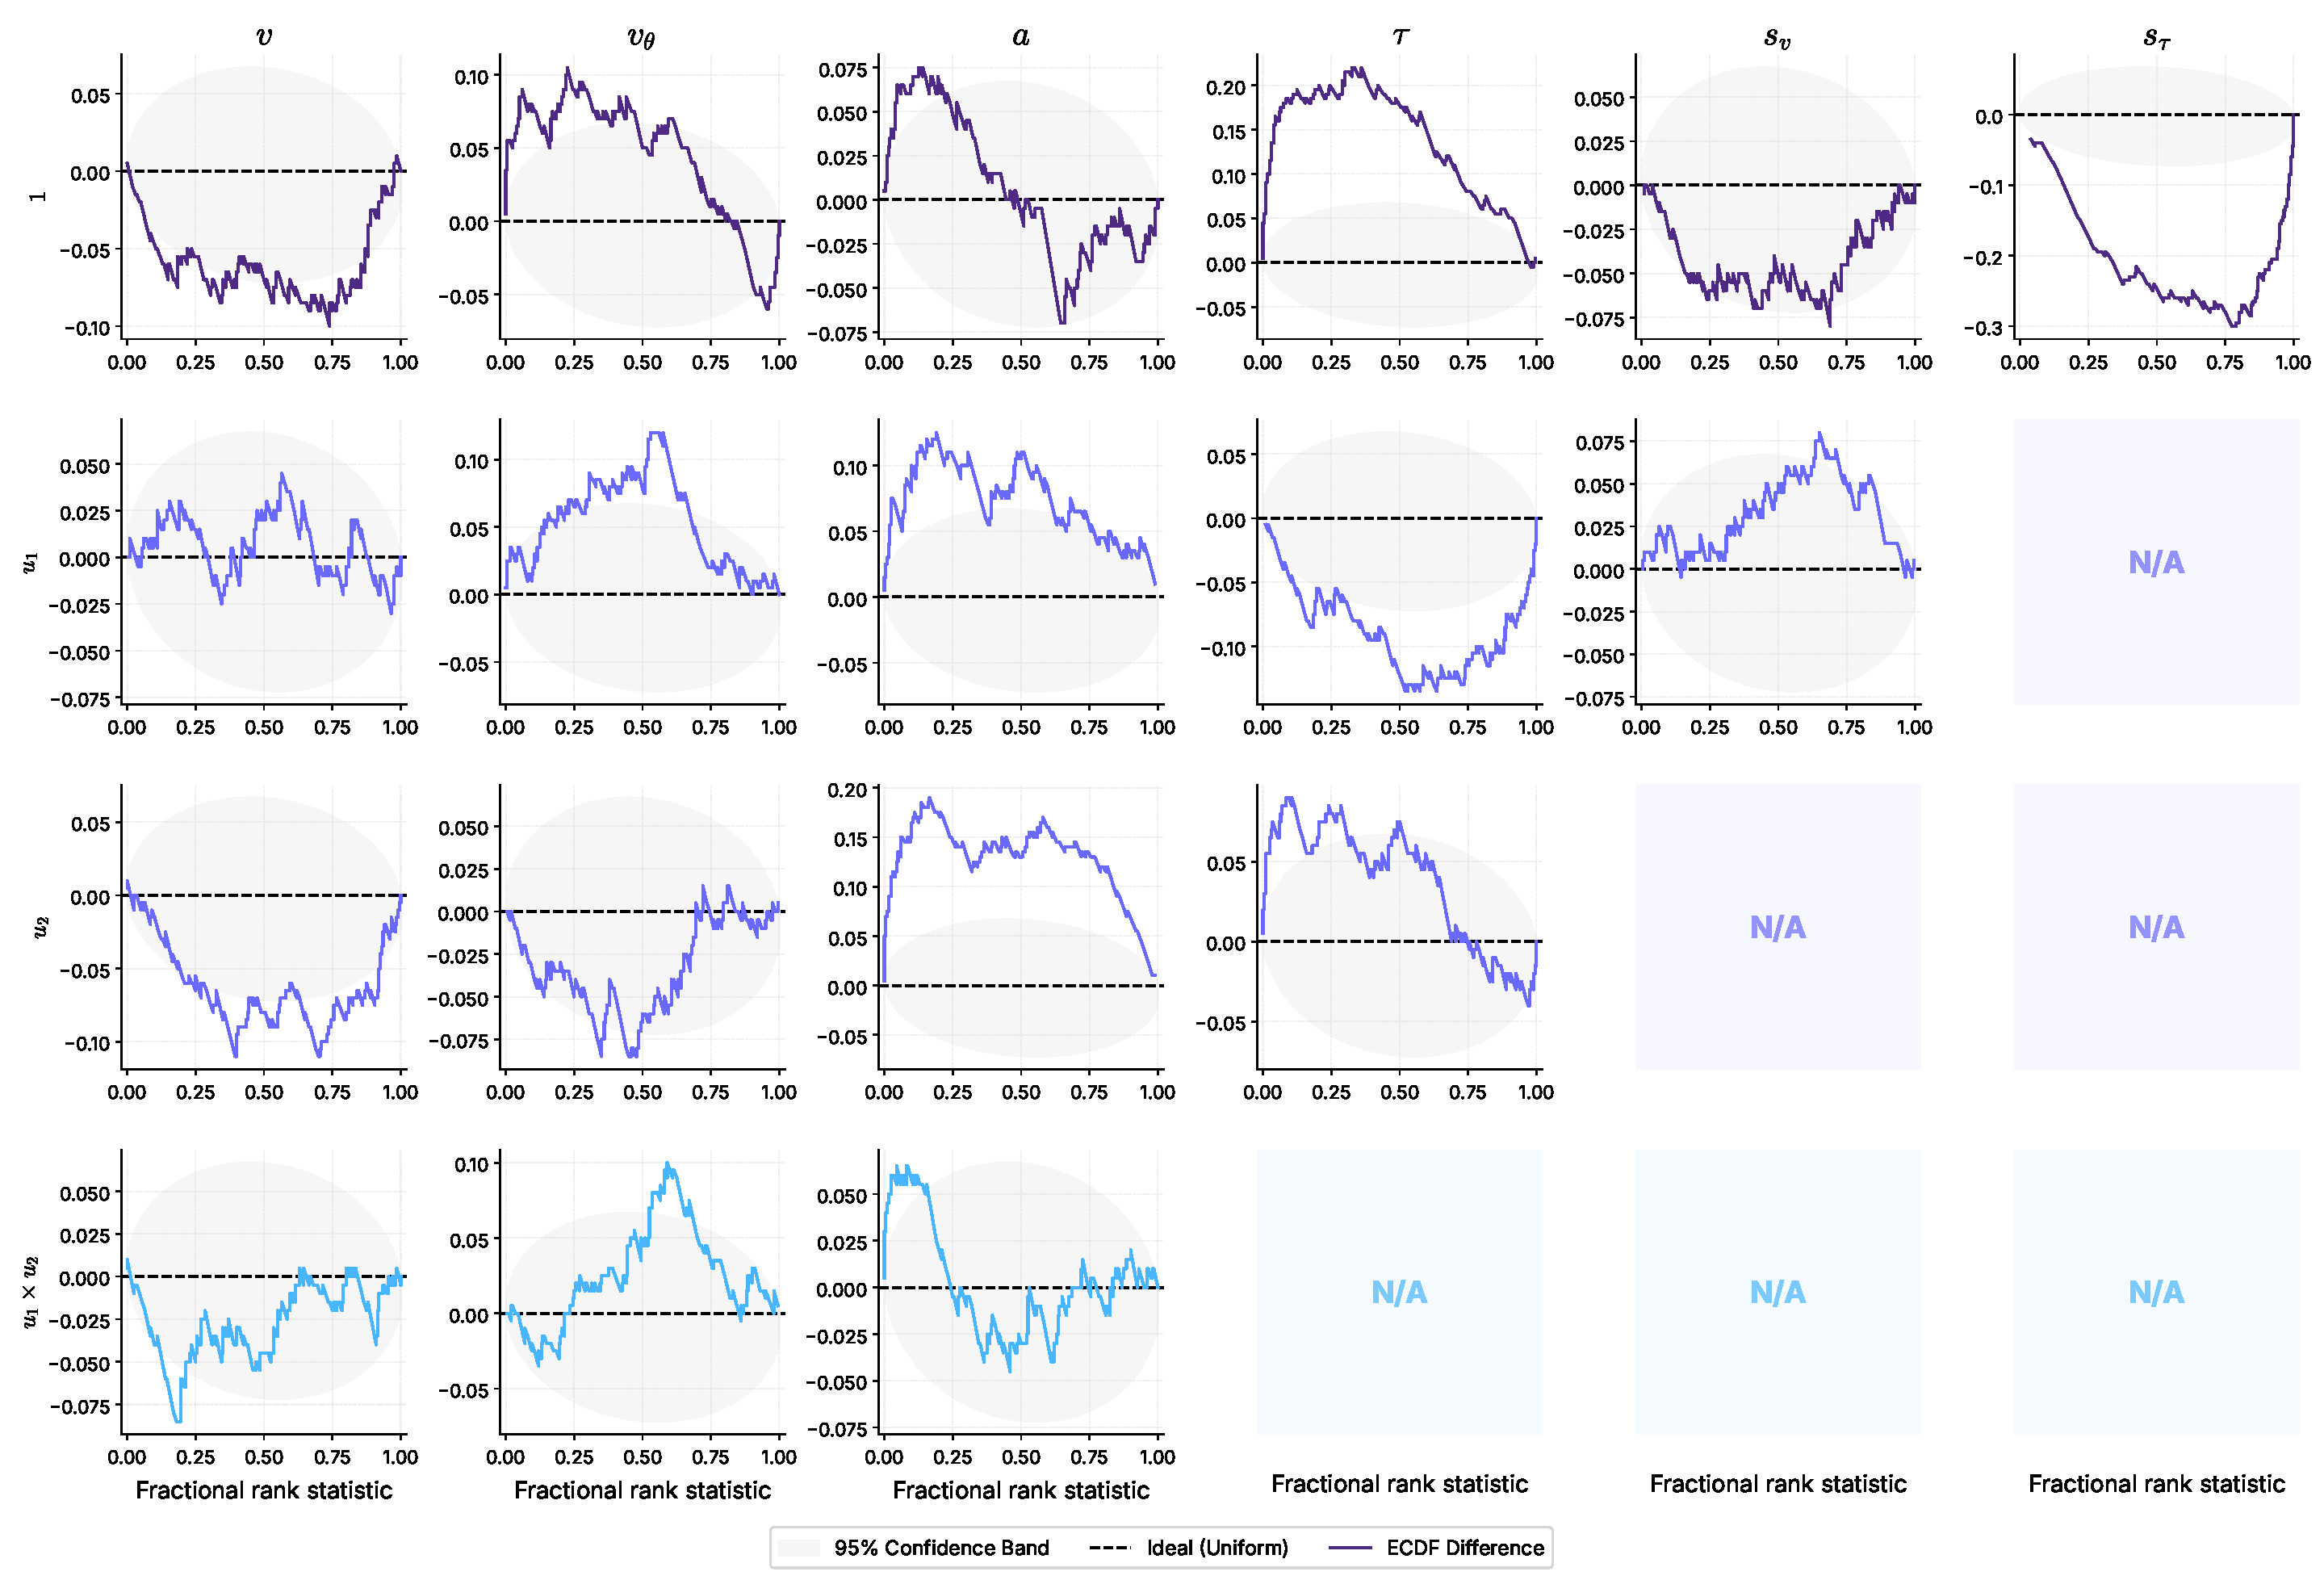
\includegraphics[width=\linewidth,height=0.84\textheight,keepaspectratio]{per_case/cdm/interaction/ecdf.pdf}
  \caption[CDM, interaction: ECDF calibration]{\textbf{CDM, interaction design --- ECDF
    calibration.} Rank-ECDF difference (empirical minus uniform) with simultaneous
    95\% confidence bands, on the same cell layout as the corresponding recovery
    figure (Figure~\ref{fig:e1-cdm-interaction-rec}). A calibrated posterior stays
    inside the band; excursions above/below indicate bias, and a systematically
    shallow/steep curve indicates over-/under-dispersion.}
  \label{fig:e1-cdm-interaction-ecdf}
\end{figure}

\begin{figure}[htbp]
  \centering
  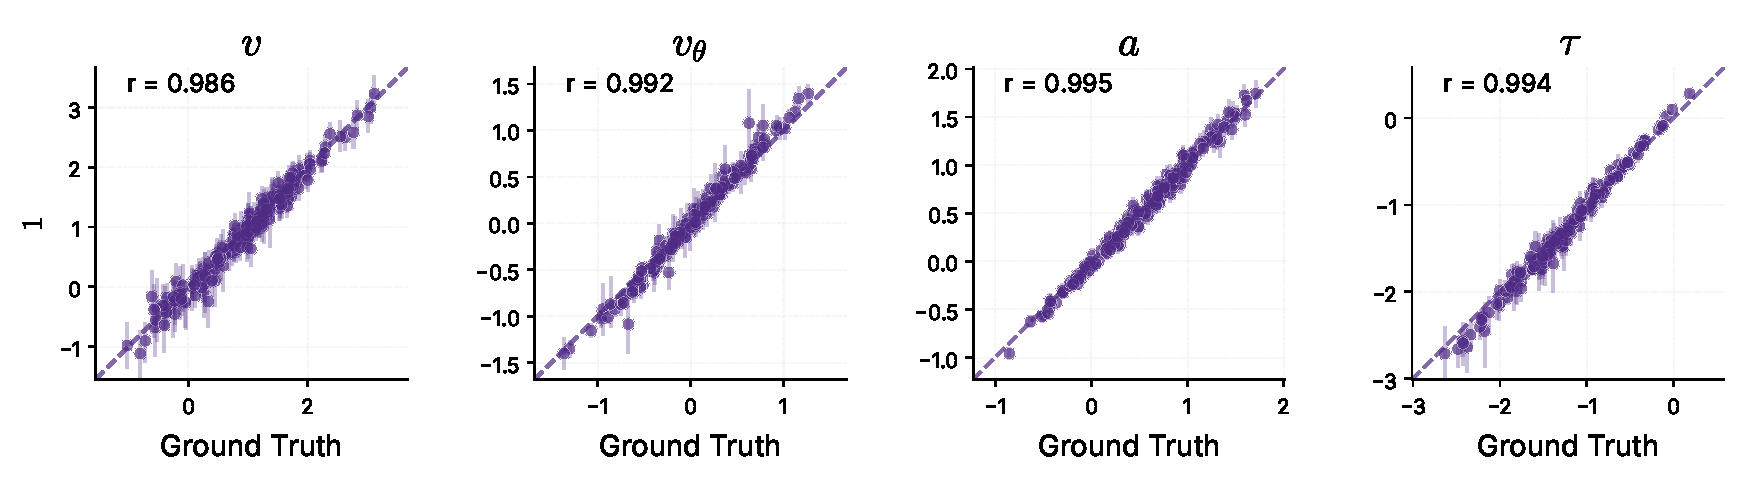
\includegraphics[width=\linewidth,height=0.84\textheight,keepaspectratio]{per_case/cdm/fixed/recovery.pdf}
  \caption[CDM, fixed: recovery]{\textbf{CDM, fixed design --- coefficient
    recovery.} Posterior mean (points) with 95\% credible intervals against the
    data-generating value, one panel per active cell of the coefficient matrix
    $\mathbf{B}$. Columns are intrinsic parameters, rows are design columns
    (intercept, main effects, interactions), labeled by regressor and category;
    the panel axes render this as \texttt{predictor|category}. Inactive cells are
    drawn as grey N/A tiles. Point color encodes the row kind: intercept (purple),
    main effect (blue), interaction (red).}
  \label{fig:e1-cdm-fixed-rec}
\end{figure}

\begin{figure}[htbp]
  \centering
  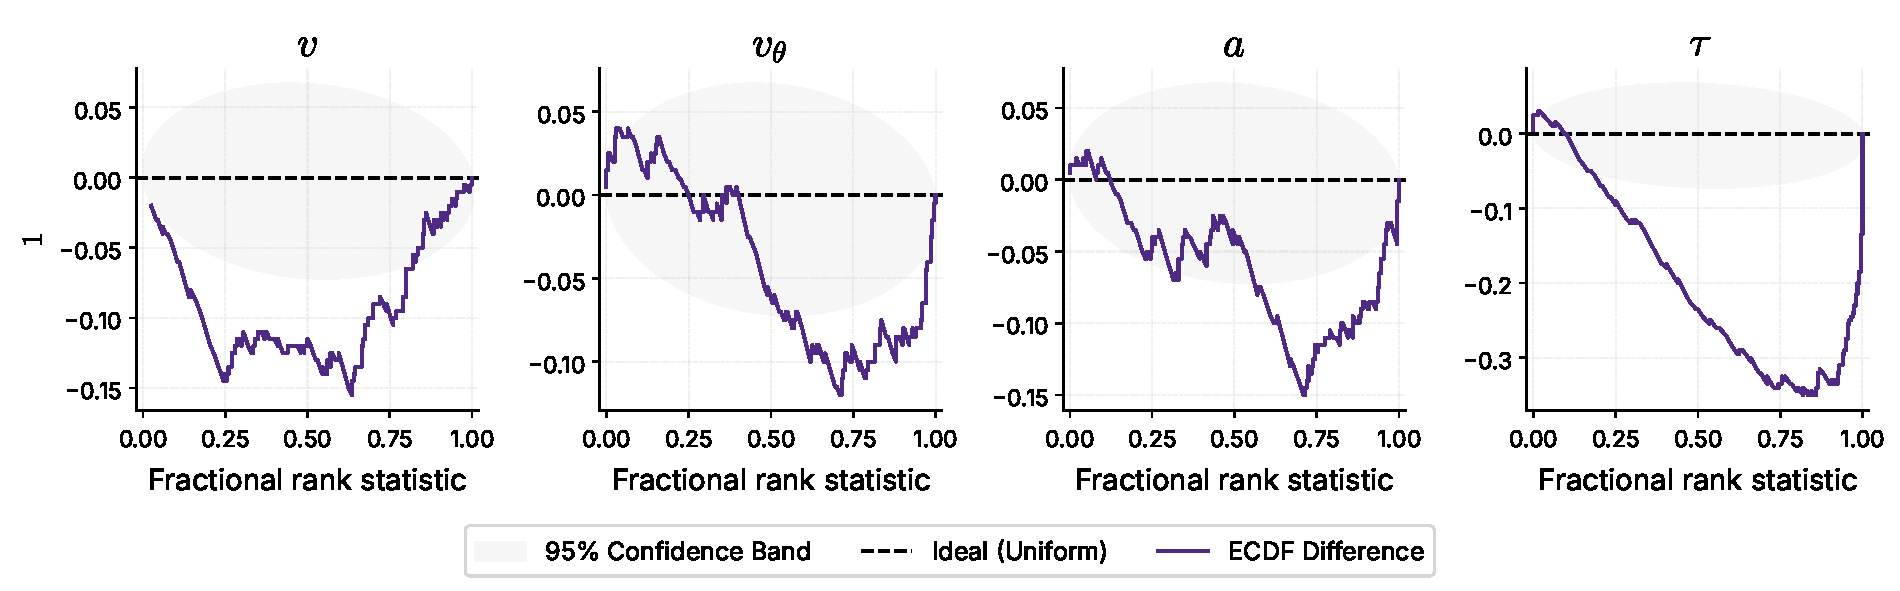
\includegraphics[width=\linewidth,height=0.84\textheight,keepaspectratio]{per_case/cdm/fixed/ecdf.pdf}
  \caption[CDM, fixed: ECDF calibration]{\textbf{CDM, fixed design --- ECDF
    calibration.} Rank-ECDF difference (empirical minus uniform) with simultaneous
    95\% confidence bands, on the same cell layout as the corresponding recovery
    figure (Figure~\ref{fig:e1-cdm-fixed-rec}). A calibrated posterior stays
    inside the band; excursions above/below indicate bias, and a systematically
    shallow/steep curve indicates over-/under-dispersion.}
  \label{fig:e1-cdm-fixed-ecdf}
\end{figure}

\begin{figure}[htbp]
  \centering
  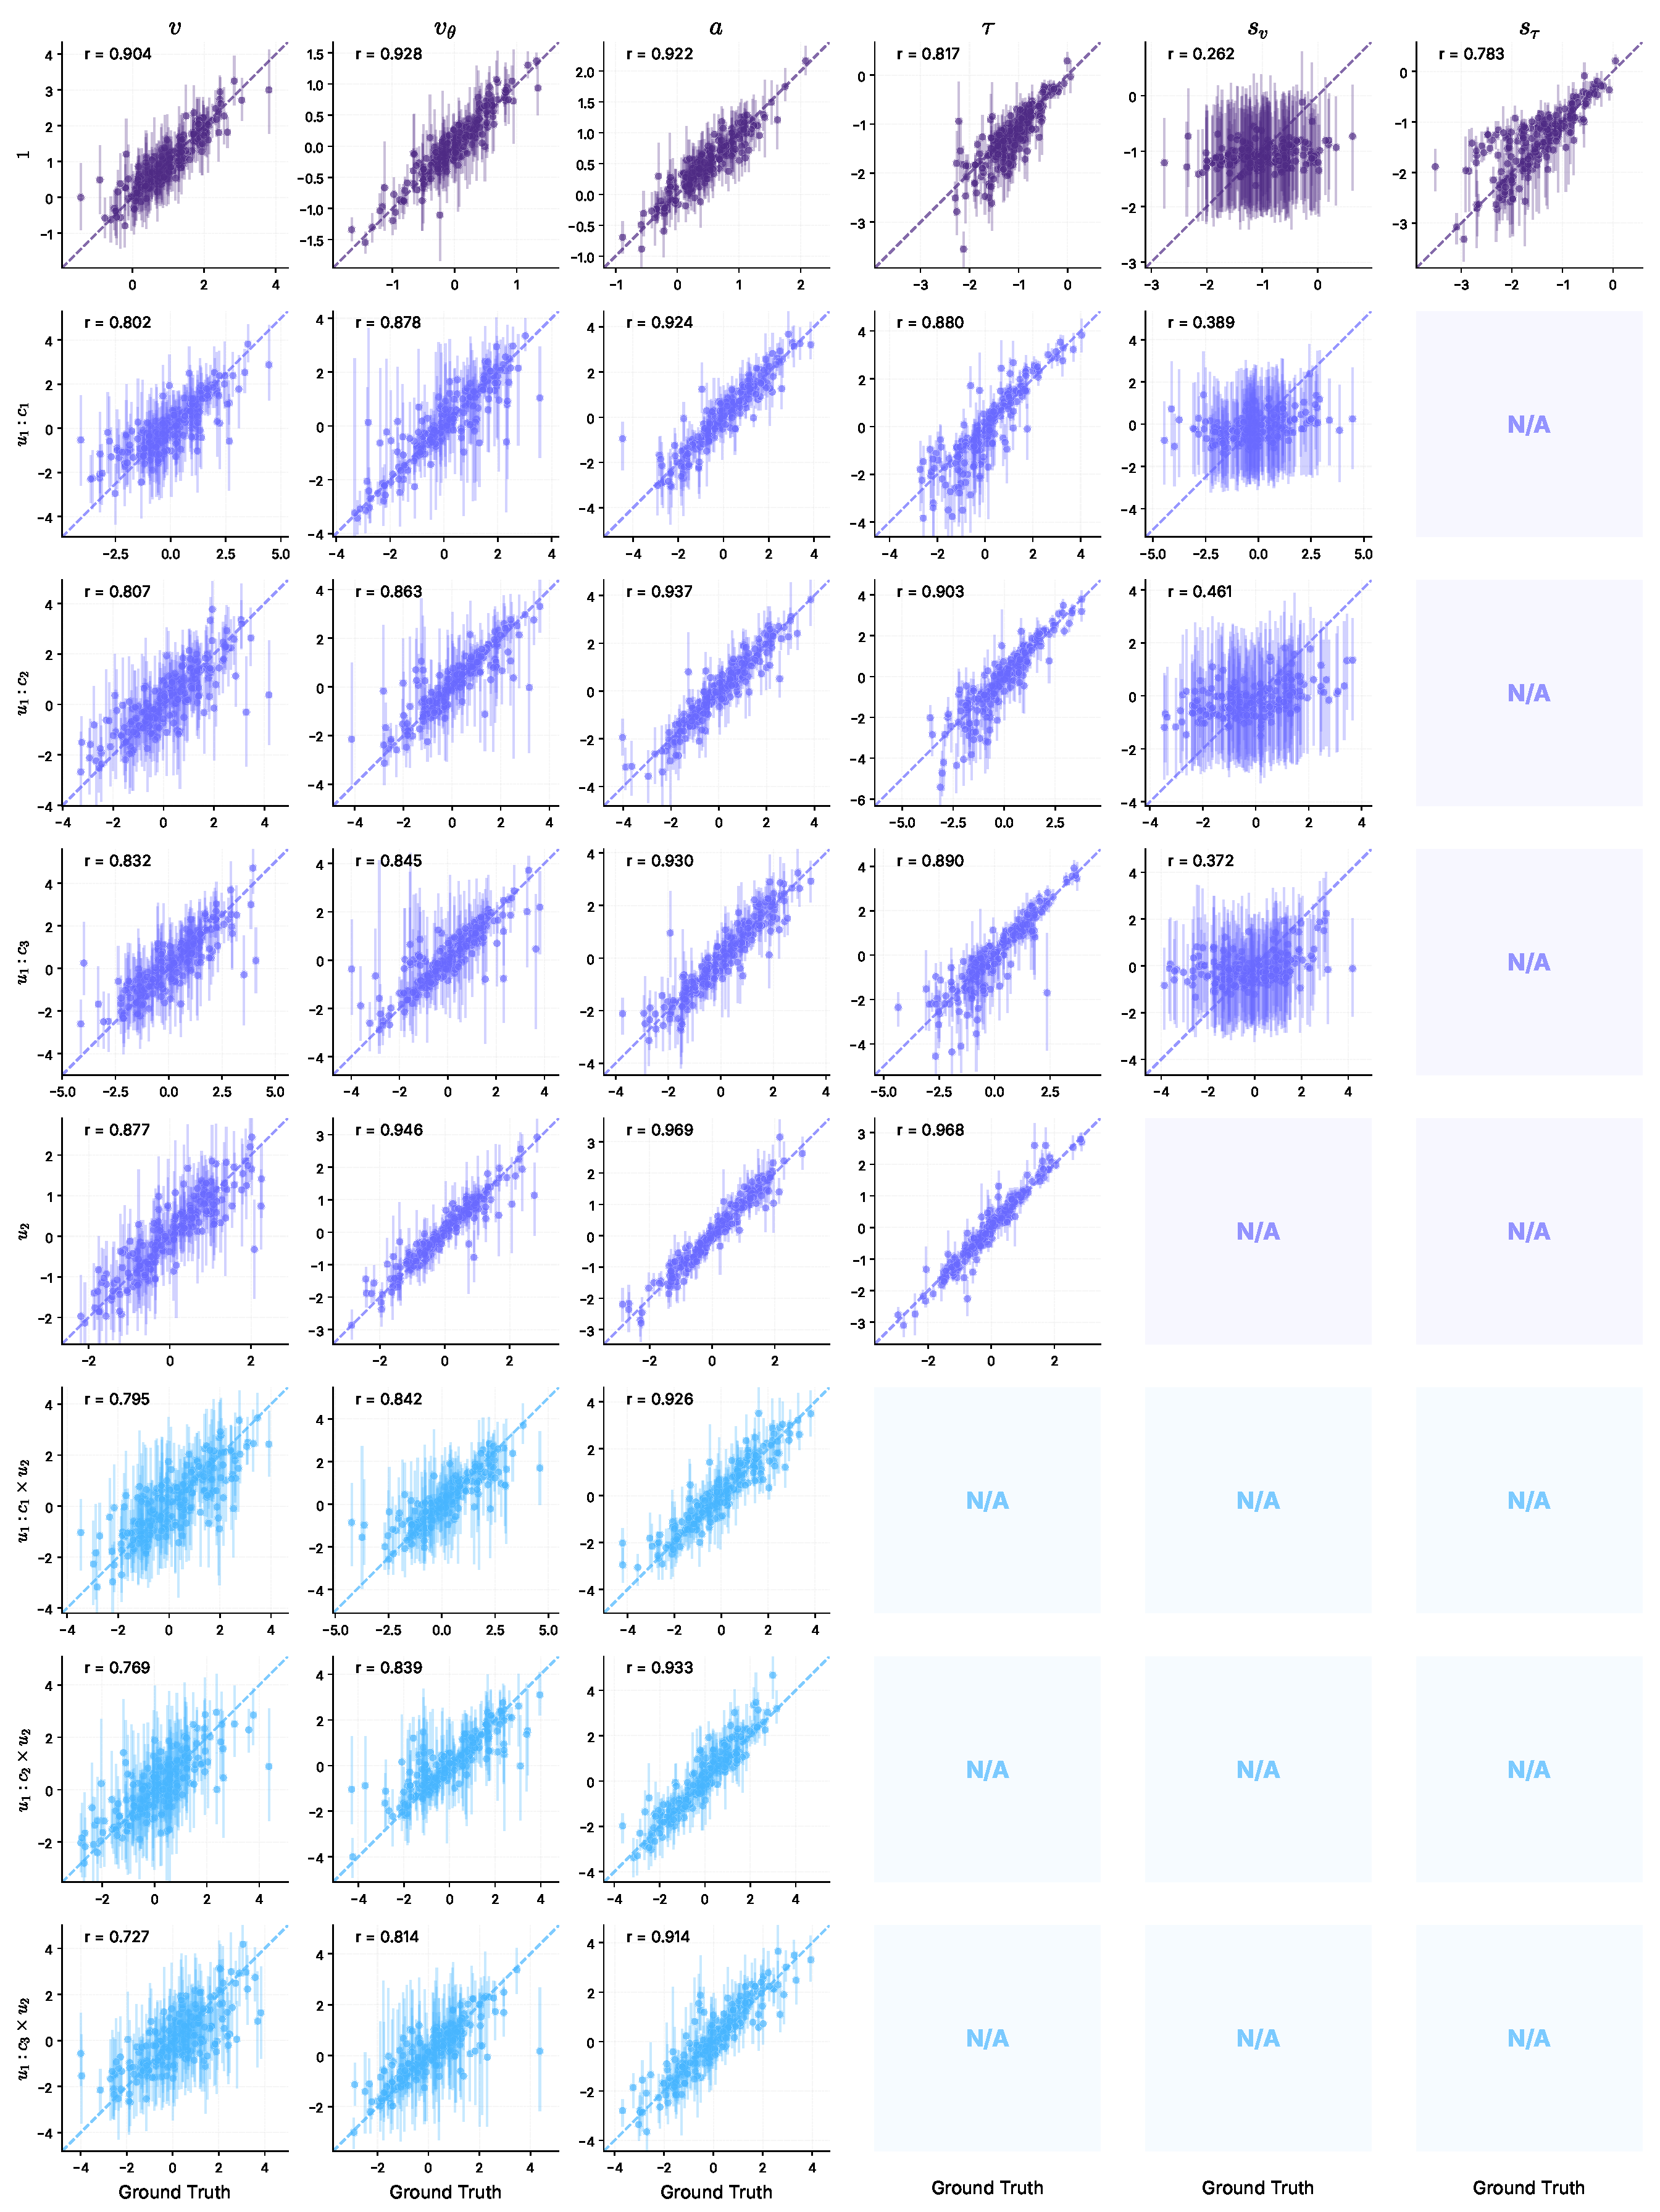
\includegraphics[width=\linewidth,height=0.84\textheight,keepaspectratio]{per_case/cdm/mixed_predictor/recovery.pdf}
  \caption[CDM, mixed-predictor: recovery]{\textbf{CDM, mixed-predictor design --- coefficient
    recovery.} Posterior mean (points) with 95\% credible intervals against the
    data-generating value, one panel per active cell of the coefficient matrix
    $\mathbf{B}$. Columns are intrinsic parameters, rows are design columns
    (intercept, main effects, interactions), labeled by regressor and category;
    the panel axes render this as \texttt{predictor|category}. Inactive cells are
    drawn as grey N/A tiles. Point color encodes the row kind: intercept (purple),
    main effect (blue), interaction (red).}
  \label{fig:e1-cdm-mixed_predictor-rec}
\end{figure}

\begin{figure}[htbp]
  \centering
  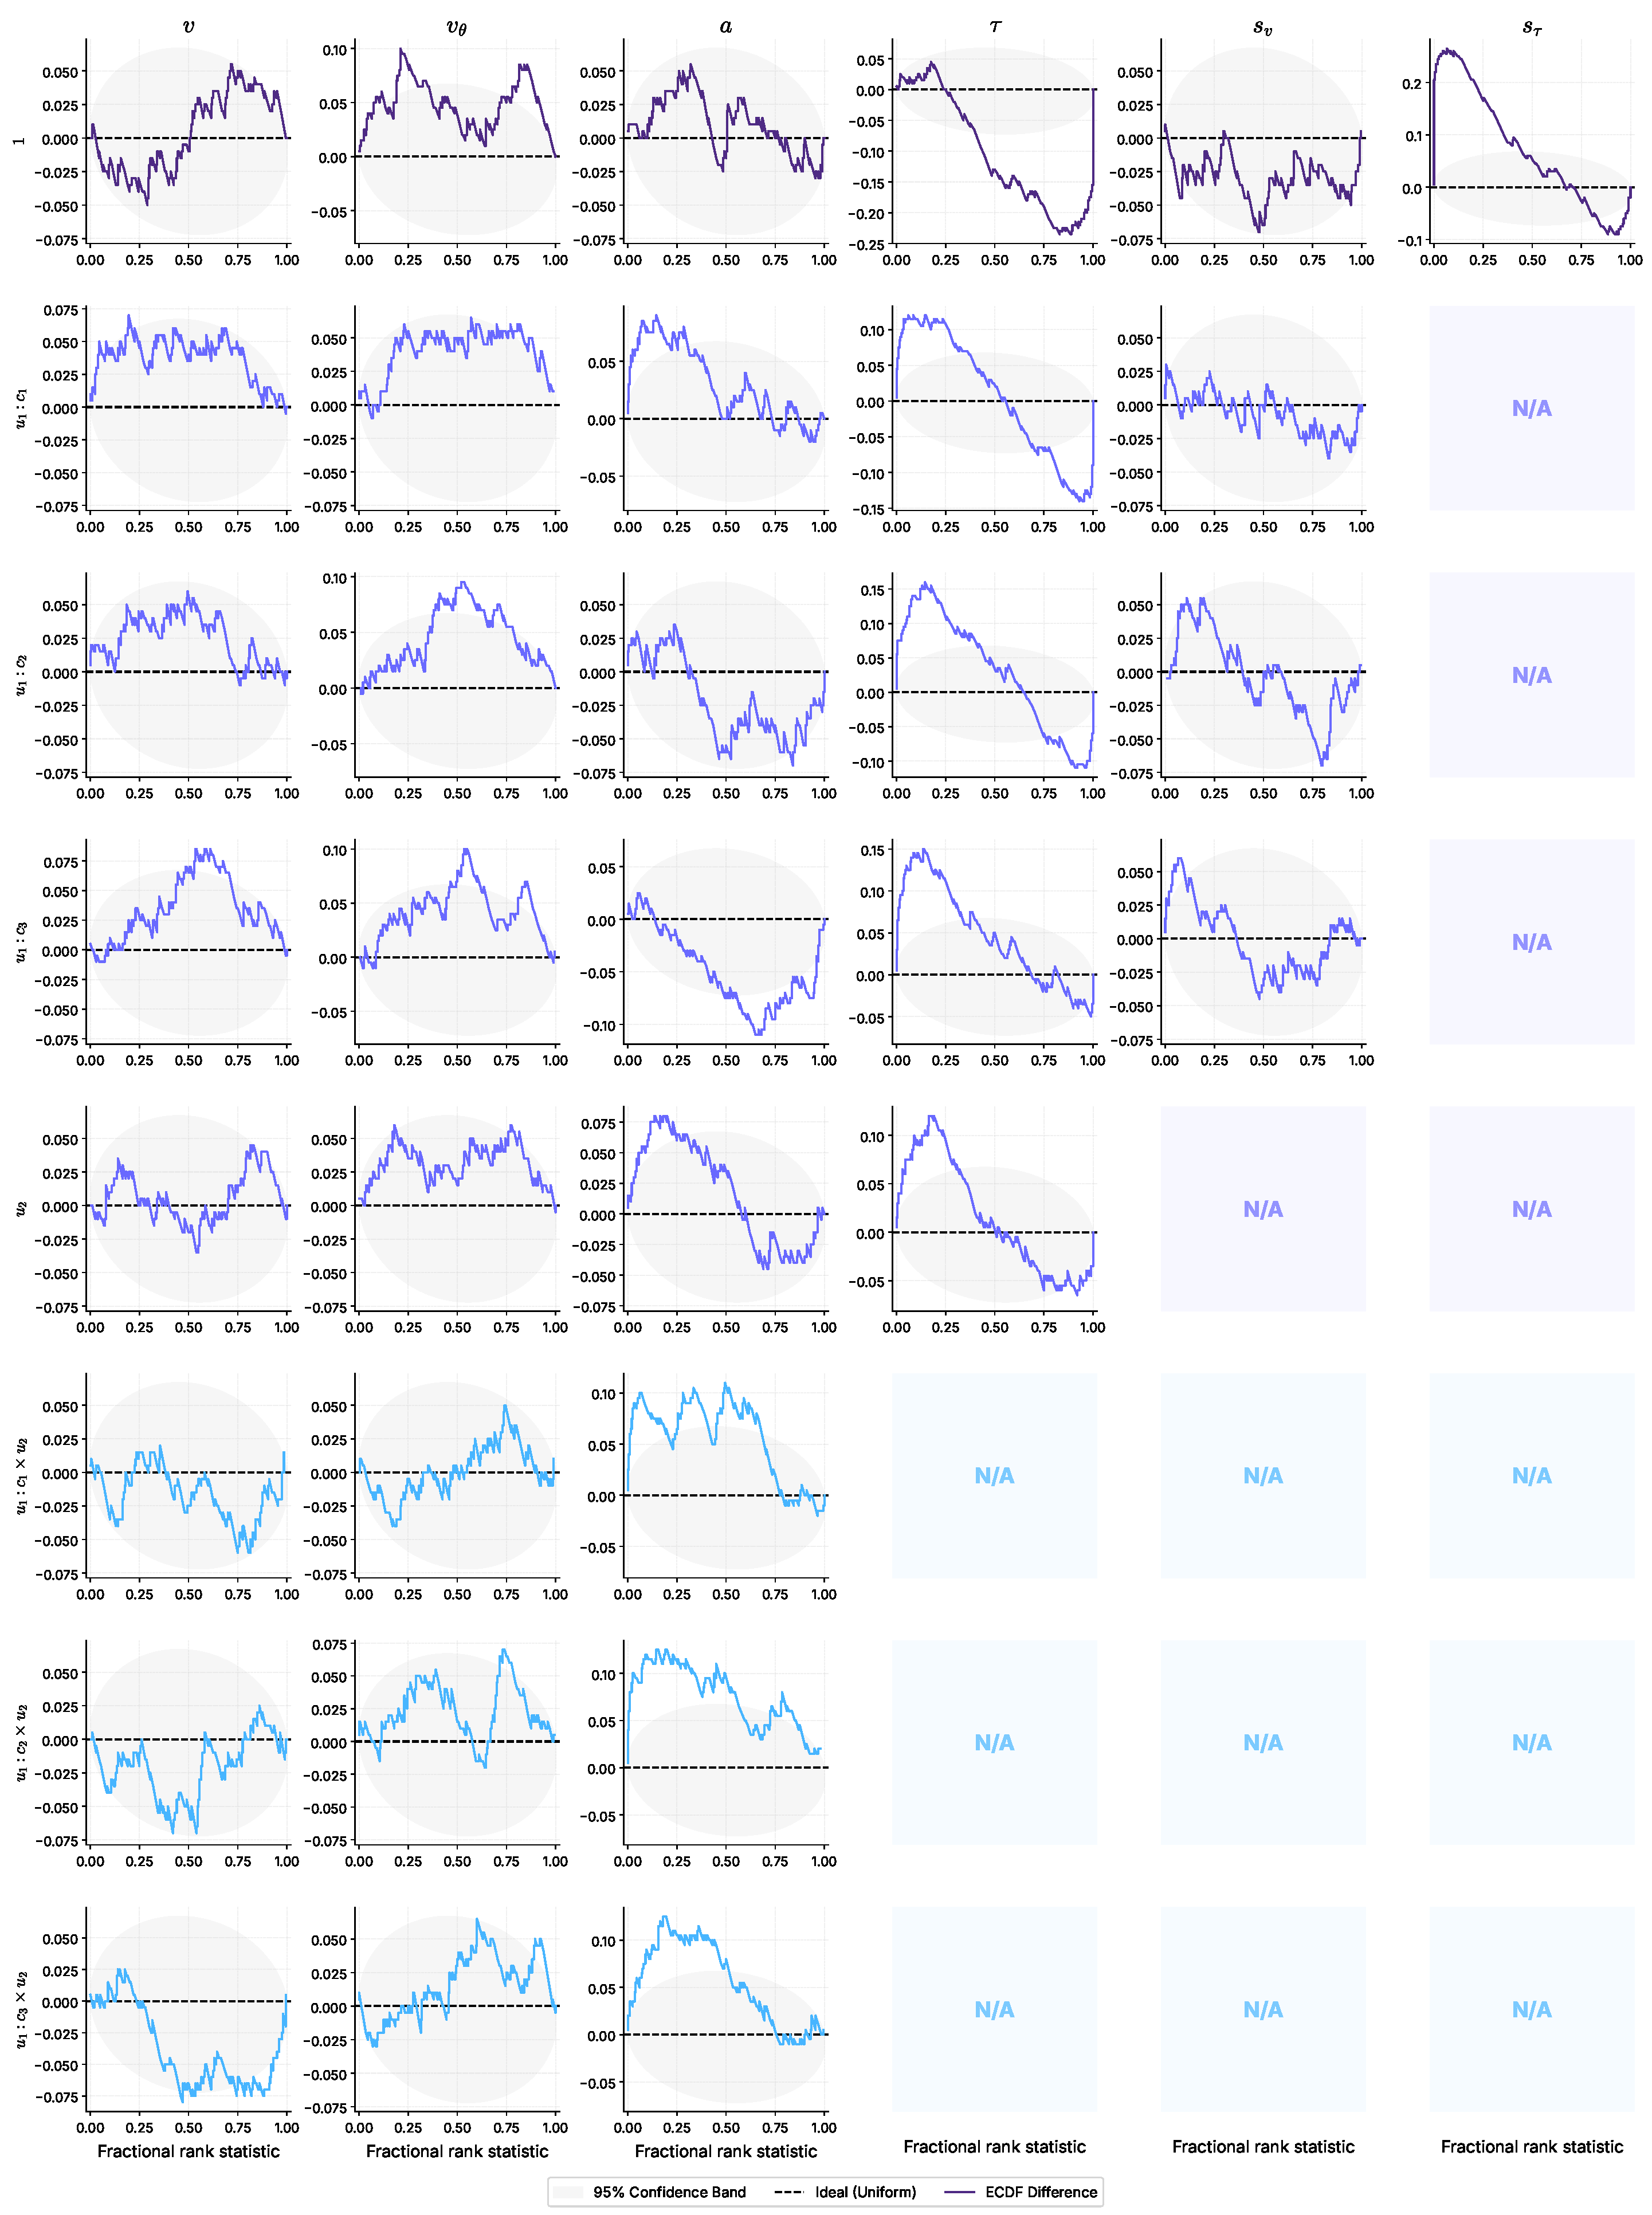
\includegraphics[width=\linewidth,height=0.84\textheight,keepaspectratio]{per_case/cdm/mixed_predictor/ecdf.pdf}
  \caption[CDM, mixed-predictor: ECDF calibration]{\textbf{CDM, mixed-predictor design --- ECDF
    calibration.} Rank-ECDF difference (empirical minus uniform) with simultaneous
    95\% confidence bands, on the same cell layout as the corresponding recovery
    figure (Figure~\ref{fig:e1-cdm-mixed_predictor-rec}). A calibrated posterior stays
    inside the band; excursions above/below indicate bias, and a systematically
    shallow/steep curve indicates over-/under-dispersion.}
  \label{fig:e1-cdm-mixed_predictor-ecdf}
\end{figure}

\FloatBarrier

% --- Restore LaTeX default float parameters -----------------------------------
\renewcommand{\topfraction}{0.7}
\renewcommand{\bottomfraction}{0.3}
\renewcommand{\textfraction}{0.2}
\renewcommand{\floatpagefraction}{0.5}

%=============================================================================
% END OF EXPERIMENT 1 APPENDIX SECTION
%=============================================================================
